\documentclass[letterpaper]{article}

% AAAI-style 2-per-page format, without the annoying bits
\setlength\topmargin{-0.25in} \setlength\oddsidemargin{-0.25in}
\setlength\textheight{9.0in} \setlength\textwidth{7.0in}
\setlength\columnsep{0.375in} \newlength\titlebox \setlength\titlebox{2.25in}
\setlength\headheight{0pt}  \setlength\headsep{0pt}
\flushbottom \sloppy

\pdfpagewidth=8.5in
\pdfpageheight=11in

\usepackage{natbib}

\usepackage{times} 
\usepackage{helvet}  
\usepackage{courier}  
\usepackage{url}  
\usepackage{graphicx} 

\usepackage{amssymb}
\usepackage{amsthm}
\usepackage{amsmath}
\usepackage{algorithm}
\usepackage[noend]{algpseudocode}



\usepackage{multirow}
\usepackage{ctable}
\usepackage{color}
\usepackage{natbib}
\usepackage[normalem]{ulem}


\usepackage{romannum}

%\usepackage[style=authoryear]{biblatex}

\usepackage{hyperref}
\hypersetup{
	colorlinks=true,
	linkcolor=black, % color for table of contents
	citecolor=black, % color for citations
	urlcolor=blue, % color for hyperlinks
	bookmarks=true,
}
\urlstyle{same}




\raggedbottom %nicer enumerate
\theoremstyle{definition}
\newtheorem{defn}{Definition}[section]
\newtheorem{lemma}{Lemma}[section]
\newtheorem{hypothesis}{Hypothesis}[section]
\newtheorem{assumption}{Assumption}
%%%%%%%%%%%%%%%%%%%%%%%%%%%%%%%%%%%%%%%%%%%%%%%%%%%%%%%%%%%%%%%%%%%%%%%%%%%%%%%%%%%%%%%%%%%%%%%%%
\title{Curriculum learning in RL}
\begin{document}
	
	\pagenumbering{arabic}
	\maketitle
	\begin{abstract}
		%Added most methods not focused on varied tasks
		%Added methods focused on task variety and exploration
		%Added short-term goals, blog, POMDP fomulation
		%Added parameter and code base sections, updated goals
		%Added model-based RL section
		%Added experiments section
		%Added ensemble agent ideas
		%Added ML-CL section
		%Wrote formulation of meta PAC-bayes with known task
		
		Fixed probabilistic analysis of error probability
		
		Cleaned up formalization for the multi-task case
		
		Changed limits for convergence if $n/m\rightarrow\infty$
		
		Added explicit statements of assumptions for each subsection
		
		Added a short section on different optimization scheme
		
		Updated short term goals
		
		Added justification to the choice of minimum for expected task loss
		
		Updated the probabilistic formulation with express calculations and a new color
		
		Created a bound for a proportional mix posterior, giving a criterion for the mix parameter
		
		Cleaned up section on task similarities and test data, removing some incorrect statements
		
		Re-phrased the questions for test-task adaptation
		
		Added subsection \ref{subsec:pb-adapt} on domain adaptation and PB
		
		
	\end{abstract}

\tableofcontents
%%%%%%%%%%%%%%%%%%%%%%%%%%%%%%%%%%%%%%%%%%%%%%%%%%%%%%%%%%%%%%%%%%%%%%%%%%%%%%%%%%%%%%%%%%%%%%%%%

%%%%%%%%%%%%%%%%%%%%%%%%%%%%%%%%%%%%%%%%%%%%%%%%%%%%%%%%%%%%%%%%%%%%%%%%%%%%%%%%%%%%%%%%%%%%%%%%%
\section{*Problem formulations - 14.1.21} \label{sec:formulation}
%%%%%%%%%%%%%%%%%%%%%%%%%%%%%%%%%%%%%%%%%%%%%%%%%%%%%%%%%%%%%%%%%%%%%%%%%%%%%%%%%%%%%%%%%%%%%%%%%
\begin{defn}
	A \textbf{task} (sometimes called an environment) is defined as a MDP $<S,A,P,R,\gamma>$,
	Where $S$ is a set of states, $A$ is a set of actions, $P:S\times A\times S\rightarrow [0,1]$ is a transition function, 
	$R:S\times A\rightarrow \mathbb{R}$ is a reward function, $\gamma\in[0,1]$ is a discount factor.
\end{defn}

\begin{defn} \label{defn:curriculum-pomdp}
	Given a (possibly infinite) set of possible tasks $\mathcal{T}$, a \textbf{curriculum} is the policy rollout of the POMDP $<S,A,P,R,\Omega,O, \gamma>$, where:
	\begin{itemize}
		\item $S$ is the (unobserved) set of student states. In the case of neural networks, $s_t$ is the vector of network parameters.
		\item $a_{t}^{\tau, k}\in A$ is the action of training the student on task $\tau\in \mathcal{T}$ for $k$ time steps.
		\item $P$ is the (unobserved) transition function between states. This is determined by the student's learning algorithm.
		\item $R:O\times A\times H \rightarrow \mathbb{R}$ is a reward function that evaluates student performance on a given task, possibly based on observation history $H$.
		\item $o_t$ is the teacher's student observation on the task. This is usually a `black box' observation, meaning $o_t\neq s_t$. Common examples of $o_t$ are the student's task trajectory or the student's discounted return.
	\end{itemize}	
	%\[
	%\max_{D^{\mathcal{T}}} \sum_{T \sim \mathcal{T}_target} {P_T^N dT}
	%\]
\end{defn}

A \textit{teacher algorithm} is defined by specifying the observation method $o_t$ and the teacher's reward $R$. It is often assumed that tasks in $\mathcal{T}$ have the same internal state and action space, with dynamics and task-level rewards varying between tasks.
Note that changing the start state or goal state for a task is also possible, since this is part of the specification of the task.
%There are no works (that I found) that define RL curricula with a control measure smaller than a full episode on a task.

\begin{defn} \label{defn:curriculum-pomdp-shaping}
	A \textbf{reward-shaped curriculum} is a variant curriculum where the actions are different:
	Given a set of tasks $\mathcal{T}=\{\tau|\tau=<\hat{S},\hat{A},\hat{P_i},\hat{R_i},\hat{\gamma}>\}$, the action $a_{t}^{\tau', k}$ is the action of training the student on task $\tau'=<\hat{S},\hat{A},\hat{P_i},R',\gamma'>$ for $k$ time steps, where $\gamma'\leq \hat{\gamma}$ and $R'(s,a)=\hat{R_i(s,a)}+R'(s,a)$ for a given shaped reward $R'$.
\end{defn}

An alternative formulation to the curriculum problem is embedded in game theory:
\begin{defn} \label{defn:curriculum-game-theory}
	A \textbf{collaborative curriculum} is defined according to the following sequential, asymmetric two-player game:
	\begin{itemize}
	\item $H$ is the game's history, and is available to both players.
	\item A teacher player's action is to provide a task $\tau$ and a time step budget $k$,
	\item A student player's action is to train on the given task, as well as other tasks in $H$, for a total time of $k$.
	\item The action-payoff function $v:\mathcal{T}\times \mathbb{N^+} \times H \rightarrow \mathbb{R}\times \mathbb{R}$ is the paired payoff for the teacher and student. 
	\end{itemize}
\end{defn}

We note that this game may be a zero-sum game (the teacher and student have opposed payoffs) or more cooperative, depending on the payoff function.
It is also important to note that if the student is required to perform the given task for all $k$ time steps, and the only goal is to maximize the teacher's payoff, we get a formulation that is equivalent to definition \ref{defn:curriculum-pomdp}, and in fact would be reasonable to solve using reinforcement learning.


%%%%%%%%%%%%%%%%%%%%%%%%%%%%%%%%%%%%%%%%%%%%%%%%%%%%%%%%%%%%%%%%%%%%%%%%%%%%%%%%%%%%%%%%%%%%%%%%%
\section{*Measuring task difficulty and curriculum - 23.2.21} \label{sec:difficulty}
%%%%%%%%%%%%%%%%%%%%%%%%%%%%%%%%%%%%%%%%%%%%%%%%%%%%%%%%%%%%%%%%%%%%%%%%%%%%%%%%%%%%%%%%%%%%%%%%%

In \cite{Matiisen2020}, the task probability is based on the absolute value of the reward improvement rate, measured by the difference between the trained task reward $r_t$ and the trained task reward last measured for the same task $r_{t'}$.
This method only works for a finite set of tasks. Tasks with high improvement or large performance decreases will be sampled more often.

In \cite{Feng2020}, a curriculum is designed for a specific task (Sokoban), and task difficulty is measured by a domain-specific measurement, the number of boxes to be moved to goal locations. Difficulty is increased based on the reverse of \cite{Matiisen2020} - if the success rate on a given difficulty level has not changed for several iterations, difficulty should be increased. This is because measuring task feasibility in Sokoban is hard, and therefore improvement rate can be zero even in cases where the agent does generalize well.

In \cite{Klink2020}, some task parameters are called a `context' (e.g. friction and goal location), and task probability for a given task is based on the student's value function estimate of the start state (including the context).
Contexts are assumed to come from a Gaussian distribution and the target distribution is assumed to be \textbf{known}.
The value function estimate is normalized by the context probability and by KL-divergence from the target distribution to discourage a large gap from the target environment. A KL-divergence constraint is also used to prevent large changes in the context distribution between updates.

In \cite{Jiang2020}, a curriculum is learned in order to re-try previously solved tasks in a manner that would hopefully lead to generalization. Task probability is proportional to the (discounted) TD-error for the last sampled trajectory - this is calculated as $ \frac{1}{T} | \sum_{t=0}^{T} {G_{t:T}}|$, where $G_{t:T}$ is the $t$-step discounted return. Tasks with high TD-error supposedly have higher learning potential, and are therefore more likely to be re-tried. 

In \cite{Portelas2019}, the authors define \textit{ALP-GMM}, a MAB (Multi-Armed Bandit) based teacher, that chooses the environment parameters based on absolute learning progress, the same thing as absolute improvement rate.
Unlike \cite{Matiisen2020}, task parameters are continuous, so they are separated into regions to allow comparisons to previous tasks. The major innovation of \textit{ALP-GMM} is in how to create the separation. A Gaussian Mixture Model is learned to fit task parameters to the improvement rate, giving a better connection between parameter space and improvement rate (compared to random task selection or hard-coded regions which is a method called \textit{RIAC}).
In \cite{Portelas2020}, a continuation of this approach with multiple students was proposed. In this classroom-like setting, the goal is to maximize task selection as well as student selection, meaning schedule must offer both a task and a student to give said task to, and optimizes over all students. \textit{ALP-GMM} is used for task selection, and a knowledge vector for each student is learned and used to select a task that will have good improvement rate for multiple similar students (similarity measured by knowledge vector).

In \cite{Narvekar2019}, a curriculum for grid-world environments is learned with task-specific operators used to specify task simplification (sub-goals and parameter-based simplifications). The curriculum itself measured time to convergence, i.e. the number of episodes until the policy ceases to change. A low time was considered more desirable.
In a continuation paper, \cite{Narvekar2020}, the authors improve on this by measuring convergence with actions instead of episodes, a policy is considered to converge if the number of steps required to reach a goal state is at most $\delta$ more than the optimal policy for a pre-defined $\delta$. The set of tasks is pre-defined, and both a task and a goal must be chosen.

In \cite{Gutierrez2020}, tasks are chosen from a given set based on a combination of relevance and a difference from previously chosen tasks. The relevance criterion is measured using policy entropy. It is assumed that the optimal policy for each task is known, and a set of \textit{validation tasks} similar to the test tasks is given.
A task is considered relevant if for at least one \textit{validation task}, we run the optimal policy in the task, measure mean entropy for the visited states, then train the policy $l$ steps and measure the same entropy, and a lower entropy is reached. Basically, a task is relevant if adapting it to a validation task makes it more deterministic.
Interestingly, they show that choosing all subtasks did not necessarily give better meta-learning.

In \cite{Justesen2018}, a task-specific difficulty measure is defined, and difficulty is increased on task success and decreased on task failure by a fixed amount.

In \cite{Jain2017}, tasks are chosen from a given set, and several selection criteria are defined. Among these criteria are:
\begin{itemize}
	\item Reward maximizing task - run a trajectory on each task, pick task with highest reward.
	\item Transfer maximizing task - before training, estimate task transferability (for example by calculating reward for task b after transferring policy trained on task a) for all task pairs as well as the target task. The curriculum is one that will maximize transferability from some initial task to the target task.
	\item Active reward maximization - assumes each task comes with a feature vector, and use active-learning regression to estimate the transferability between tasks
\end{itemize}
These curriculum were shown to converge more quickly and to a higher reward than learning on the target task directly.

In \cite{Reny2019}, a curriculum for experience re-play is learned. Unlike \cite{Jiang2020}, new tasks are created. This is done by choosing goal states (like HER) that will be difficult but achievable. In the paper, HER is considered a curriculum of choosing goal states estimated to be easy to achieve (via value function estimation), and this paper adds a term to try and pick goals that will have low Wasserstein (earth-mover) distance from the target goal distribution (which is assumed to be known). The choice of Wasserstein distance comes from a theorem assuming that close goals lead to close policies.

In \cite{Dennis2020}, environment parameters are chosen (tasks) to try and create hard but solvable tasks. An adversarial task generator creates a task, the student `protagonist' trains on it, then another `antagonist' agent train on it. The task generator tries to change the environment parameters to maximize `antagonist' return and minimize `protagonist' return (both were trained to convergence on the last environment). This is shown to be a nash-equilibrium between `protagonist' and `antagonist'. The intent is that as student adapts, environment must become more difficult.

In \cite{Racaniere2019}, goal states are chosen (tasks) to try and create hard but solvable tasks. 
This is done by trying to balance a trade-off between three metrics: feasibility, validity, and coverage.
Goal validity (likelihood of student reaching the goal) is measured by the Negative Log-Likelihood of generating a goal that's very close to a previously achieved goal.
Goal feasibility is measured using a binary classifier that tries to predict agent success given a goal. The teacher knows this prediction and uses it when generating environments.
If target goal distribution is known, this is also used to measure the teacher's loss.
The paper evaluated the performance of measures in complex environments, and showed that all metrics were useful.

In \cite{Al-Shedivat2017}, a curriculum is implicitly learned in a multi-player game by adversarial self-play. The paper itself assumes task distribution is given and is similar to existing meta-RL approach MAML (\cite{Finn2017a}).

In \cite{Zhang2020}, a goal state is chosen from a given parameter space. An ensemble of value function estimators (Q was chosen in the paper) is learned, and is used to estimate the standard deviation for given goal and start state. Goals with high standard deviation (=low confidence) are assumed to be good as they should be complex but not impossible.

In \cite{Florensa2017, Florensa2018}, a curriculum based on medium difficulty goal-based tasks is created, using an algorithm called \textit{GoalGAN}. This is done by trying to find a policy to maximize the probability of reaching the goal assuming some known test goal distribution (which was uniform in the paper). Do to so efficiently, goals are sampled from a smaller set of goals (called \textit{GOID}), with estimated success probability between some lower and upper bound. This is done using a GAN, with the discriminator separating goals in \textit{GOID} and goals not in \textit{GOID}, with policy evaluations used as labels (the return should be in the range). Does well compared to self-play and \textit{RIAC}.

A similar approach can be seen in \cite{Srinivasan2019}, where this notion of medium difficulty goals was applied to discrete state and action spaces. In their paper, a curriculum of goals is created by trying to choose start states within certain distance to the goal, but since random walk can be an issue in discrete spaces, demonstrations are used to determine both the start state and the curriculum, as each task is created by following an expert $i$ steps, with $i$ decreasing as the agent improves.

In \cite{Wohlke2020}, a curriculum is learned in order to maximize probability of reaching a known goal state given that the start state is selected uniformly. This is done by changing the distribution of start states to match the $L_2$ norm of the gradient for our performance measurement (probability of reaching the goal). This is estimated by picking a dimension and doing a zeroth-order approximation of the partial derivatives. This only works if the state space is euclidean, but that is quite common. This is quite similar to improvement rate for goal-based rewards.

In \cite{Akkaya2019}, a method to randomize environment parameters was proposed. In each iteration, environment parameters are uniformly sampled from a $d$-dimensional box. To adapt the box size, a random parameter is sampled from one of the edges of its current range, and an episode is trained to measure reward. Once enough data for a parameter is gathered, we measure the average performance and if it is above or below a set threshold, we change the box size. 

In \cite{Fang2020}, a combination of task feasibility and the closeness to the test environment are used to estimate progress. A good curriculum will give tasks closer to the test environment, but still feasible. Task generation is done with a GAN setup: A generator creates tasks (by choosing task parameters), and a discriminator tries to estimate `task progress' - the similarity of the trajectory for the generated task to a trajectory on the test task. To do this, rollouts on the test task are required. The generator loss is a combination of the discriminator error and the task's expected return.

In \cite{Milano2021}, task parameters are chosen from a finite set for use in evaluations of the gradient in an Evolutionary Strategies algorithm. After a warm-up period where tasks are chosen randomly, possible parameters are organized into subsets based on average reward, and evaluations pick randomly from a subset based on this ``difficulty. Notably, they show empirically that dividing subsets into difficulties non-uniformly is preferable, using $x^2$ and $x^3$ as the difficulty measures, thus creating larger subsets of easy tasks and smaller subsets of hard tasks. 

In \cite{Li}, if a goal-conditioned task is not achieved, random search is used to try and find a sub-goal such that the agent can easily reach the original goal from the sub goal. Once data has been collected on the new trajectory to the sub-goal, the agent is updated.

In \cite{Won2019}, a PPO-based agent learns a policy that is robust (to a degree) to changes in body type parameters by giving a curriculum where tasks with low expected rewards are sampled more often. 
The expected reward for a task is estimated from the value function estimates for that task. The resulting trained policy can also adapt to online changes to the body parameters, since the parameters are included in the state representation.

%%%%%%%%%%%%%%%%%%%%%%%%%%%%%%%%%%%%%%%%%%%%%%%%%%%%%%%%%%%%%%%%%%%%%%%%%%%%%%%%%%%%%%%%%%%%%%%%%
\section{*Ensuring task variety - 24.1.21} \label{sec:variety}
%%%%%%%%%%%%%%%%%%%%%%%%%%%%%%%%%%%%%%%%%%%%%%%%%%%%%%%%%%%%%%%%%%%%%%%%%%%%%%%%%%%%%%%%%%%%%%%%%

In \cite{Jiang2020}, a probability bonus is given proportional to the number of tasks seen since a given task was sampled, thus forcing the task to eventually be re-played.

In \cite{Gutierrez2020}, tasks are chosen from a given set based on a combination of relevance and a difference from previously chosen tasks. Difference is measured by the mean KL-divergence of the optimal policies for a pre-defined set of states. A task is different from chosen tasks if the KL-divergence of its optimal policy is sufficiently large.

In \cite{Reny2019}, an optimization constraint for choosing a goal state is imposed, forcing tasks to come from different training trajectories.

In \cite{Racaniere2019}, goal states are chosen (tasks) to try and create hard but solvable tasks. 
This is done by trying to balance a trade-off between three metrics: feasibility, validity, and coverage.
Goal coverage is measured by the entropy of the teacher over random goals.

In \cite{Mehta2019}, environment `difficulty' is estimated by learning a discriminator that tries to separate rollouts from generated environments and rollouts in a given reference environment. The discriminator output is used as the teacher's reward for the generated environment, so environments that are very different from the reference environment are rewarded. 
The teacher agent tries to choose environment parameters to maximize this reward, and therefore encourage variety. The teacher agent uses a method called \textit{SVPG}, Stein Variational Policy Gradient, a method similar to \textit{A2C} but with multiple policy parameters (called particles), and a trade-off between parameter reward and difference between them (measured with a kernel function).
Expanding on the previous apporach, \cite{Raparthy2020} create a method with two teacher agents: one uses a discriminator to force environment parameters away from the reference environment like in \cite{Mehta2019}, and the other that chooses a task from the given distribution in an adversarial manner: the task selector uses the student policy and a stopping policy to act in the reference environment and find a goal state. The student must then reach that goal in the generated environment. To update the stopping policy, the adversary is rewarded for finding a goal in few actions that also requires many actions to reach, and is therefore hopefully hard but solvable. 
In a continuation paper, \cite{Mehta2020}, a meta-RL algorithm is used to adapt the student policy to the generated environment, and the discriminator tries to predict whether the trajectory came from the policy before or after adaptation, thus encouraging tasks with large changes during adaptation. Notably this removes the need to have reference environments.

In \cite{Sukhbaatar2017}, a goal-choosing agent acts in the environment to try and find states that will be difficult to solve. This was the direct inspiration to \cite{Raparthy2020}, and where its stopping policy notion comes from. In a later paper, \cite{OpenAI2021} expanded on this approach by: filtering goal states to goals not solved by the student, the teacher having a set number of time steps to propose goals, and the student measured on achieving one of five generated goals. Additionally, a custom reward function to the teacher, and a clipped behavior cloning loss are used to improve stability.

In \cite{Gupta2018}, the environment parameters are not given directly to the trained student, but are used as latent variables to generate an environment. A discriminator is learned to try and predict the latent task that was used to generate a given trajectory, with high confidence prediction yielding high reward. Since a high variety between tasks leads to good prediction, this helps with variety.

In \cite{Jabri2019}, a curriculum to learn an MDP without a reward is proposed. The teacher agent chooses environment parameters as latent variables, and gives state reward $r_z(s) = log q(s|z) - log q(s)$, the information gain of the latent variable. The teacher agent uses the sampled trajectories to improve this $q$, via discriminative clustering.

In \cite{Kaddour2020}, tasks are characterized by a learned low-dimensional task embedding. This is done by learning an encoder on trajectories that tries to maximize likelihood of parameters and rewards given the observations. To pick a task, a point in the latent space is picked to maximize some utility.
The utility used in the paper was picking maximal surprise (self-information) - a latent point with low likelihood according to the estimate task distribution.

In \cite{Wang2019}, \textit{POET}, a genetic algorithm for varied task generation is proposed. A set of environments and a set of agents are maintained, and at each step, environment parameters are randomly changed (with a ranking based on euclidean distance of parameters from already existing environments), each agent is trained on each environment (using a single step of ES - evolution strategies), and if an environment is challenging (mean reward at least $x$ and at most $y$), it is kept.

%%%%%%%%%%%%%%%%%%%%%%%%%%%%%%%%%%%%%%%%%%%%%%%%%%%%%%%%%%%%%%%%%%%%%%%%%%%%%%%%%%%%%%%%%%%%%%%%%
\section{*Method summary - 1.6.21} \label{sec:summary}
%%%%%%%%%%%%%%%%%%%%%%%%%%%%%%%%%%%%%%%%%%%%%%%%%%%%%%%%%%%%%%%%%%%%%%%%%%%%%%%%%%%%%%%%%%%%%%%%%

See table \ref{methods-table}

\begin{table*}
%\centering
\caption{Comparison of approaches}
\label{methods-table}
\begin{tabular}{|l | l | l | l  | l|l|} 
	\hline
	Paper & good paper & Difficulty measure & variety measure  & Controllable elements     \\ \hline	
	\cite{Matiisen2020}& seminal & improvement rate & none & task selection  \\ \hline
	\cite{Feng2020}& & domain-specific & none & task parameters  \\ \hline
	\textit{SPRL} \cite{Klink2020}& multi-env & $V(s_0)$ & none & task parameters \\ \hline
	\cite{Jiang2020} & multi-env & improvement potential (error) & uncertainty bonus & task selection  \\ \hline
	\textit{ALP-GMM} \cite{Portelas2019} & &  improvement rate & none & task parameters \\ \hline
	\cite{Portelas2020} & & improvement rate & none & task parameters, student  \\ \hline
	\cite{Narvekar2019} & & fast policy convergence & none & task parameters \\ \hline
	\cite{Narvekar2020} & curriculum works & fast policy convergence & none & task selection, goal state \\ \hline
	\cite{Gutierrez2020} & good theory & validation tasks & Policy KL-divergence & task selection \\ \hline
	\cite{Justesen2018} & & $\pm$ difficulty, on success/fail & none & task parameter \\ \hline
	\cite{Jain2017} & & transfer improvement & none & task selection \\ \hline
	\cite{Reny2019} & & $V(s_0)-diff(g,g*)$ & Constrained goals & start state, goal state \\ \hline
	\textit{PAIRED} \cite{Dennis2020} & Unsupervised SoTA & adversarial reward & none & task parameters \\ \hline
	\cite{Racaniere2019} & multi-env, deepmind & prob of task success & teacher entropy & goal state \\ \hline
	\cite{Al-Shedivat2017} & & self-play & none & opponent agent \\ \hline
	\cite{Zhang2020} & multi-env & ensemble confidence & none & goal state \\ \hline
	\cite{Wohlke2020} & & $\sim V'(s_0)$ & none & start state \\ \hline
	\cite{Fang2020} & multi-env, ok theory & improvement rate \& test diff & none (GAN helps) & task parameters \\ \hline
	\textit{GoalGAN} \cite{Florensa2018} & seminal & return in range & none (GAN helps) & goal state \\ \hline
	\cite{Mehta2019} &  & none & learned trajectory difference & task parameters \\ \hline
	\cite{Raparthy2020} & & adversarial reward & learned trajectory difference & task parameters \\ \hline
	\cite{Sukhbaatar2017} & multi-env, ok theory & adversarial reward & None & task parameters \\ \hline
	\cite{OpenAI2021} & openAI, multi-env & adversarial reward & new goals & task parameters \\ \hline
	\cite{Mehta2020} & multi-env, metaRL & none & learned adaptation difference & task parameters \\ \hline
	\cite{Gupta2018} & & none & learned state difference & task parameters \\ \hline
	\cite{Jabri2019} & & none & trajectory clustering & task parameters \\ \hline
	\cite{Srinivasan2019} & & demonstrated trajectories & none & start state \\ \hline
	\cite{Akkaya2019} & & return, fixed change size & none & task parameters \\ \hline
	\cite{Kaddour2020} & multi-env, ok theory & none & surprise (low likelihood) & task parameters \\ \hline
	\textit{POET} \cite{Wang2019} & & return in range & distance in parameter space & task parameters \\ \hline
	\cite{Milano2021} & & average reward & none & task parameters \\ \hline
	\cite{Li} & & solved before & none & sub-goal \\ \hline
	\cite{Won2019} & & expected $V(s|p)$ & none (sampling) & task parameters \\ \hline
	
\end{tabular}
\end{table*}

%%%%%%%%%%%%%%%%%%%%%%%%%%%%%%%%%%%%%%%%%%%%%%%%%%%%%%%%%%%%%%%%%%%%%%%%%%%%%%%%%%%%%%%%%%%%%%%%%
\section{*Curriculum learning in ML - 18.6.21} \label{sec:CLML}
%%%%%%%%%%%%%%%%%%%%%%%%%%%%%%%%%%%%%%%%%%%%%%%%%%%%%%%%%%%%%%%%%%%%%%%%%%%%%%%%%%%%%%%%%%%%%%%%%

To begin, let us discuss ``self-paced learning'' (SPL), a common form of easy-to-hard curriculum.
SPL refers to curricula where each example is weighted based on the model error in a specific manner.
In SPL, an EM algorithm is used to jointly optimize example weights $v_i$ and model parameters $w$.

$w$ is optimized by minimizing weighted loss for any loss function $l$.
$v$ is optimized by minimizing $v^*(l,\lambda)=argmin_{v} vl + f(v, \lambda)$, where $\lambda$ is a monotonically increasing ``age'' parameter, and $f$ is the self-paced regularizer function, that must satisfy:
\begin{enumerate}
	\item $f(v, \lambda)$ is convex with respect to $v, l$
	\item $v^*(l,\lambda)$ monotonically decreases as l increases with limits at 0 and infinity (easy samples have more weight)
	\item $v^*(l,\lambda)$ monotonically increases as $\lambda$ increases with limits at 0 and infinity (as training progresses, more examples should be included)
\end{enumerate}

% Optimization math
In \cite{Meng2017}, a connection between SPL and majorization minimization (MM) methods is established, and using existing theory for MM methods, \emph{they derive a proof of convergence}. They also use this theory and connections between the self-paced regularizer and non-convex regularized penalties to show that SPL methods work well in problems with outliers or noisy examples, since the SPL regularizer limits the effect of examples with high loss on the early training. This happens since the conditions mean that high-loss examples have constant loss, and thus gradient methods have zero gradient on these examples and they do not impact training.

In a later paper, \cite{Liu2018}, a connection between SPL and concave conjugates is shown ($v$ is the concave conjugate for $f$).
This fact is used to reduce the condition set on the regularizer to:
\begin{enumerate}
	\item $f(v, \lambda)$ is strictly convex with respect to $v$
	\item $f(v, \lambda)$ is lower semi-continuous with respect to $v$
	\item $f$ covers all of $[0,1]$
\end{enumerate}
These simplified conditions help designing regularizers, as any regularizer satisfying these for constant $\lambda$ can be used as $f(v, \lambda)=\lambda f(v)$. This simpler condition can be used for curriculum design such as partial order, grouping of examples with similar losses and more.

%PAC-BAYES
In a series of papers, \citet{Pentina2015} show that the similarity between tasks may be an important factor to overall performance. In both a lifelong learning setting (like curriculum learning, but the input tasks are chosen randomly, and the goal is few-shot learning on new tasks) and multi-task learning (like lifelong learning, but with a single learner), the empirical risk can be bounded by a combination of the empirical training error and a factor of task dependence - either the size of the dependency set or the mean difference between tasks (this assumes task weights correspond to task similarity, unlikely to happen for complex models or complex task dependencies)

%PAC-BAYES
Two very recent papers extend these results to meta-learning, \cite{Ding2021} and \cite{Cioba2021}.
In the first one, they relax the assumption that the number of examples in the target tasks is similar to the number of examples in training tasks, leading to a bound that corresponds to the (small) number of examples in the target task, but introduces an error term related to the gap between training and target tasks. Using a subsampling method a tighter bound on the risk can be achieved (this means fewer examples are used for training, all examples are used for risk estimation).

In the second paper, they discuss whether it is better to have many tasks with few labels or few tasks with many labels. They show that for MAML with mixed linear regression, there is an optimal trade-off between number of tasks and labels per task for uniform tasks. They also show empirical experiments suggesting that a hard task requires more data, and that it is preferable to assign slightly more data to easy tasks.

% optimization math with some PAC-bayes
Another area of research that recently made use of curricula is semi-supervised learning, where \cite{Gong2019} show that a easy-to-hard curriculum can help with label propagation. 
It is assumed that every example contains $v$ modalities (feature groups) that correspond to $v$ subgraphs of related data points.
A difficulty metric based on distances is constructed, and they prove that an algorithm with a committee of teachers based on each modality to decide how to propagate labels converges in linear time.
They also prove that choosing by the weighted voting has bounded error risk (vs random choice) proportional to the difficulty threshold - if only easy examples are allowed, the error risk is low, but performance is worse since fewer examples are considered. This means that weighted voting is good.

% geometry
In \cite{Weinshall2018, Weinshall2020}, the authors define two notations: the global difficulty of an example is the loss for that example given an optimal hypothesis, and the local difficulty of an example is the loss given the current hypothesis.
For a linear hypothesis class under a convex loss, they prove that a curriculum ranked by low global difficulty leads to faster convergence. They also prove that, given identical global difficulty, \emph{high} local difficulty is preferable. They show this empirically by using a pre-trained network as an estimator of global difficulty.
This result is empirically reinforced by a later paper (\cite{Hacohen2019}), showing that the easy-to-hard curriculum improves transfer accuracy, and a hard-to-easy curriculum harms transfer accuracy.


%%%%%%%%%%%%%%%%%%%%%%%%%%%%%%%%%%%%%%%%%%%%%%%%%%%%%%%%%%%%%%%%%%%%%%%%%%%%%%%%%%%%%%%%%%%%%%%%%
%\section{The Meta-Curriculum problem - 24.6.21} \label{sec:mcl}
%%%%%%%%%%%%%%%%%%%%%%%%%%%%%%%%%%%%%%%%%%%%%%%%%%%%%%%%%%%%%%%%%%%%%%%%%%%%%%%%%%%%%%%%%%%%%%%%%

%\begin{defn} \label{defn:mcl}
%	A \textbf{meta-curriculum problem} is characterized by:
%	\begin{itemize}
%		\item A task probability distribution $\mathcal{T}$, $(\mathcal{D}_i, m_i)\sim \mathcal{T}$. We will mark $S_{i}=\{(x_j, y_j)\sim \mathcal{D}_i\}_{j=1}^{m_i}$
%		\item A Hypothesis class $H$
%		\item A loss measure $\mathcal{L}: S\times H \rightarrow \mathbb{R}$
%		\item A training set $S=\{S_1,...,S_n\}$
%	\end{itemize}
%
%	Given these, we would like to find a hyper-prior $\mathcal{P}_S$ and learn a hyper-posterior $\mathcal{Q}$ to minimize the multi-task error $\mathcal{L}(\mathcal{Q}, \mathcal{T}) \triangleq \mathbb{E}_{P\sim \mathcal{Q}} \mathbb{E}_{(\mathcal{D}, m)\sim \mathcal{T}} \mathbb{E}_{S\sim \mathcal{D}} [\mathcal{L}(Q(S, P), \mathcal{D})]$ \footnote{$Q$ is a base learner mapping data and prior over $H$ to posterior over $H$}. 
%	To approximate this, we use the empirical multi-task error $\mathcal{\hat{L}}(\mathcal{Q}, S_1,...,S_n) \triangleq \mathbb{E}_{P\sim \mathcal{Q}} [\frac{1}{n} \sum_{i=1}^{n} \mathcal{\hat{L}}(Q(S_i, P), S_i)]$
%\end{defn}


%%%%%%%%%%%%%%%%%%%%%%%%%%%%%%%%%%%%%%%%%%%%%%%%%%%%%%%%%%%%%%%%%%%%%%%%%%%%%%%%%%%%%%%%%%%%%%%%%
\section{*Notable empirical results in CL - 24.6.21} \label{sec:empirical-cl}
%%%%%%%%%%%%%%%%%%%%%%%%%%%%%%%%%%%%%%%%%%%%%%%%%%%%%%%%%%%%%%%%%%%%%%%%%%%%%%%%%%%%%%%%%%%%%%%%%

In \cite{Anonymous2021}, the effect of several difficulty-based curricula is checked.
Task difficulty is checked by one of three methods:
\begin{enumerate}
	\item A reference loss (pre-trained model)
	\item A novel measure called learned iteration, the first iteration where the model output was correct
	\item The c-score, an approximation of generalization accuracy for an example, measured by the expected accuracy for a model trained on n random examples (that are not the measured example)
\end{enumerate}
Additionally, several pacing functions for the size of training sets were examined.
For large datasets with long training times, curricula had no effect, and pacing was marginally useful to improve convergence rate. For short training times or datasets with noisy labels, curricula showed a significant improvement in performance, especially easy-to-hard curricula.

In \cite{Hacohen2019}, A similar experiment is performed with a reference loss function. Results here show a significant improvement for short training times


%%%%%%%%%%%%%%%%%%%%%%%%%%%%%%%%%%%%%%%%%%%%%%%%%%%%%%%%%%%%%%%%%%%%%%%%%%%%%%%%%%%%%%%%%%%%%%%%%
\section{*Notable empirical results in Meta-ML - 24.6.21} \label{sec:empirical-meta}
%%%%%%%%%%%%%%%%%%%%%%%%%%%%%%%%%%%%%%%%%%%%%%%%%%%%%%%%%%%%%%%%%%%%%%%%%%%%%%%%%%%%%%%%%%%%%%%%%

For meta learning, a good reference point is MAML (\cite{Finn2017})), showing a major improvement over previous methods for few-shot transfer.
These results were incrementally improved by REPTILE (\cite{Nichol2018}), by using a Polyak update for the model parameters instead of directly applying the gradient.

Recent approaches (\cite{Saglietti2021, Khodak2019}) that use the data or other expert knowledge to estimate task hardness for meta-learning yield slightly better results for zero-shot and one-shot transfer, with comparable few-shot transfer. 
Both methods do not show a significant improvement over existing methods.
Mentor-Net (\cite{Jiang2017}) is another paper that suggests learning the difficulty of tasks and using it for a curriculum. This method does improve on existing approaches, but this may be due to having a larger network.
Interestingly, Mentor-Net shows a significant improvement over a non-curriculum based approach with similar network sizes, for a setting with noisy labels. This suggests that results from traditional CL literature also hold for the meta-learning case.

Some very recent papers (\cite{Bateni2020, Tian2020}) show that a good representation is more meaningful for effective meta learning, yielding results that are far better than MAML and REPTILE, mostly by using a deeper network and some minor tweaks such as a different loss aggregation or network distillation. 
These methods suggest that the current bottleneck for better meta learning is the representation, and that curricula that impose an effective order on complex representations may be highly useful.

%%%%%%%%%%%%%%%%%%%%%%%%%%%%%%%%%%%%%%%%%%%%%%%%%%%%%%%%%%%%%%%%%%%%%%%%%%%%%%%%%%%%%%%%%%%%%%%%%
\section{*Math for PAC-Bayesian meta learning - 24.8.21} \label{sec:bayes}
%%%%%%%%%%%%%%%%%%%%%%%%%%%%%%%%%%%%%%%%%%%%%%%%%%%%%%%%%%%%%%%%%%%%%%%%%%%%%%%%%%%%%%%%%%%%%%%%%

\subsection{*Definitions and previous results} 

Let $\mathcal{T}$ be an unknown task distribution, let $\mathcal{P}$ be a \emph{hyper-prior} over distributions of hypotheses (data-free). Let $\tau_i=(\mathcal{D}_i, S_i)~\mathcal{T}$ be a set of tasks ($i=1,...,n$).

We assume for now that $\tau_i$ are drawn i.i.d. from $\mathcal{T}$.

We wish to bound the learned \emph{hyper-posterior} $\mathcal{Q}$, and its error - 
$$\mathcal{L}(\mathcal{Q}, \mathcal{T})=\mathbb{E}_{P\sim \mathcal{Q}}[\mathbb{E}_{(\mathcal{D}, m)\sim \mathcal{T}}[\mathbb{E}_{S\sim \mathcal{D}^m}[\mathcal{L}(Q(S,P), D)]]]$$

Using the result from \cite{Rothfuss2020}, by applying the change of measure inequality (see lemma 4 in \cite{Seldin2010}), for any $\lambda>0$,
$$\mathcal{L}(\mathcal{Q}, \mathcal{T})\leq \mathcal{L}(\mathcal{Q}, \mathcal{D}_1,...,\mathcal{D}_n) + \frac{1}{\lambda} KL(\mathcal{Q}||\mathcal{P})+\Upsilon^{\text{\Romannum{2}}}(\lambda)$$

Where $\Upsilon^{\text{\Romannum{2}}}(\lambda)=\frac{1}{\lambda}ln \mathbb{E}_{P\sim \mathcal{P}} [e^{\frac{\lambda}{n}\sum_{i=1}^{n}\mathbb{E}_{(D,S)\sim \mathcal{T}}[\mathcal{L}(Q(P,S),D)- \mathcal{L}(Q(P, S_i), \mathcal{D}_i)]}]$

%\subsection{Math for appendix}

%We note that for any $P\sim \mathcal{Q}$, $P$ is a data-dependent prior (and $P\sim \mathcal{P}$ is a data-free prior).
%From Rivasplata et al (TODO: cite), we know that for each task $i$, given a data-dependent prior $P$,
%$$\Pr_{S_i\sim D_i}\Bigl ( \mathcal{L}(\mathcal{Q}, D_i)\leq \mathcal{L}(\mathcal{Q}, S_i) + KL(Q(P,S_i)||P) + ln(\frac{\xi_i(P)}{\delta_i}) \Bigr )\geq 1-\delta_i$$

%We will mark $Q_i:=Q(P,S_i)$ for comfort.
%By using a union bound (with a known identity connecting union and intersection), and by choosing $\delta_i=\frac{\delta}{n}$ for some $\delta>0$, we get:

%With probability at least $1-\delta$ over the choice of training data $S1,..,S_n$,
%$$\mathbb{E}_{P\sim \mathcal{Q}} \bigl [ \frac{1}{n}\sum_i \mathcal{L}(\mathcal{Q}, D_i) \Bigr ] \leq \mathbb{E}_{P\sim \mathcal{Q}} \bigl [ \frac{1}{n}\sum_i \hat{\mathcal{L}}(\mathcal{Q}, S_i) + \frac{1}{n}\sum_i KL(Q_i||P) + \frac{1}{n}\sum_i ln(\frac{\xi_i(P)}{\delta/n}) \Bigr ]$$


%By definition of $ \mathcal{L}(\mathcal{Q}, \mathcal{D}_1,...,\mathcal{D}_n)$,  $ \hat{\mathcal{L}}(\mathcal{Q}, S_1,...,S_n)$ we get:

%$$\mathcal{L}(\mathcal{Q}, \mathcal{D}_1,...,\mathcal{D}_n) \leq \hat{\mathcal{L}}(\mathcal{Q}, S_1,...,S_n) + \frac{1}{n}\sum_i \mathbb{E}_{P\sim \mathcal{Q}} \bigl [KL(Q_i||P) \Bigr ] + \mathbb{E}_{P\sim \mathcal{Q}} \bigl [ \frac{1}{n}\sum_i ln(\frac{\xi_i(P)}{\delta/n}) \Bigr ]$$

%Developing this further,

%$$ \mathbb{E}_{P\sim \mathcal{Q}} \bigl [ \frac{1}{n}\sum_i ln(\frac{\xi_i(P)}{\delta/n}) \Bigr ] = \mathbb{E}_{P\sim \mathcal{Q}} \bigl [ \frac{1}{n}ln(\frac{\Pi_i\xi_i(P)}{(\delta/n)^n}) \Bigr ] = \mathbb{E}_{P\sim \mathcal{Q}} \bigl [ ln(\frac{(\Pi_i\xi_i(P))^{\frac{1}{n}}}{(\delta/n)}) \Bigr ]$$

%We note that by the definition of $xi_i$,

%$$\mathbb{E}_{P\sim \mathcal{Q}} \bigl [ ln(\frac{(\Pi_i\xi_i(P))^{\frac{1}{n}}}{(\delta/n)}) \Bigr ] = 
%\mathbb{E}_{P\sim \mathcal{Q}} \mathbb{E}_{h\sim P} \bigl [ ln(\frac{(\Pi_i e^{\mathcal{L}(h, \mathcal{D}_i)- \hat{\mathcal{L}}(h, S_i)})^{\frac{1}{n}}}{(\delta/n)}) \Bigr ] = 
%\mathbb{E}_{P\sim \mathcal{Q}} \mathbb{E}_{h\sim P} \bigl [ ln(\frac{ e^{\frac{1}{n}\sum_i\mathcal{L}(h, \mathcal{D}_i)- \hat{\mathcal{L}}(h, S_i)}}{(\delta/n)}) \Bigr ]$$

%Using Jensen's inequality,

%$$\mathbb{E}_{P\sim \mathcal{Q}} \mathbb{E}_{h\sim P} \bigl [ ln(\frac{ e^{\frac{1}{n}\sum_i\mathcal{L}(h, \mathcal{D}_i)- \hat{\mathcal{L}}(h, S_i)}}{(\delta/n)}) \Bigr ] \leq ln \mathbb{E}_{P\sim \mathcal{Q}} \mathbb{E}_{h\sim P} \bigl [ \frac{ e^{\frac{1}{n}\sum_i\mathcal{L}(h, \mathcal{D}_i)- \hat{\mathcal{L}}(h, S_i)}}{(\delta/n)} \Bigr ] = ln(\frac{n}{\delta})+ ln \mathbb{E}_{P\sim \mathcal{Q}} \mathbb{E}_{h\sim P} \bigl [ e^{\frac{1}{n}\sum_i\mathcal{L}(h, \mathcal{D}_i)- \hat{\mathcal{L}}(h, S_i)} \Bigr ]$$

%\subsection{Summary}

%Putting it all together, for any $\lambda>0$ with probability at least $1-\delta$,

%$$\mathcal{L}(\mathcal{Q}, \mathcal{T}) \leq \hat{\mathcal{L}}(\mathcal{Q}, S_1,...,S_n) + \frac{1}{\lambda} KL(\mathcal{Q}||\mathcal{P}) + \frac{1}{n}\sum_i \mathbb{E}_{P\sim \mathcal{Q}} \bigl [KL(Q_i||P) \Bigr ] + ln(\frac{n}{\delta})+ ln \mathbb{E}_{P\sim \mathcal{Q}} \mathbb{E}_{h\sim P} \bigl [ e^{\frac{1}{n}\sum_i\mathcal{L}(h, \mathcal{D}_i)- \hat{\mathcal{L}}(h, S_i)} \Bigr ] +\Upsilon^{\text{\Romannum{2}}}(\lambda)$$

%Using the same method on the change of measure, we can also get:

%$$\mathcal{L}(\mathcal{Q}, \mathcal{T}) \leq \hat{\mathcal{L}}(\mathcal{Q}, S_1,...,S_n) + \frac{1}{\lambda} KL(\mathcal{Q}||\mathcal{P}) + \frac{1}{n\beta}\sum_i \mathbb{E}_{P\sim \mathcal{Q}} \bigl [KL(Q_i||P) \Bigr ] + ln(\frac{n}{\delta})+ \frac{1}{\beta}ln \mathbb{E}_{P\sim \mathcal{Q}} \mathbb{E}_{h\sim P} \bigl [ e^{\frac{\beta}{n}\sum_i\mathcal{L}(h, \mathcal{D}_i)- \hat{\mathcal{L}}(h, S_i)} \Bigr ] +\Upsilon^{\text{\Romannum{2}}}(\lambda)$$

%Whereas the bound in Rothfuss is (for any $\lambda,\beta>0$):

%$$\mathcal{L}(\mathcal{Q}, \mathcal{T}) \leq \hat{\mathcal{L}}(\mathcal{Q}, S_1,...,S_n) + (\frac{1}{\lambda}+\frac{1}{n\beta}) KL(\mathcal{Q}||\mathcal{P}) + \frac{1}{n\beta}\sum_i \mathbb{E}_{P\sim \mathcal{Q}} \bigl [KL(Q_i||P) \Bigr ] + \frac{1}{\beta}ln\mathbb{E}_{P\sim \mathcal{P}}\mathbb{E}_{h\sim P}\bigl [ e^{\frac{\beta}{n}\sum_i\mathcal{L}(h,\mathcal{D}_i)- \hat{\mathcal{L}}(h, S_i)} \bigr ] +\Upsilon^{\text{\Romannum{2}}}(\lambda)$$

%We also note that the term $ln(\frac{n}{\delta})$ is the result of a union bound, and it is possible to replace it with $\sum_i ln(\frac{1}{\delta_i})$. This union bound may be overly pessimistic as it assumes that the \emph{hyper-posterior} is independently bounded for each task. If tasks are not independent it may be possible to use that to derive a tighter bound. We also note that the per-task moment term is now with respect to $\mathcal{Q}$ and not $\mathcal{P}$. 

%\subsection{Analysis}

%If we assume that the per-task moment is not worse in expectation under $\mathcal{Q}$ compared to $\mathcal{P}$, we get: 

%$$\mathcal{L}(\mathcal{Q}, \mathcal{T}) \leq \hat{\mathcal{L}}(\mathcal{Q}, S_1,...,S_n) + \frac{1}{\lambda} KL(\mathcal{Q}||\mathcal{P}) + \frac{1}{n\beta}\sum_i \mathbb{E}_{P\sim \mathcal{Q}} \bigl [KL(Q_i||P) \Bigr ] + ln(\frac{n}{\delta})+ 1+\frac{1}{\beta}ln K +\Upsilon^{\text{\Romannum{2}}}(\lambda)$$

%compared to 

%$$\mathcal{L}(\mathcal{Q}, \mathcal{T}) \leq \hat{\mathcal{L}}(\mathcal{Q}, S_1,...,S_n) + (\frac{1}{\lambda}+\frac{1}{n\beta}) KL(\mathcal{Q}||\mathcal{P}) + \frac{1}{n\beta}\sum_i \mathbb{E}_{P\sim \mathcal{Q}} \bigl [KL(Q_i||P) \Bigr ] + 1+\frac{1}{\beta}ln(K) +\Upsilon^{\text{\Romannum{2}}}(\lambda)$$

%(Since $\frac{1}{\beta}ln(e^{\beta}K)=1+\frac{1}{\beta}ln(K)$)

%Comparing the two bounds is difficult, since the latter depends on $\beta$, commonly a function of $m$ (the size of each task), but our new bound seems inferior.

%\subsection{Gibbs analysis}

%Let us assume that $P\sim \mathcal{Q}$ behaves as follows:
%$$P_{S_i}(h)\propto e^{-\gamma \hat{L}(h,S_i)}P_0(h)$$
%Where $P_0\sim \mathcal{P}$. One method to achieve this is to learn a prior per task, and given a task to use the appropriate prior (this assumes the task is known). This is a naive algorithm that essentially ignores the meta-learning setting, but still gives us an interesting bound:

%From Rivasplata (cite), for each specific task, with probability at least $1-\delta_i$,
%$$L(P,D_i)-L(P,S_i)\leq \frac{1}{\sqrt{m_i}}\bigl ( KL(Q_i||P) + 2(1+\frac{2\gamma}{\sqrt{m_i}})+ln(\frac{1+\sqrt{e}}{\delta_i}) \bigr )$$

%Using a union bound, with probability at least $1-\delta$,
%$$L(P,\{D_i\})-L(P,\{S_i\})\leq \frac{1}{\sqrt{m}}\bigl ( \sum_i KL(Q_i||P) + 2(1+\frac{2\gamma}{\sqrt{m}})+ln(\frac{m(1+\sqrt{e})}{\delta}) \bigr )$$

%Combining with Rothfuss, with $\lambda=n$ we get:

%$$L(P,\mathcal{T})-L(P,\{S_i\})\leq \frac{1}{n}KL(\mathcal{Q}||\mathcal{P}) + \frac{1}{\sqrt{m}}\sum_i KL(Q_i||P) + 2(\frac{1}{\sqrt{m}}+\frac{2\gamma}{m})+\frac{1}{\sqrt{m}}ln(\frac{m(1+\sqrt{e})}{\delta}) + \Upsilon^{\text{\Romannum{2}}}(n)$$
	
%We note that under mild assumptions on the learner $Q$, we get that as $m\rightarrow\infty$, all terms dependent on $m$ go to zero, and as $n\rightarrow\infty$, all terms dependant on $n$ go to zero.

\subsection{*Task dependencies - 29.8.21} \label{sec:bayes:dependencies}

Suppose we know something more about tasks. Can we devise a better bound?
As an initial case, let's start with an easy case.

Let us assume that the goal task is known and was seen during training, that is, we know that we wish to bound $\mathcal{L}(\mathcal{Q}, D_i)=E_{P\sim \mathcal{Q}}E_{S\sim D_i^{m_i}}\mathcal{L}(Q(P, S), D_i)$, where we already have another dataset $S_i\sim D_i^{m_i}$. We will mark $\{D_k\}:=\{D_1,...,D_n\}, \{S_k\}:=\{S_1,...,S_n\}$ for ease of notations.

\subsubsection*{Approach 1 - 4.8.21}
Let us try to bound
$$E_{P\sim \mathcal{Q}}\bigl [E_{S\sim D_i^{m_i}}\mathcal{L}(Q(P, S), D_i)-\hat{\mathcal{L}}(Q(P, S_i), S_i)\bigr ]$$

Using the change of measure inequality, we get (for any $\gamma$)

\begin{equation} \label{eq-base}
\begin{split}
E_{P\sim \mathcal{Q}}E_{S\sim D_i^{m_i}}\mathcal{L}(Q(P, S), D_i)\leq E_{P\sim \mathcal{Q}}\hat{\mathcal{L}}(Q_i, S_i)  + \frac{1}{\gamma}KL(\mathcal{Q}||\mathcal{P})+ \frac{1}{\gamma}E_{P\sim \mathcal{Q}}KL(Q_i||P)\\  +lnE_{P\sim \mathcal{P}}E_{h\sim P}\left [e^{\gamma E_{S\sim D_i^{m_i}}\mathcal{L}(h, D_i)-\hat{\mathcal{L}}(h, S_i)}\right ]
\end{split}
\end{equation}

To minimize this, we would like to balance minimizing $E_{P\sim \mathcal{Q}}\hat{\mathcal{L}}(Q_i, S_i)$ and $KL(\mathcal{Q}||\mathcal{P})$. This is achieved by using only $S_i$.


%\subsubsection*{Approach 2}
%Let us try to bound
%$$E_{P\sim \mathcal{Q}}\bigl [E_{S\sim D_i^{m_i}}\mathcal{L}(Q(P, S), D_i)-\frac{1}{n}\sum_k\hat{\mathcal{L}}(Q(P, S_k), S_i)\bigr ]$$

%To minimize here, we would pick $\mathcal{Q}$ that is proportional to the loss of each trained hypothesis on $S_i$, resulting in high weight to tasks that are very different from $S_i$. While this is not useful, it is quite interesting, as it gives us a method to learn to perform well on tasks that are very dissimilar to $i$ by testing on task $i$. We also note that we can expect to have a smaller moment term here.

%Intuitively it may be better to use 
%$$E_{P\sim \mathcal{Q}}\bigl [E_{S\sim D_i^{m_i}}\mathcal{L}(Q(P, S), D_i)- \frac{1}{n}\sum_k\frac{\hat{\mathcal{L}}(Q(P, S_k), S_i)}{KL(Q(P, S_k)||Q(P, S_i))+\epsilon} \bigr ]$$

%This balances the loss of a task with regards to task $i$ with how different it is from task $i$. A task with low distance will have more weight, but lower loss. A task with high distance will have a higher loss.

\subsubsection*{Approach 2 - 16.9.21} \label{section-meta-known}

We will try to use various identities to get a more useful bound for approach 1. To do so, we assume that $Q$ chosen as a gibbs learner with parameter $\gamma$, or more formally:

\begin{assumption} \label{assumption-gibbs}
	$$Q_k(h) = \frac{P(h)e^{-\gamma L(h, S_k)}}{Z_{\gamma}(P, S_k)}$$
\end{assumption}

Under this assumption, we get: $$KL(Q_i||Q_k)=\int_h ln\frac{Q_i(h)}{Q_k(h)}dQ_i=\int_h ln\frac{P(h)\frac{e^{-\gamma L(h,S_i)}}{Z_{\gamma}(P,S_i)}}{P(h)\frac{e^{-\gamma L(h,S_k)}}{Z_{\gamma}(P,S_k)}}dQ_i=\int_h ln\frac{e^{-\gamma L(h,S_i)} Z_{\gamma}(P,S_k)}{e^{-\gamma L(h,S_k)} Z_{\gamma}(P,S_i)}dQ_i$$

From this, we get: 
$$KL(Q_i||Q_k)=\int_h \left [ ln\frac{e^{-\gamma L(h,S_i)}}{e^{-\gamma L(h,S_k)} }+ln \frac{Z_{\gamma}(P,S_k)}{Z_{\beta}(P,S_i)} \right ] dQ_i=\int_h \left [ \gamma L(h,S_k)-\gamma L(h,S_i) +C(S_i,S_k,P) \right ] dQ_i$$

From this last expression, we get that:
$$KL(Q_i||Q_k)=\gamma E_{h\sim Q_i}[L(h,S_k)-L(h,S_i)]+C(S_i,S_k,P)=\gamma (\hat{\mathcal{L}}(Q_i,S_k)-\hat{\mathcal{L}}(Q_i,S_i))+C(S_i,S_k,P)$$

Where $C(S_i,S_k,P)=ln\frac{Z_{\gamma}(P,S_k)}{ Z_{\gamma}(P,S_i)}$.

By moving $\hat{\mathcal{L}}(Q_i,S_i)$ we get for each $k$:

$$ \hat{\mathcal{L}}(Q_i,S_i)= \hat{\mathcal{L}}(Q_i,S_k) - \frac{1}{\gamma} KL(Q_i||Q_k) + \frac{1}{\gamma}C(S_i,S_k,P)$$

(we note that from a lemma cited by \cite{Rivasplata2020}, $\frac{1}{\gamma}C(S_i,S_k,P)\leq E_{h\sim Q_k}\left [\hat{\mathcal{L}}(h, S_i)-\hat{\mathcal{L}}(h, S_k)\right ]$, because everything would cancel out)

By averaging over all tasks we get:

\begin{equation}
f_{\gamma}(i)=\hat{\mathcal{L}}(Q_i,S_i)= \frac{1}{n}\sum_k\hat{\mathcal{L}}(Q_i,S_k) - \frac{1}{n\gamma} \sum_k KL(Q_i||Q_k) + \frac{1}{n\gamma}\sum_k C(S_i,S_k,P)
\end{equation}

Plugging this into equation \ref{eq-base} we get:

\begin{equation}
\mathcal{L}(\mathcal{Q}, D_i)\leq E_{P\sim \mathcal{Q}} \left [ f_{\gamma}(i) \right ]+ \frac{1}{\gamma}KL(\mathcal{Q}||\mathcal{P})+\frac{1}{\gamma} E_{P\sim \mathcal{Q}}KL(Q_i||P)+\Upsilon^{\text{\Romannum{2}}}(\mathcal{P}, S_i)
\end{equation}

Let's mark:
$$g(P)=f_{\gamma}(i)+ \frac{1}{\gamma}KL(Q_i||P)$$

$$ \mathcal{L}(\mathcal{Q}, D_i)\leq E_{P\sim \mathcal{Q}}\left [g(P) \right ] + KL(\mathcal{Q}||\mathcal{P})+\Upsilon^{\text{\Romannum{2}}}(\mathcal{P}, S_i)$$

From \cite{Catoni2007} (see lemma 1.1.3), we can minimize this by choosing:

$$\mathcal{Q}^{*}(P)=\frac{\mathcal{P}(P) e^{-\gamma g(P)}}{E_{P\sim \mathcal{P}} \left [ e^{-\gamma g(P) } \right ]}$$

We note that this is a non-trivial statement as $-KL(Q_i||P)$ needs to be added to the function used in the change of measure inequality. Since $-KL(Q_i||P)\leq 0$, it is easy to see that $lnE_{P\sim \mathcal{P}}\bigl [e^{\Delta \mathcal{L}-KL(Q_i||P)}\bigr ]\leq lnE_{P\sim \mathcal{P}}\bigl [e^{\Delta \mathcal{L}}\bigr ]$ and we can continue as before.

Additionally, we note that assumption \ref{assumption-gibbs} is not required to get this bound, it is only used to obtain an alternative representation of $f_{\gamma}(i)$.

%\subsubsection*{Footnote : developing $C(S_i,S_k,P)$ - 4.8.21}

%Developing $C(S_i,S_k,P)$ yields:

%$$\frac{1}{n\gamma}\sum_k C(S_i,S_k,P) = \frac{1}{n\gamma}\sum_k ln\frac{Z_{\gamma}(P,S_k)}{ Z_{\gamma}(P,S_i)} $$

%We can use the log-sum inequality (for any non-negative random variables $A,B$ we have $E(A)ln\frac{E(A)}{E(B)}\leq E(Aln\frac{A}{B})$), 

%$$\leq  
%\frac{1}{n\gamma}\sum_k \frac{E_{h\sim P}\left [e^{-\gamma\hat{\mathcal{L}}(h,S_k)}ln\frac{e^{-\gamma\hat{\mathcal{L}}(h,S_k)}}{e^{-\gamma\hat{\mathcal{L}}(h,S_i)}}  \right ]}{E_{h\sim P}\left [Z_{\gamma}(P,S_k)\right ]} = \frac{1}{n\gamma}\sum_k \frac{E_{h\sim P}\left [e^{-\gamma\hat{\mathcal{L}}(h,S_k)}\gamma (\hat{\mathcal{L}}(h,S_i)-\hat{\mathcal{L}}(h,S_k))  \right ]}{Z_{\gamma}(P,S_k)}$$


%This is not a great expression as it has a term that does not depend on $n,m$ in a useful manner.
%We do note that if the loss is bounded we can get:

%$$\frac{1}{n\gamma}\sum_k C(S_i,S_k,P) \leq \frac{1}{n\gamma}\sum_k \frac{\gamma e^{-\gamma a}(b-a)}{ e^{-\gamma b}}=\frac{1}{n\gamma}\sum_k \gamma e^{-\gamma (b-a)}(b-a)=\frac{b-a}{e^{\gamma (b-a)}}$$

%Taking this term, we can optimize for a new $\bar{g}$ that is less tight but possibly easier to optimize: 
%$$\bar{g}(P)=\frac{1}{n}\sum_k \left (\hat{\mathcal{L}}(Q_i,S_k)-\frac{1}{\gamma}KL(Q_i||Q_k)\right )+ KL(Q_i||P)+lnE_{h\sim P}\left [ e^{\hat{\mathcal{L}}(h,S_i)}\right ]$$ 

%This gives us a somewhat logical optimization goal: lower loss for the goal task, as well as all similar tasks. If a task is very dissimilar (in terms of KL) it can be ignored to an extent.

\subsubsection*{Conclusions from approach 2 - 29.8.21}

We assume the following additional knowledge:

\begin{assumption} \label{assumption-known-task}
	For $\tau=(D, m)\sim \mathcal{T}$ chosen for testing, $D=D_i$, meaning $\mathcal{L}(\mathcal{Q}, \tau\sim \mathcal{T})=\mathcal{L}(\mathcal{Q}, D_i)$
\end{assumption}

Using this assumption, we can compare our new bound to the one presented by \cite{Rothfuss2020}:

\begin{align*}
\begin{split}
\mathcal{L}(\mathcal{Q}, \mathcal{T}) \leq \hat{\mathcal{L}}(\mathcal{Q}, S_1,...,S_n) & + (\frac{1}{\lambda}+\frac{1}{n\beta}) KL(\mathcal{Q}||\mathcal{P}) + \frac{1}{n\beta}\sum_i \mathbb{E}_{P\sim \mathcal{Q}} \left [KL(Q_i||P) \right ] \\ & + \frac{1}{n\beta}ln\mathbb{E}_{P\sim \mathcal{P}}\mathbb{E}_{h\sim P}\left [ e^{n\beta\frac{1}{n}\sum_i\mathcal{L}(h,\mathcal{D}_i)- \hat{\mathcal{L}}(h, S_i)} \right ] +\Upsilon^{\text{\Romannum{2}}}(\lambda)
\end{split}
\end{align*}

\begin{align*}
\begin{split}
\mathcal{L}(\mathcal{Q}, D_i)\leq E_{P\sim \mathcal{Q}} \left [ f_{\gamma}(i)\right ] & +  \frac{1}{\gamma}KL(\mathcal{Q}||\mathcal{P}) +\frac{1}{\gamma}E_{P\sim \mathcal{Q}}KL(Q_i||P) \\ & + \frac{1}{\gamma}ln\mathbb{E}_{P\sim \mathcal{P}}\mathbb{E}_{h\sim P}\left [ e^{\gamma(\mathcal{L}(h,\mathcal{D}_i)- \hat{\mathcal{L}}(h, S_i))} \right ]
\end{split}
\end{align*}

To make this bound more easily comparable, we can choose $\gamma=n\beta$,  giving us:


\begin{align*}
\begin{split}
\mathcal{L}(\mathcal{Q}, D_i)\leq E_{P\sim \mathcal{Q}} \left [ f_{n\beta}(i) \right ] & + \frac{1}{n\beta} KL(\mathcal{Q}||\mathcal{P}) +\frac{1}{n\beta} E_{P\sim \mathcal{Q}}KL(Q_i||P) \\ & + \frac{1}{n\beta} ln\mathbb{E}_{P\sim \mathcal{P}}\mathbb{E}_{h\sim P}\left [ e^{n\beta(\mathcal{L}(h,\mathcal{D}_i)- \hat{\mathcal{L}}(h, S_i))} \right ]
\end{split}
\end{align*}

After we mark $T_i=\beta(\mathcal{L}(h,\mathcal{D}_i)- \hat{\mathcal{L}}(h, S_i))$ and $M=\beta\sum_{k}(\mathcal{L}(h,\mathcal{D}_k)- \hat{\mathcal{L}}(h, S_k))$ we have:

\begin{align*}
\begin{split}
\mathcal{L}(\mathcal{Q}, \mathcal{T}) \leq \textcolor{blue}{\frac{1}{n}\sum_k E_{P\sim \mathcal{Q}} \left [ \hat{\mathcal{L}}(Q_k,S_k) \right ]} & + \textcolor{red}{(\frac{1}{\lambda}+ \frac{1}{n\beta}) KL(\mathcal{Q}||\mathcal{P}) + \frac{1}{n\beta}\sum_k \mathbb{E}_{P\sim \mathcal{Q}} \left [KL(Q_k||P) \right ]}\\ 
& + \frac{1}{n\beta} ln\mathbb{E}_{P\sim \mathcal{P}}\mathbb{E}_{h\sim P}\left [ e^{M} \right ]
 \\ & +\frac{1}{\lambda}ln \mathbb{E}_{P\sim \mathcal{P}} [e^{\frac{\lambda}{n}\sum_{k}\mathbb{E}_{\mathcal{T}}[\mathcal{L}(Q(P,S),D)- \mathcal{L}(Q_k, \mathcal{D}_k)]}]
\end{split}
\end{align*}

\begin{align} \label{eq-single-bound}
\begin{split}
\mathcal{L}(\mathcal{Q}, D_i)\leq \textcolor{blue}{E_{P\sim \mathcal{Q}} \left [ f_{n\beta}(i) \right ]} & + \textcolor{red}{\frac{1}{n\beta} KL(\mathcal{Q}||\mathcal{P}) +\frac{1}{n\beta}E_{P\sim \mathcal{Q}} KL(Q_i||P)} \\ & + \frac{1}{n\beta} ln\mathbb{E}_{P\sim \mathcal{P}}\mathbb{E}_{h\sim P}\left [ e^{nT_i} \right ]
\end{split}
\end{align}

For the case where $n=1$, meaning we only have a single task, we can pick $\beta=m$ and get:

$$\mathcal{L}(\mathcal{Q}, \mathcal{T}) \leq  E_{P\sim \mathcal{Q}}  \left [ \hat{\mathcal{L}}(Q_i,S_i) \right ] + (1+\frac{1}{m})KL(\mathcal{Q}||\mathcal{P}) + \frac{1}{m}\mathbb{E}_{P\sim \mathcal{Q}} \left [KL(Q_i||P)\right ] + \frac{1}{m} ln\mathbb{E}_{P\sim \mathcal{P}}\mathbb{E}_{h\sim P}\left [ e^{T_i} \right ] + \Upsilon^{\text{\Romannum{2}}}(n)$$

Compared to 


$$\mathcal{L}(\mathcal{Q}, D_i)\leq E_{P\sim \mathcal{Q}}  \left [ \hat{\mathcal{L}}(Q_i,S_i) \right ] + \frac{1}{m}KL(\mathcal{Q}||\mathcal{P}) + \frac{1}{m}\mathbb{E}_{P\sim \mathcal{Q}} \left [KL(Q_i||P)\right ] + \frac{1}{m} ln\mathbb{E}_{P\sim \mathcal{P}}\mathbb{E}_{h\sim P}\left [ e^{T_i} \right ] $$

This is essentially the same as the single task PAC-bayes bound, but with a potential extra loss due to the choice of hyper-prior. We note that this is a much tighter bound for this special case.

For consistent bounds we need to pick $\lambda=\sqrt{n}, \beta=\sqrt{m}$. 
If $n\rightarrow\infty$, we get 

$$\mathcal{L}(\mathcal{Q}, \mathcal{T}) \leq \textcolor{blue}{\frac{1}{n}\sum_k E_{P\sim \mathcal{Q}} \left [ \hat{\mathcal{L}}(Q_k,S_k) \right ]} + \textcolor{red}{(\frac{1}{\sqrt{n}}+\frac{1}{n\sqrt{m}})KL(\mathcal{Q}||\mathcal{P})+\frac{1}{n\sqrt{m}}\sum_k \mathbb{E}_{P\sim \mathcal{Q}} \left [KL(Q_k||P) \right ]} + \frac{1}{n\sqrt{m}} ln\mathbb{E}_{P\sim \mathcal{P}}\mathbb{E}_{h\sim P}\left [ e^{M} \right ]$$


Compared to 

$$\mathcal{L}(\mathcal{Q}, D_i)\leq \textcolor{blue}{E_{P\sim \mathcal{Q}}  \left [ f_{n\sqrt{m}}(i) \right ]}  + \textcolor{red}{\frac{1}{n\sqrt{m}}KL(\mathcal{Q}||\mathcal{P})+\frac{1}{n\sqrt{m}}\mathbb{E}_{P\sim \mathcal{Q}} \left [KL(Q_i||P)\right ]} + \frac{1}{n\sqrt{m}} ln\mathbb{E}_{P\sim \mathcal{P}}\mathbb{E}_{h\sim P}\left [ e^{nT_i}\right ]  $$

% the moment term explodes to infinity if we try Hoeffding's lemma, so this doesn't go to zero
% Using alternative f leads to a weird expression in n : $nL(D_i)-\sum_k L(Q_i, S_k)$, if we do a naive bound this is not useful, but maybe some connection between tasks helps here?

This may be a tighter bound if other tasks can give us a good estimate for $f_{\gamma}(i)=\hat{\mathcal{L}}(Q_i,S_i)$. We also note that the kl-term is smaller, so even if our estimate for task i is similar to other estimates, this is a tighter bound.

If $m\rightarrow\infty$, we get

$$\mathcal{L}(\mathcal{Q}, \mathcal{T}) \leq \textcolor{blue}{\frac{1}{n}\sum_k E_{P\sim \mathcal{Q}} \left [ \hat{\mathcal{L}}(Q_k,S_k) \right ]}+ \textcolor{red}{(\frac{1}{\sqrt{n}}+\frac{1}{n\sqrt{m}})KL(\mathcal{Q}||\mathcal{P})+\frac{1}{n\sqrt{m}}\sum_k \mathbb{E}_{P\sim \mathcal{Q}} \left [KL(Q_k||P) \right ]} + \Upsilon^{\text{\Romannum{2}}}(\sqrt{n})$$
\footnote{$\Upsilon^{\text{\Romannum{2}}}(\sqrt{n})=\frac{1}{\sqrt{n}}ln \mathbb{E}_{P\sim \mathcal{P}} \left [e^{\frac{1}{\sqrt{n}}\sum_{i=1}^{n}\mathbb{E}_{(D,S)\sim \mathcal{T}}\left [\mathcal{L}(Q(P,S),D)- \mathcal{L}(Q(P, S_i), \mathcal{D}_i)\right ]} \right ]$}

Compared to 

$$\mathcal{L}(\mathcal{Q}, D_i)\leq \textcolor{blue}{E_{P\sim \mathcal{Q}}  \left [ f_{n\sqrt{m}}(i)\right ]} + \textcolor{red}{\frac{1}{n\sqrt{m}}KL(\mathcal{Q}||\mathcal{P})+\frac{1}{n\sqrt{m}}\mathbb{E}_{P\sim \mathcal{Q}} \left [KL(Q_i||P)\right ]} $$

Again, if $\hat{\mathcal{L}}(Q_i,S_i)$ is well-estimated (and we can expect that to be the case), this is a much tighter bound, and in fact we have the generalization loss estimated by the empirical loss for the task.


\subsection{*Task dependencies with multiple tasks - 24.8.21} \label{sec:bayes:multi}

In section \ref{section-meta-known}, we derived a PAC-bayes bound for generalization given that the test task is known during meta-training. In this section we will extend this result to the case where it is known that the test task is of the same distribution as one of the training tasks, but we do not know the correct task during training. More formally, 

\begin{assumption} \label{assumption-multitask}
	For $\tau_t=(D_t, m_t)\sim \mathcal{T}$ chosen for testing, there is a task $S_i\sim D_i^{m_i}$ such that $D_t=D_i$.
\end{assumption}

We will mark $\mathcal{Q}_k$ as the optimal solution for minimizing $\mathcal{L}(\mathcal{Q}, D_k)$ as per section \ref{section-meta-known}.

A simple solution to try is to train a hyper-posterior for each task and pick the one to use during meta-testing by minimizing the predicted loss for target task $t$ by finding $\arg\min_{k}E_{P\sim\mathcal{Q}_k}\left [\hat{\mathcal{L}}(Q(P,S_t), S_t)\right ]$.
For convenience, we will mark $Q_t:=Q(P,S_t)$.

If we find the correct hyper-posterior $i$ such that $D_i=D_t$, we get the previous bound

\begin{align*}
\begin{split}
\mathcal{L}(\mathcal{Q}_i, D_t)\leq \textcolor{blue}{ E_{P\sim \mathcal{Q}_i} \left [ f_{n\sqrt{m}}(t)\right ]} & + \textcolor{red}{\frac{1}{n\sqrt{m}} KL(\mathcal{Q}_i||\mathcal{P}) +\frac{1}{n\sqrt{m}}E_{P\sim \mathcal{Q}_i} KL(Q_t||P)} \\&+ \frac{1}{n\sqrt{m}} ln\mathbb{E}_{P\sim \mathcal{P}}\mathbb{E}_{h\sim P}\left [ e^{nT_t} \right ]
\end{split}
\end{align*}

Where $T_t=\sqrt{m}(\mathcal{L}(h, D_t)-\hat{\mathcal{L}}(h,S_t))$

If we do not find the correct hyper-posterior, then there is a task $j\neq i$ such that $D_j\neq D_t$ but $E_{P\sim\mathcal{Q}_j}\left [\hat{\mathcal{L}}(Q_t, S_t)\right ]\leq E_{P\sim\mathcal{Q}_i}\left [\hat{\mathcal{L}}(Q_t, S_t)\right ]$. We get:

\begin{align*}
\begin{split}
\mathcal{L}(\mathcal{Q}_j, D_t)\leq E_{P\sim \mathcal{Q}_j} \left [ f_{n\sqrt{m}}(t)\right ] & + \frac{1}{n\sqrt{m}} KL(\mathcal{Q}_j||\mathcal{P}) +\frac{1}{n\sqrt{m}}E_{P\sim \mathcal{Q}_j} KL(Q_t||P) \\& + \frac{1}{n\sqrt{m}} ln\mathbb{E}_{P\sim \mathcal{P}}\mathbb{E}_{h\sim P}\left [ e^{nT_t} \right ]
\end{split}
\end{align*}

And due to the definition of $f$ and the reason we chose $j$, we can replace and get 

\begin{align*}
\begin{split}
\mathcal{L}(\mathcal{Q}_j, D_t)\leq \textcolor{blue}{E_{P\sim \mathcal{Q}_i} \left [ f_{n\sqrt{m}}(t)\right ]} & + \textcolor{red}{\frac{1}{n\sqrt{m}} KL(\mathcal{Q}_j||\mathcal{P}) +\frac{1}{n\sqrt{m}}E_{P\sim \mathcal{Q}_j} KL(Q_t||P)} \\&+ \frac{1}{n\sqrt{m}} ln\mathbb{E}_{P\sim \mathcal{P}}\mathbb{E}_{h\sim P}\left [ e^{nT_t} \right ]
\end{split}
\end{align*}

We note that this is identical to the bound for the correct hyper-posterior except for the KL-divergence terms marked in red.

\subsubsection*{Bounding the mistake gap - 16.9.21}


From the definition of KL-divergence, it is easy to show that

 $$KL(\mathcal{Q}_j||\mathcal{P})= KL(\mathcal{Q}_j||\mathcal{Q}_i)-E_{\mathcal{Q}_j}\left [ ln\frac{\mathcal{P}}{\mathcal{Q}_i}\right ]=KL(\mathcal{Q}_j||\mathcal{Q}_i)+E_{\mathcal{Q}_j}\left [ ln\frac{\mathcal{Q}_i}{\mathcal{P}}\right ]$$

To give a clearer expression to this KL term, we make use of the fact that under assumptions \ref{assumption-gibbs} and \ref{assumption-known-task}, the meta-learner is a gibbs learner:

\begin{align*}
\begin{split}
&\mathcal{Q}^{*}_{i}(P)=\frac{\mathcal{P}(P) e^{-\gamma g_i(P)}}{\mathcal{Z}_{\gamma}(\mathcal{P}, i)} \\
&g_i(P)=\hat{\mathcal{L}}(Q_i,S_i)+ \frac{1}{\gamma}KL(Q_i||P)\\
&\mathcal{Z}_{\gamma}(\mathcal{P}, i)=E_{P\sim \mathcal{P}} \left [ e^{-\lambda g_i(P) } \right ]
\end{split}
\end{align*}

From here we will write $\mathcal{Q}_k$ instead of $\mathcal{Q}^{*}_{k}$ for convince. From this result  we can write:

$$KL(\mathcal{Q}_j||\mathcal{P})= KL(\mathcal{Q}_j||\mathcal{Q}_i)+\int ln \left ( \frac{e^{-\gamma g_i(P)}}{\mathcal{Z}_{\gamma}(\mathcal{P}, i)}\right )d\mathcal{Q}_j $$

\begin{align*}
\begin{split}
 KL(\mathcal{Q}_j||\mathcal{P})- KL(\mathcal{Q}_i||\mathcal{P})& =KL(\mathcal{Q}_j||\mathcal{Q}_i)+\int ln \left ( \frac{e^{-\gamma g_i(P)}}{\mathcal{Z}_{\gamma}(\mathcal{P}, i)}\right )d\mathcal{Q}_j-\int ln \left ( \frac{e^{-\gamma g_i(P)}}{\mathcal{Z}_{\gamma}(\mathcal{P}, i)}\right )d\mathcal{Q}_i\\
 &=KL(\mathcal{Q}_j||\mathcal{Q}_i)+\int ln \left ( e^{-\gamma g_i(P)} \right)d\mathcal{Q}_j - ln\mathcal{Z}_{\gamma}(\mathcal{P}, i) - \int ln \left ( e^{-\gamma g_i(P)} \right)d\mathcal{Q}_i + ln\mathcal{Z}_{\gamma}(\mathcal{P}, i)\\
 &=KL(\mathcal{Q}_j||\mathcal{Q}_i)+\int -\gamma g_i(P) d\mathcal{Q}_j - \int -\gamma g_i(P) d\mathcal{Q}_i
\end{split}
\end{align*}

And so,

\begin{equation}
\begin{split}
KL(\mathcal{Q}_j||\mathcal{P}) = KL(\mathcal{Q}_i||\mathcal{P}) + KL(\mathcal{Q}_j||\mathcal{Q}_i) +  \int \gamma g_i(P) d\mathcal{Q}_i - \int \gamma g_i(P) d\mathcal{Q}_j
\end{split}
\end{equation}

We also note that by definition and from our assumptions, 

$$  KL(\mathcal{Q}_j||\mathcal{Q}_i) = ln\frac{\mathcal{Z}_{\gamma}(\mathcal{P}, i)}{\mathcal{Z}_{\gamma}(\mathcal{P}, j)} +  \int \gamma g_i(P) d\mathcal{Q}_j - \int \gamma g_j(P) d\mathcal{Q}_j$$

To get easily comparable bounds, we note that a choice of  $\gamma=n\sqrt{m}$ is a good idea. Writing out $g_i$ gives us:

%%+E_{P\sim \mathcal{Q}_j} KL(Q_j||P)

\begin{align*}
\begin{split}
 KL(\mathcal{Q}_j||\mathcal{P}) = KL(\mathcal{Q}_i||\mathcal{P}) + ln\frac{\mathcal{Z}_{n\sqrt{m}}(\mathcal{P}, i)}{\mathcal{Z}_{n\sqrt{m}}(\mathcal{P}, j)} &+n\sqrt{m}  \int  \left (\hat{\mathcal{L}}(Q_i,S_i)+ \frac{1}{n\sqrt{m}}KL(Q_i||P)\right ) d\mathcal{Q}_i \\&- n\sqrt{m} \int \left (\hat{\mathcal{L}}(Q_j,S_j)+ \frac{1}{n\sqrt{m}}KL(Q_j||P)\right ) d\mathcal{Q}_j
\end{split}
\end{align*}

Shortcutting $E_{P\sim \mathcal{Q}_j}$ to $E_{\mathcal{Q}_j}$ we get:

\begin{align*}
\begin{split}
KL(\mathcal{Q}_j||\mathcal{P}) + E_{\mathcal{Q}_j} KL(Q_j||P) &= KL(\mathcal{Q}_i||\mathcal{P})  +  E_{\mathcal{Q}_i} KL(Q_i||P) + \textcolor{blue}{ln\frac{\mathcal{Z}_{n\sqrt{m}}(\mathcal{P}, i)}{\mathcal{Z}_{n\sqrt{m}}(\mathcal{P}, j)}} \\
&\textcolor{blue}{+n\sqrt{m} \left (E_{\mathcal{Q}_i} \hat{\mathcal{L}}(Q_i,S_i)
    - E_{\mathcal{Q}_j} \hat{\mathcal{L}}(Q_j,S_j) \right )   }
\end{split}
\end{align*}

The additional penalty from choosing the wrong task is marked in blue, and is multiplied by $\frac{1}{n\sqrt{m}}$ in the bound.

\subsubsection*{Comparison with Rothfuss bound - 23.9.21}

Now, let us try and compare our bound with the generalization bound from \cite{Rothfuss2020}. Our new bound is:

\begin{align} \label{eq-new-bound}
\begin{split}
\mathcal{L}(\mathcal{Q}_j, D_t)& \leq  \textcolor{blue}{E_{P\sim \mathcal{Q}_i} \left [ f_{n\sqrt{m}}(t)\right ]} + \frac{1}{n\sqrt{m}} ln\mathbb{E}_{P\sim \mathcal{P}}\mathbb{E}_{h\sim P}\left [ e^{nT_t} \right ]\\
& +\textcolor{red}{\frac{1}{n\sqrt{m}} KL(\mathcal{Q}_i||\mathcal{P}) +\frac{1}{n\sqrt{m}}E_{P\sim \mathcal{Q}_i} KL(Q_t||P)} + \textcolor{purple}{\frac{1}{n\sqrt{m}}\Psi(\mathcal{Q}_j,\mathcal{Q}_i,n\sqrt{m}) }
\end{split}
\end{align}

Where \begin{equation*}
 \Psi(\mathcal{Q}_k,\mathcal{Q}_i,\gamma)=\begin{cases}
0 &\mathcal{Q}_k=\mathcal{Q}_i\\
ln\frac{\mathcal{Z}_{\gamma}(\mathcal{P}, i)}{\mathcal{Z}_{\gamma}(\mathcal{P}, j)} 
+\gamma \left (E_{\mathcal{Q}_i} \hat{\mathcal{L}}(Q_i,S_i)
	-E_{\mathcal{Q}_j} \hat{\mathcal{L}}(Q_j,S_j)\right )  &\text{otherwise}
\end{cases}
\end{equation*}

We note that due to the construction of the bound in \cite{Rothfuss2020}, it takes into consideration only meta-training and does not perform meta-adaptation. We can do the same by using the test data only to select the meta-learner. Doing so would replace all instances of $t$ in equation \ref{eq-new-bound} with $i$, letting us more easily compare the two. Looking at the new bound this way we note that the extra term $\frac{1}{n\sqrt{m}}\Psi(\mathcal{Q}_j, \mathcal{Q}_i, n\sqrt{m})$ is the only change from equation \ref{eq-single-bound}.

Let us analyze this extra term under bounded loss conditions. More formally:

\begin{assumption} \label{assumption-bounded-loss}
	 $\hat{\mathcal{L}}(h(x), y)\in [a, b], a\geq0$
\end{assumption}

Additionally, we also utilize our previous assumption \ref{assumption-gibbs}.

Under both these assumptions, it is possible to show that 

$$E_{\mathcal{Q}_k} KL(Q_k||P)\leq n\sqrt{m} (b-a)$$

And from this we can also derive

$$2a-b\leq g_k(P) \leq 2b-a$$

A simple calculation from this shows that $$ln\frac{\mathcal{Z}_{\sqrt{n}}(\mathcal{P}, i)}{\mathcal{Z}_{\sqrt{n}}(\mathcal{P}, j)} \leq 3n\sqrt{m}(b-a)$$

Using these, we can calculate

$$\frac{1}{n\sqrt{m}}\Psi(\mathcal{Q}_j, \mathcal{Q}_i, n\sqrt{m})\leq 3(b-a)  + (b-a)$$ 

$$\frac{1}{n\sqrt{m}}\Psi(\mathcal{Q}_j, \mathcal{Q}_i, n\sqrt{m})\leq 4(b-a)$$ 


\subsubsection{*Probabilistic approach to bounding $\Psi$ - 30.9.21}

In order to achieve a bound that converges to zero for $\Psi(\mathcal{Q}_j, \mathcal{Q}_i, n\sqrt{m})$ as $m\rightarrow\infty$, we must take into account the probability of incorrectly choosing the meta-learner, and calculate $E_{S_t} \left [\Psi(\mathcal{Q}_j, \mathcal{Q}_i, n\sqrt{m}) \right ]$ instead. For now, we only assume that assumption \ref{assumption-multitask} still holds.

We will re-index our losses as $\hat{\mathcal{L}}(\mathcal{Q}_{k_1}, S_t), ..., \hat{\mathcal{L}}(\mathcal{Q}_{k_n}, S_t)$ such that $$E_{S_t}\left [\hat{\mathcal{L}}(\mathcal{Q}_{k_1}, S_t)\right ]\leq ... \leq E_{S_t}\left [\hat{\mathcal{L}}(\mathcal{Q}_{k_n}, S_t)\right ]$$

Or in clearer terms,

$$\hat{\mathcal{L}}(\mathcal{Q}_{k_1}, D_t)\leq ... \leq \hat{\mathcal{L}}(\mathcal{Q}_{k_n}, D_t)$$

We note that if $k_1\neq i$, meaning there is some task $j'$ such that $\mathcal{L}(\mathcal{Q}_{j'}, D_t)\leq \mathcal{L}(\mathcal{Q}_{i}, D_t)$, then we can apply the bound on $\mathcal{L}(\mathcal{Q}_{i}, D_t)$, and therefore derive $\Psi(\mathcal{Q}_{j'}, \mathcal{Q}_i, \sqrt{n})\leq 0$.
In other words, if $k_1=j'\neq i$, choosing $j'$ is beneficial to minimizing generalization loss and therefore it is enough to only consider cases where the mistaken choice is with regards to $\Psi(\mathcal{Q}_{j}, \mathcal{Q}_i, \sqrt{n})> 0$, meaning the index for task $j$ is higher than the index for task $i$. The hardest case for us would therefore be if $k_1=i$.

In order to bound the mistake probability, it is useful for us to define:
$$ \Delta_1=E_{S_t}\left [ \hat{\mathcal{L}}(\mathcal{Q}_{k_2}, S_t)\right ]-E_{S_t}\left [ \hat{\mathcal{L}}(\mathcal{Q}_{k_1}, S_t)\right ] \text{and } \Delta_j=E_{S_t}\left [ \hat{\mathcal{L}}(\mathcal{Q}_{k_j}, S_t)\right ]-E_{S_t}\left [ \hat{\mathcal{L}}(\mathcal{Q}_{k_{1}}, S_t)\right ]$$

We note here that $\Delta_1=\Delta_2$. Let us mark $\hat{k}=argmin_{k} \hat{\mathcal{L}}(\mathcal{Q}_{k}, S_t)$.

The mistake probability is therefore $P(\hat{k}\neq k_1)$.
Due to how we defined our indices, it is quite easy to see that 
$$ P(\hat{k}=k_1) \geq P\left(\hat{\mathcal{L}}(\mathcal{Q}_{k_1}, S_t)\leq E_{S_t}\left [ \hat{\mathcal{L}}(\mathcal{Q}_{k_1}, S_t)\right ]+\frac{\Delta_1}{2} \text{and } \forall j\neq i \hat{\mathcal{L}}(\mathcal{Q}_{k_j}, S_t)\geq E_{S_t}\left [ \hat{\mathcal{L}}(\mathcal{Q}_{k_j}, S_t)\right ]-\frac{\Delta_j}{2}\right )$$

Taking the complement for this event, we derive

$$ P(\hat{k}\neq k_1)=1-P(\hat{k}=k_1)\leq P\left(\hat{\mathcal{L}}(\mathcal{Q}_{k_1}, S_t)\geq E_{S_t}\left [ \hat{\mathcal{L}}(\mathcal{Q}_{k_1}, S_t)\right ]+\frac{\Delta_1}{2} \text{or } \exists j\neq i \hat{\mathcal{L}}(\mathcal{Q}_{k_j}, S_t)\leq E_{S_t}\left [ \hat{\mathcal{L}}(\mathcal{Q}_{k_j}, S_t)\right ]-\frac{\Delta_j}{2}\right )$$

$$ P(\hat{k}\neq k_1)\leq P\left(\hat{\mathcal{L}}(\mathcal{Q}_{k_1}, S_t)\geq E_{S_t}\left [ \hat{\mathcal{L}}(\mathcal{Q}_{k_1}, S_t)\right ]+\frac{\Delta_1}{2} \right ) + \sum_{j\neq i} P\left ( \hat{\mathcal{L}}(\mathcal{Q}_{k_j}, S_t)\leq E_{S_t}\left [ \hat{\mathcal{L}}(\mathcal{Q}_{k_j}, S_t)\right ]-\frac{\Delta_j}{2}\right )$$

We can rephrase this as $$ P(\hat{k}\neq k_1)\leq P\left(\hat{\mathcal{L}}(\mathcal{Q}_{k_1}, S_t)- E_{S_t}\left [ \hat{\mathcal{L}}(\mathcal{Q}_{k_1}, S_t)\right ]\geq\frac{\Delta_1}{2} \right ) + \sum_{j\neq i} P\left ( \hat{\mathcal{L}}(\mathcal{Q}_{k_j}, S_t)- E_{S_t}\left [ \hat{\mathcal{L}}(\mathcal{Q}_{k_j}, S_t)\right ]\leq \frac{\Delta_j}{2}\right )$$

Under assumption \ref{assumption-bounded-loss} we can make use of Hoeffding's inequality, and get:

$$ P(\hat{k}\neq k_1)\leq 2e^{\frac{-2m^2(\Delta_1/2)^2}{m(b-a)^2}} + \sum_{j\neq i} 2e^{\frac{-2m^2(\Delta_j/2)^2}{m(b-a)^2}}$$

$$ P(\hat{k}\neq k_1)\leq \sum_{k} 2e^{\frac{-m\Delta_k^2}{2(b-a)^2}}$$

% if delta_1 ~= (b-a)/sqrt(n), we good (wrong choices are always wrong, but as n increases the closest one gets better)
% if delta_1 is 0, we pay. If there is a finite number of tasks with generalization loss that is O(0), we can easily make the mistake (but the loss cost is unlikely to be high)
% if delta_1 = (b-a) we're also screwed because the bound is not tight enough (we might get a bad task with reasonable train error)

Since $\Delta_1 \leq \Delta_k$ for all $k$, we can derive

\begin{align} \label{eq-probabilities}
\begin{split}
P(\hat{k}\neq k_1) &\leq \sum_{k} 2e^{\frac{-m\Delta_1^2}{2(b-a)^2}}\\
                 &=2ne^{\frac{-m\Delta_1^2}{2(b-a)^2}}
\end{split}
\end{align}

To conclude, we can combine this with equation \ref{eq-new-bound} as follows:

\begin{align*} 
\begin{split}
\mathcal{L}(\mathcal{Q}_j, D_t)& \leq  \textcolor{blue}{E_{P\sim \mathcal{Q}_i} \left [ f_{n\sqrt{m}}(t)\right ]} + \frac{1}{n\sqrt{m}} ln\mathbb{E}_{P\sim \mathcal{P}}\mathbb{E}_{h\sim P}\left [ e^{nT_t} \right ]\\
& +\textcolor{red}{\frac{1}{n\sqrt{m}} KL(\mathcal{Q}_i||\mathcal{P}) +\frac{1}{n\sqrt{m}}E_{P\sim \mathcal{Q}_i} KL(Q_t||P)} + \textcolor{purple}{E_{S_t}\left [\frac{1}{n\sqrt{m}}\Psi(\mathcal{Q}_j,\mathcal{Q}_i,n\sqrt{m}) \right ] }
\end{split}
\end{align*}

Since $\Psi(\mathcal{Q}_i,\mathcal{Q}_i,n\sqrt{m})=0$, and as we have seen $P(\hat{k}\neq k_1)$ is the probability to make a mistake, we have for $j\neq i$:

\begin{align*} 
\begin{split}
\mathcal{L}(\mathcal{Q}_j, D_t)& \leq  E_{P\sim \mathcal{Q}_i} \left [ f_{n\sqrt{m}}(t)\right ] + \frac{1}{n\sqrt{m}} ln\mathbb{E}_{P\sim \mathcal{P}}\mathbb{E}_{h\sim P}\left [ e^{nT_t} \right ]\\
& +\frac{1}{n\sqrt{m}} KL(\mathcal{Q}_i||\mathcal{P}) +\frac{1}{n\sqrt{m}}E_{P\sim \mathcal{Q}_i} KL(Q_t||P) \\ & +\frac{1}{n\sqrt{m}}P(\hat{k}\neq k_1)\left ( ln\frac{\mathcal{Z}_{n\sqrt{m}}(\mathcal{P}, i)}{\mathcal{Z}_{n\sqrt{m}}(\mathcal{P}, j)} 
	+n\sqrt{m} \left (E_{\mathcal{Q}_i} \hat{\mathcal{L}}(Q_i,S_i)
	-E_{\mathcal{Q}_j} \hat{\mathcal{L}}(Q_j,S_j)\right ) \right ) 
\end{split}
\end{align*}

Using equation \ref{eq-probabilities} we get:

\begin{align*} 
\begin{split}
\mathcal{L}(\mathcal{Q}_j, D_t)& \leq  E_{P\sim \mathcal{Q}_i} \left [ f_{n\sqrt{m}}(t)\right ] + \frac{1}{n\sqrt{m}} ln\mathbb{E}_{P\sim \mathcal{P}}\mathbb{E}_{h\sim P}\left [ e^{nT_t} \right ]\\
& +\frac{1}{n\sqrt{m}} KL(\mathcal{Q}_i||\mathcal{P}) +\frac{1}{n\sqrt{m}}E_{P\sim \mathcal{Q}_i} KL(Q_t||P) \\ & + \frac{1}{n\sqrt{m}}\left (2ne^{\frac{-m\Delta_1^2}{2(b-a)^2}}\right )\left ( ln\frac{\mathcal{Z}_{n\sqrt{m}}(\mathcal{P}, i)}{\mathcal{Z}_{n\sqrt{m}}(\mathcal{P}, j)} 
	+n\sqrt{m} \left (E_{\mathcal{Q}_i} \hat{\mathcal{L}}(Q_i,S_i)
	-E_{\mathcal{Q}_j} \hat{\mathcal{L}}(Q_j,S_j)\right ) \right )  
\end{split}
\end{align*}

Simplifying this a bit gets us to:

\begin{align} \label{eq-new-bound-prob}
\begin{split}
\mathcal{L}(\mathcal{Q}_j, D_t)& \leq  \textcolor{blue}{E_{P\sim \mathcal{Q}_i} \left [ f_{n\sqrt{m}}(t)\right ]} + \frac{1}{n\sqrt{m}} ln\mathbb{E}_{P\sim \mathcal{P}}\mathbb{E}_{h\sim P}\left [ e^{nT_t} \right ]\\
& +\textcolor{red}{\frac{1}{n\sqrt{m}} KL(\mathcal{Q}_i||\mathcal{P}) +\frac{1}{n\sqrt{m}}E_{P\sim \mathcal{Q}_i} KL(Q_t||P)} \\ & + \textcolor{purple}{\frac{2}{\sqrt{m}}e^{\frac{-m\Delta_1^2}{2(b-a)^2}} ln\frac{\mathcal{Z}_{n\sqrt{m}}(\mathcal{P}, i)}{\mathcal{Z}_{n\sqrt{m}}(\mathcal{P}, j)} }
\\ &+ \textcolor{purple}{2ne^{\frac{-m\Delta_1^2}{2(b-a)}} \left (E_{\mathcal{Q}_i} \hat{\mathcal{L}}(Q_i,S_i)
-E_{\mathcal{Q}_j} \hat{\mathcal{L}}(Q_j,S_j)\right ) }
\end{split}
\end{align}

As we saw in section \ref{sec:bayes:multi}, 

$$ln\frac{\mathcal{Z}_{\sqrt{n}}(\mathcal{P}, i)}{\mathcal{Z}_{\sqrt{n}}(\mathcal{P}, j)} \leq 3n\sqrt{m}(b-a)$$

Using this in the bound we get 

\begin{align*} 
\begin{split}
\mathcal{L}(\mathcal{Q}_j, D_t)& \leq  E_{P\sim \mathcal{Q}_i} \left [ f_{n\sqrt{m}}(t)\right ] + \frac{1}{n\sqrt{m}} ln\mathbb{E}_{P\sim \mathcal{P}}\mathbb{E}_{h\sim P}\left [ e^{nT_t} \right ]\\
& +\frac{1}{n\sqrt{m}} KL(\mathcal{Q}_i||\mathcal{P}) +\frac{1}{n\sqrt{m}}E_{P\sim \mathcal{Q}_i} KL(Q_t||P) \\ & + 6ne^{\frac{-m\Delta_1^2}{2(b-a)^2}} (b-a) 
\\ &+ 2ne^{\frac{-m\Delta_1^2}{2(b-a)^2}} (b-a)
\end{split}
\end{align*}

We note that as $m\rightarrow\infty$, the additional error term goes to zero, even if $n\rightarrow\infty$ as well.

For $n\rightarrow\infty$ and finite $m$, however, this term does not converge. Since $P(\hat{k}\neq k_1)\leq 1$ as a probability, we note that the error term for this case is at most $4(b-a)$ as we saw before.
This means that a wrong choice of meta-learner would lead to a penalty in the bound that is proportional to the difference between empirical losses for each meta learner.


\subsection{*Task dependencies with multiple tasks, alternative - 30.8.21}

Instead of optimizing on the loss for the target task, we can try to optimize over the bound:

$$ j= \arg\min_{k} \left [ E_{P\sim \mathcal{Q}_k} \left [ f_{n\sqrt{m}}(t) \right ]  + \frac{1}{n\sqrt{m}} KL(\mathcal{Q}_k||\mathcal{P}) +\frac{1}{n\sqrt{m}}E_{P\sim \mathcal{Q}_k} KL(Q_t||P) \right ]$$

While this is difficult to optimize over, it is not impossible.
Under this new plan, if $j\neq i$ we have:

$$E_{P\sim \mathcal{Q}_j} \left [ f_{n\sqrt{m}}(t) \right ]  + \frac{1}{n\sqrt{m}} KL(\mathcal{Q}_j||\mathcal{P}) +\frac{1}{n\sqrt{m}}E_{P\sim \mathcal{Q}_j} KL(Q_t||P) \leq E_{P\sim \mathcal{Q}_i} \left [ f_{n\sqrt{m}}(t) \right ]  + \frac{1}{n\sqrt{m}} KL(\mathcal{Q}_i||\mathcal{P}) +\frac{1}{n\sqrt{m}}E_{P\sim \mathcal{Q}_i} KL(Q_t||P)$$

Since the LHS of this equation is an upper bound on $\mathcal{L}(\mathcal{Q}_j, D_t)$, we get:

$$\mathcal{L}(\mathcal{Q}_j, D_t) \leq E_{P\sim \mathcal{Q}_i} \left [ f_{n\sqrt{m}}(t) \right ]  + \frac{1}{n\sqrt{m}} KL(\mathcal{Q}_i||\mathcal{P}) +\frac{1}{n\sqrt{m}}E_{P\sim \mathcal{Q}_i} KL(Q_t||P) + \frac{1}{n\sqrt{m}} ln\mathbb{E}_{P\sim \mathcal{P}}\mathbb{E}_{h\sim P}\left [ e^{nT_t} \right ]$$

In essence, under this optimization scheme the $\frac{1}{n\sqrt{m}}\Psi(\mathcal{Q}_j, \mathcal{Q}_i, n\sqrt{m})$ term is not needed.

\subsection{*Using test data for improved adaptation - 13.11.21}
In this section, we will examine how data for the new test task can be used to improve transfer.
We will denote $\tau_t=(D_t, m_t)\sim \mathcal{T}$ our test task, and $S_t\sim D_t^{m_t}$ an adaptation dataset.

One key observation is that meta-learning PB bounds provide us with an upper bound on $$\mathcal{L}(\mathcal{Q}, \mathcal{T})\triangleq E_{P\sim \mathcal{Q}}E_{(D, m)\sim \mathcal{T}}E_{S\sim D^m}\left [\mathcal{L}(Q(P, S), D)\right ]$$

Given a bound on $\mathcal{L}(\mathcal{Q}, \mathcal{T})$, we would like to have a bound on $\mathcal{L}(\mathcal{Q}, D_t|S_t)\triangleq E_{P\sim \mathcal{Q}}\mathcal{L}(Q(S_t, P), D_t)$.

A simple method to do so is by applying Hoeffding's inequality. With probability at least $1-\delta_t$ over the choice of $S_t, D_t$ we have:

\begin{equation}
\mathcal{L}(\mathcal{Q}, D_t|S_t) \leq \mathcal{L}(\mathcal{Q}, \mathcal{T}) + \sqrt{\frac{(b-a)^2 ln(1/\delta_t)}{2m}}
\end{equation}

This serves as a bound on adapting a hyper-posterior for a specific test task given $S_t$, and gives us a simple method to link between the expected error in general and the expected error after transfer. It is important to note that this bound also applies to $\mathcal{L}(\mathcal{Q}, D_t)$ discussed in section \ref{sec:bayes:multi}.

\subsubsection{*The role of an informative prior - 14.11.21}

Given a trained hyper-posterior $\mathcal{Q}_0$, we would like to have a more useful bound on meta-learning. We can use the bound from \cite{Rivasplata2020} on each specific prior:
For each $P\sim \mathcal{Q}_0$, With probability at least $1-\delta_t$ over the choice of $S_t$: 

$$\mathcal{L}(Q_t, D_t) \leq \hat{\mathcal{L}}(Q_t, S_t) + \frac{1}{\sqrt{m}}KL(Q_t|| P(S_t)) + \frac{1}{\sqrt{m}}ln\frac{\xi}{\delta_t}$$

Where $$\xi=E_{S\sim D_t}E_{h\sim P(S_t)}\left [e^{\sqrt{m}(\mathcal{L}(h, D_t)-\hat{\mathcal{L}}(h, S))} \right ]$$

\textcolor{red}{This is potentially useful, since an informative $P$ actually helps us get a better bound on adaptation (but is less generic) }

If we use \cite{Rivasplata2020} on a meta-level only we get:

 $$E_{P\sim \mathcal{Q}}E_{S\sim D_t}\mathcal{L}(Q(P, S), D_t) \leq E_{P\sim \mathcal{Q}_0}\hat{\mathcal{L}}(Q_t, S_t) + \frac{1}{\sqrt{m}}KL(\mathcal{Q}|| \mathcal{P}(S_t)) + \frac{1}{\sqrt{m}}ln\frac{\xi}{\delta_t}$$
 
 Where $$\xi=E_{S\sim D_t}E_{P\sim \mathcal{P}(S_t)}\left [e^{\sqrt{m}(E_{S'\sim D_t}\mathcal{L}(Q(S', P), D_t)-\hat{\mathcal{L}}(Q(S, P), S))} \right ]$$
 
 \textcolor{red}{This is non-useful (because the moment is hell), but seemingly correct and makes sense}
 
 If we use \cite{Rivasplata2020} with a 2-level hypothesis we get:
 
 $$E_{P\sim \mathcal{Q}}\mathcal{L}(Q_t, D_t) \leq E_{P\sim \mathcal{Q}}\hat{\mathcal{L}}(Q_t, S_t) + \frac{1}{\sqrt{m}}KL(\mathcal{Q}|| \mathcal{P}(S_t)) + E_{P\sim \mathcal{Q}}\frac{1}{\sqrt{m}}KL(Q_t||P) + \frac{1}{\sqrt{m}}ln\frac{\xi}{\delta_t}$$
 
 Where $$\xi=E_{S\sim D_t}E_{P\sim \mathcal{P}(S_t)}E_{h\sim P}\left [e^{\sqrt{m}(\mathcal{L}(h, D_t)-\hat{\mathcal{L}}(h, S))} \right ]$$
 
 \textcolor{red}{This is actually a post-adaptation bound?}
 
 In any case, the question that interests us is as follows ``is this $P$ better than a non-informative prior?"
 
The first version gives us some useful information, in that adapting gives a bound on the specific prior and how it performs. If it is informative, we have a lower KL term (but possibly a higher moment term).

We note that when $Q$ is the gibbs learner, we have :

$$KL(Q_t||P(S_t))=\int ln \frac{P(h)e^{-\beta'\hat{\mathcal{L}}(h, S_t)}}{P(h)E_{h\sim P}\left [e^{-\beta'\hat{\mathcal{L}}(h, S_t)} \right ]} dQ_t=E_{h\sim Q_t}\left [-\beta'\hat{\mathcal{L}}(h, S_t) \right ]-lnE_{h\sim P}\left [e^{-\beta'\hat{\mathcal{L}}(h, S_t)} \right ]$$

Using Jensen's inequality for logarithms on the second term, we get:

$$KL(Q_t||P(S_t))\leq E_{h\sim Q_t}\left [-\beta'\hat{\mathcal{L}}(h, S_t) \right ]+E_{h\sim P}\left [\beta'\hat{\mathcal{L}}(h, S_t) \right ]=\beta'\left (\hat{\mathcal{L}}(P(S_t), S_t)-\hat{\mathcal{L}}(Q_t, S_t) \right )$$

We note that we need to choose $\beta'=\sqrt{m}$ to match the first equation, but choosing $n\sqrt{m}$ would make thing more easily comparable to existing bounds (though it is unclear if the moment term converges, as in section \ref{assumption-known-task}). Choosing so we get: 

$$\mathcal{L}(Q_t, D_t) \leq \hat{\mathcal{L}}(P(S_t), S_t) + \frac{1}{\sqrt{m}}ln\frac{\xi}{\delta_t}$$

Where $$\xi=E_{S\sim D_t}E_{h\sim P(S_t)}\left [e^{\sqrt{m}(\mathcal{L}(h, D_t)-\hat{\mathcal{L}}(h, S))} \right ]$$

Interestingly, this bound on post-transfer generalization depends only on the prior $P(S_t)$, giving us a potentially easier optimization target.

\textcolor{red}{TODO - show that if $P$ is informative, this is actually better. Also, can we show something for $\beta'=n\sqrt{m}$? that would be nice. Making the gibbs parameter higher by itself doesn't help, it would actually help more to keep it as is and have the moment/kl multiplier be $\sqrt{nm}$ or something along those lines, but we would need some way to bound the moment.
	We can also probably compare $\alpha$-mix to pure posterior using this bound, with results in terms of relative losses (need to use expectation over prior to get anything useful?)}

We can take the expectation over any hyper-posterior $\mathcal{Q}_0$ and get:

$$\mathcal{L}(\mathcal{Q}_0, D_t|S_t) \leq E_{P\sim \mathcal{Q}_0}\hat{\mathcal{L}}(P, S_t) + \frac{1}{\sqrt{m}}E_{P\sim \mathcal{Q}_0}\left [ln\frac{\xi}{\delta_t}\right ]$$

We can use Jensen's inequality and get:

$$\mathcal{L}(\mathcal{Q}_0, D_t|S_t) \leq E_{P\sim \mathcal{Q}_0}\hat{\mathcal{L}}(P, S_t) + \frac{1}{\sqrt{m}}ln\frac{E_{P\sim \mathcal{Q}_0}\left [\xi\right ]}{\delta_t}$$

\textcolor{red}{An interesting direction is to take general gibbs with param $\beta$ and choose optimal $\beta$ wrt a specific stable prior $P$ (also interesting but much harder - optimize wrt $P$)}

\subsection{Task adaptation and PB - 24.2.22} \label{subsec:pb-adapt}

\subsubsection{Option 1 - take DA bound and apply PB on source}
Using lemma 1 from \cite{Shui2020} (CoM on the domains) we know that if $\mathcal{T}, \mathcal{S}$ have a shared (feature and label) space $Z$ and $\mathcal{T}$ is absolutely continuous w.r.t $\mathcal{S}$, we have:

$$\forall h\in \mathcal{H}: E_{z\sim \mathcal{T}}L(h, z) \leq E_{z\sim \mathcal{S}}L(h, z) + \frac{1}{\lambda}KL(\mathcal{T}||\mathcal{S})+\frac{1}{\lambda}ln E_{z\sim \mathcal{S}}\left [e^{\lambda \Delta L(h)}\right ]  $$

By taking the expectation over $h$ and using a classic PB bound on the first term on the RHS, we get:

$$E_{h\sim Q}L(h, \mathcal{T}) \leq E_{h\sim Q}\hat{L}(h, S) + \frac{1}{\beta}KL(Q||P)+\frac{1}{\beta}lnE_{h\sim P}\left [e^{\beta \Delta L(h)}\right ] + +\frac{ln\frac{1}{\delta}}{\beta}+ \frac{1}{\lambda}KL(\mathcal{T}||\mathcal{S})+\frac{1}{\lambda}E_{h\sim Q}lnE_{z\sim \mathcal{S}}\left [e^{\lambda \Delta L(h)}\right ]  $$

And if $L$ is bounded/subG and $\beta=O(\sqrt{m_S})$:

$$E_{h\sim Q}L(h, \mathcal{T}) \leq E_{h\sim Q}\hat{L}(h, S) + \frac{1}{\beta}KL(Q||P)+\frac{1}{\beta}C_1 +\frac{ln\frac{1}{\delta}}{\beta} + C_2\sqrt{KL(\mathcal{T}||\mathcal{S})}$$

We can also use the Jensen-Shannon divergence instead of KL for the last term (and this may be a good idea since JS is bounded).

It is unclear how this result can be used for meta-learning (if at all), though a work by \cite{Ben-David2010} on multi-source domain adaptation with labeled data may shed some light. 
This work would need to be extended to the more general case of KL-divergence and losses other than 01-loss.

\subsubsection{Option 2 - take PB bound and use it on a DA expression}

\textcolor{red}{TODO: add explanation figure to this part}

Let us consider the bound of \cite{Rivasplata2020} on PB generalization, with a pair hypothesis $Q=(Q,Q_0), P=(Q_0, P_0)$ (notably both sides are distributions over $H$) and $$F=\lambda_1 \left (\mathcal{L}(Q, \mathcal{T})-\hat{\mathcal{L}}(Q,T)\right )+\lambda_2 \left (\mathcal{L}(Q_0,\mathcal{S})-\hat{\mathcal{L}}(Q_0,S) \right )$$

This would mean we would like to have a bound on the weighted generalization gap for the source and target tasks. We get a bound of the form: $$\lambda_1 \left (\mathcal{L}(Q, \mathcal{T})-\hat{\mathcal{L}}(Q,T)\right )+\lambda_2 \left (\mathcal{L}(Q_0,\mathcal{S})-\hat{\mathcal{L}}(Q_0,S) \right )\leq KL((Q, Q_0)||(Q_0,P)) + log\frac{\xi}{\delta}$$

If we divide by $\lambda_1$ and move terms, we get:

$$ \mathcal{L}(Q, \mathcal{T}) \leq \hat{\mathcal{L}}(Q,T) +\frac{\lambda_2}{\lambda_1} \left (\hat{\mathcal{L}}(Q_0,S)-\mathcal{L}(Q_0,\mathcal{S}) \right ) + \frac{1}{\lambda_1}KL(Q||Q_0)+\frac{1}{\lambda_1}KL(Q_0||P)+ \frac{1}{\lambda_1}log\frac{\xi}{\delta}$$

Assuming that $\mathcal{L}$ is bounded/subG and $\lambda_1=O(\sqrt{m_T}), \lambda_2=O(\sqrt{m_S})$, we get:

\begin{equation} \label{eq:transfer-base-bound}
\mathcal{L}(Q, \mathcal{T}) \leq \hat{\mathcal{L}}(Q,T) +\frac{\lambda_2}{\lambda_1} \left (\hat{\mathcal{L}}(Q_0,S)-\mathcal{L}(Q_0,\mathcal{S}) \right ) + \frac{1}{\lambda_1}KL(Q||Q_0)+\frac{1}{\lambda_1}KL(Q_0||P)+ \frac{1}{\lambda_1}log\frac{C}{\delta}
\end{equation}

On one extreme end, we can choose $Q_0=P, \lambda_2=0$ and get a classic PB bound

$$ \mathcal{L}(Q, \mathcal{T}) \leq \hat{\mathcal{L}}(Q,T) +\frac{1}{\lambda_1}KL(Q||P)+ \frac{1}{\lambda_1}log\frac{C}{\delta}$$

By subtracting the RHS of this classic bound from Equation \ref{eq:transfer-base-bound}, we get (up to the constant moment term)

$$\underbrace{\frac{\lambda_2}{\lambda_1} \left (\hat{\mathcal{L}}(Q_0,S)-\mathcal{L}(Q_0,\mathcal{S}) \right )}_{(1)} + \underbrace{\frac{1}{\lambda_1}KL(Q||Q_0)+\frac{1}{\lambda_1}KL(Q_0||P)-\frac{1}{\lambda_1}KL(Q||P)}_{(2)}$$

We would like this term to be negative, as that would mean that Equation \ref{eq:transfer-base-bound} gives us a tighter generalization bound when $Q_0\neq P$. It is likely that $(1)<0$, and it is possible to find $Q_0$ such that $(2)<0$ since KL-divergence does not obey the triangle inequality.

$(2)<0$ if:
$$ KL(Q||Q_0)+KL(Q_0||P)-KL(Q||P) < 0$$

To give us a better understanding of when this happens, we will consider $Q\propto Q_0 e^{-\beta \hat{\mathcal{L}}(h,T)}$ and get:

$$ -\beta \hat{\mathcal{L}}(Q,T)-logZ_{\beta}(P,T)+KL(Q_0||P)-\int Qlog\left (\frac{Q_0}{P}\frac{e^{-\beta \hat{\mathcal{L}}(h,T)}}{Z_\beta(Q_0,T)}\right )dh<0$$

$$ -\beta \hat{\mathcal{L}}(Q,T)-logZ_{\beta}(P,T)+KL(Q_0||P)-\int Qlog\frac{Q_0}{P}dh-\int Qlog\frac{e^{-\beta \hat{\mathcal{L}}(h,T)}}{Z_\beta(Q_0,T)}dh<0$$

And so we can simplify this expression to
$$ KL(Q_0||P)-\int Qlog\frac{Q_0}{P}dh<0$$

In other words, 

$$\int (Q_0-Q)log\frac{Q_0}{P}dh<0$$

$$\int \left (Q_0-Q_0\frac{e^{-\beta\hat{\mathcal{L}}(h,T)}}{Z_{\beta}(Q_0,T)}\right )log\frac{Q_0}{P}dh<0$$

Since $Z_{\beta}(Q_0,T)>0$,

$$\int \left (Z_{\beta}(Q_0,T)-e^{-\beta\hat{\mathcal{L}}(h,T)}\right )Q_0log\frac{Q_0}{P}dh<0$$

If we also choose $Q_0\propto P e^{-\beta' \hat{\mathcal{L}}(h,S)}$, we get

$$\int \left (Z_{\beta}(Q_0,T)-e^{-\beta\hat{\mathcal{L}}(h,T)}\right )Q_0\left (-\beta'\hat{\mathcal{L}}(h,S)-logZ_{\beta}(P,S)\right )dh<0$$

$$\int \left (Z_{\beta}(Q_0,T)-e^{-\beta\hat{\mathcal{L}}(h,T)}\right )Q_0\left (\beta'\hat{\mathcal{L}}(h,S)+logZ_{\beta}(P,S)\right )dh>0$$

$$\int \left (Z_{\beta}(Q_0,T)-e^{-\beta\hat{\mathcal{L}}(h,T)}\right )Q_0 \beta'\hat{\mathcal{L}}(h,S)dh+logZ_{\beta}(P,S)\int \left (Z_{\beta}(Q_0,T)-e^{-\beta\hat{\mathcal{L}}(h,T)}\right )Q_0dh>0$$

Since the second term is $E_{h\sim Q_0}[E_{h\sim Q_0}[e^{-\beta\hat{\mathcal{L}}(h,T)}]-e^{-\beta\hat{\mathcal{L}}(h,T)}]$, it is equal to zero, so we are left with

$$E_{h\sim Q_0}\left [\left (Z_{\beta}(Q_0,T)-e^{-\beta\hat{\mathcal{L}}(h,T)}\right ) \hat{\mathcal{L}}(h,S)\right ]>0$$

This condition on $Q_0$ roughly translates to a requirement that for $h$ such that $\hat{\mathcal{L}}(h,T)<\hat{\mathcal{L}}(Q_0,T)$, we also have low $\hat{\mathcal{L}}(h,S)$.
In other words, if a given hypothesis does well on $T$ it should also do well on $S$.

\subsection{Using the adaptation data - 6.3.22}

\begin{tabular} {|c | c|}
	\hline
	Symbol & Meaning \\
	\hline
	$S\subset \mathcal{Z}$ & A set of examples \\
	D & A task distribution\\
	N & Number of training tasks \\
	m & Size of each task sample ($|S|=m$)\\
	T & Test set index \\
	H & Hypothesis space \\
	$P\in M(H)$ & Prior hypothesis distribution \\
	$Q\in M(H)$ & posterior hypothesis distribution \\
	$\mathcal{P} \in M(M(H))$ & Hyper-prior \\
	$\mathcal{Q} \in M(M(H))$ & Hyper-posterior \\
	$l:Z\rightarrow [a,b] $ & Loss function, assumed bounded (sub-gamma is also an option) \\
	KL & KL-Divergence distance\\
	\hline
\end{tabular}

\subsubsection{gibbs}

\begin{defn}
	$$\mathcal{L}(h, D)\triangleq E_{z\sim D}\left [l(h,z)\right ]$$
\end{defn}

\begin{defn}
	$$\mathcal{L}(\mathcal{Q}, D)\triangleq E_{P\sim \mathcal{Q}}E_{S\sim D^m}E_{h\sim Q(S,P)} \left [\mathcal{L}(h, D)\right ]$$
\end{defn}

Let $\mathcal{Q}_{1:N}$ be a hyper-posterior learned on the training data $\{S_1,...,S_N\}$, and let $\mathcal{Q}_{1:N,T}\propto \mathcal{Q}_{1:N}e^{-\gamma\hat{\mathcal{L}}(P,S_T)}$

%From \cite{Rothfuss2020}, with Hoeffding on the test task (and $Q$ being gibbs with parameter $\beta=O(\sqrt{m})$ we know:

%$$\mathcal{L}(\mathcal{Q}_{1:N}, D_T) \leq \mathcal{L}(\mathcal{Q}_{1:N}, \mathcal{T}) + C(\delta_T,m) \leq (\frac{1}{\sqrt{n}}+\frac{1}{n\sqrt{m}})KL(\mathcal{Q}_{1:N}||\mathcal{P})-\frac{1}{n\sqrt{m}}\sum_{i}E_{P\sim \mathcal{Q}_{1:N}}\left [lnZ_{\beta}(S_i,P)\right ]+C(\delta,m, n)$$

Using \cite{Rivasplata2020} (Theorem 2) on a 2-level hypothesis $(\mathcal{Q},Q), (\mathcal{P}, P)$, with $\mathcal{P}=\mathcal{Q}_{1:N}$ and $F=\lambda\left (\mathcal{L}(\mathcal{Q}_{1:N,T}, D_T)-\hat{\mathcal{L}}(\mathcal{Q}_{1:N,T}, S_T)\right )$ we get with probability at least $1-\delta_T$ over the draw of $S_T$ that: \textcolor{red}{Is this also over the draw of $D_T$?}

$$E_{P\sim \mathcal{Q}_{1:N,T},h\sim Q(P,S_T)}\left [\lambda\left (\mathcal{L}(h, D_T)-\hat{\mathcal{L}}(h, S_T)\right )\right ]\leq KL \Big (((\mathcal{Q}_{1:N,T}, Q(P,S_T))||(\mathcal{Q}_{1:N}, P) \Big )+ ln\frac{\xi(\lambda,\mathcal{Q}_{1:N})}{\delta_T}$$

where $$\xi(\lambda,\mathcal{Q}_{1:N})=E_{S\sim D_T, P\sim \mathcal{Q}_{1:N}, h\sim P}\left [e^{\lambda\left (\mathcal{L}(\mathcal{Q}_{1:N,T}, D_T)-\hat{\mathcal{L}}(\mathcal{Q}_{1:N,T}, S_T)\right )} \right]$$

By applying the definitions and using well-known techniques in meta-PAC-Bayes bounds, we can write this equation more simply as:

$$\mathcal{L}(\mathcal{Q}_{1:N,T}, D_T) \leq \hat{\mathcal{L}}(\mathcal{Q}_{1:N,T}, S_T) + \frac{1}{\lambda}KL(\mathcal{Q}_{1:N,T}||\mathcal{Q}_{1:N})+\frac{1}{\lambda}E_{P\sim \mathcal{Q}_{1:N,T}}\left [KL(Q(P,S_T)||P)\right ]+\frac{1}{\lambda}ln\frac{\xi(\lambda,\mathcal{Q}_{1:N})}{\delta_T}$$


If we choose the base learner $Q$ to be the Gibbs learner with parameter $\beta$, we have:

$$KL(Q(P,S_T)||P)=-\beta\hat{\mathcal{L}}(Q(P,S_T), S_T)-lnZ_\beta(S_T,P)$$

Where $$Z_\beta(S,P)=E_{h\sim P} \left [ e^{-\beta\hat{\mathcal{L}}(h,S)}\right ]$$

And therefore,

$$\mathcal{L}(\mathcal{Q}_{1:N,T}, D_T) \leq (1-\frac{\beta}{\lambda})\hat{\mathcal{L}}(\mathcal{Q}_{1:N,T}, S_T) + \frac{1}{\lambda}KL(\mathcal{Q}_{1:N,T}||\mathcal{Q}_{1:N})-\frac{1}{\lambda}E_{P\sim \mathcal{Q}_{1:N,T}}\left [lnZ_{\beta}(S_T,P)\right ]+\frac{1}{\lambda}ln\frac{\xi(\lambda,\mathcal{Q}_{1:N})}{\delta_T}$$

Since our hyper-posterior is also Gibbs, we have 
$$KL(\mathcal{Q}_{1:N,T}||\mathcal{Q}_{1:N})=-\gamma\hat{\mathcal{L}}'(\mathcal{Q}_{1:N,T}, S_T)-lnE_{P\sim \mathcal{Q}_{1:N}}\left [e^{-\gamma\hat{\mathcal{L}}(P,S_T)}\right ]$$ 

Where $\hat{\mathcal{L}}'(\mathcal{Q},S)=E_{P\sim \mathcal{Q}}E_{h\sim P}\left [\hat{\mathcal{L}}(h, S)\right ]$ is the average empirical loss without prior adaptation.
So,
$$\mathcal{L}(\mathcal{Q}_{1:N,T}, D_T) \leq (1-\frac{\beta}{\lambda})\hat{\mathcal{L}}(\mathcal{Q}_{1:N,T}, S_T) -\frac{\gamma}{\lambda}\hat{\mathcal{L}}'(\mathcal{Q}_{1:N,T}, S_T) - \frac{1}{\lambda}lnE_{P\sim \mathcal{Q}_{1:N}}\left [e^{-\gamma\hat{\mathcal{L}}(P,S_T)}\right ]-\frac{1}{\lambda}E_{P\sim \mathcal{Q}_{1:N,T}}\left [lnZ_{\beta}(S_T,P)\right ]+\frac{1}{\lambda}ln\frac{\xi(\lambda,\mathcal{Q}_{1:N})}{\delta_T}$$

In order to clarify this expression, we will use more intuitive definitions for our empirical losses:

\begin{defn}
	We define $\hat{\mathcal{L}}_{full}\triangleq \hat{\mathcal{L}}(\mathcal{Q}_{1:N,T}, S_T)=E_{P\sim \mathcal{Q}_{1:N,T}}E_{h\sim Q(P,S_T)}\left [\hat{\mathcal{L}}(h, S_T)\right ]$ as the fully adapted loss, meaning $S_T$ is used to adapt both the hyper-prior ($\mathcal{Q}_{1:N}$) and the sampled prior. $\hat{\mathcal{L}}_{full}$ is a function of both $\gamma$ and $\beta$.
	
	We define $\hat{\mathcal{L}}_{meta}\triangleq \hat{\mathcal{L}}'(\mathcal{Q}_{1:N,T}, S_T)=E_{P\sim \mathcal{Q}_{1:N,T}}E_{h\sim P}\left [\hat{\mathcal{L}}(h, S_T)\right ]$ as the meta adapted loss, meaning $S_T$ is used only on the hyper-prior level. $\hat{\mathcal{L}}_{meta}$ is a function of $\gamma$.
	
	We define $\hat{\mathcal{L}}_{base}\triangleq \hat{\mathcal{L}}'(\mathcal{Q}_{1:N}, S_T)=E_{P\sim \mathcal{Q}_{1:N}}E_{h\sim P}\left [\hat{\mathcal{L}}(h, S_T)\right ]$ as the base loss on the hyper-prior. $\hat{\mathcal{L}}_{base}$ does not depend on $\gamma$ and $\beta$.
\end{defn}

Using these definitions, we get:

$$\mathcal{L}(\mathcal{Q}_{1:N,T}, D_T) \leq (1-\frac{\beta}{\lambda})\hat{\mathcal{L}}_{full} -\frac{\gamma}{\lambda}\hat{\mathcal{L}}_{meta} - \frac{1}{\lambda}lnE_{P\sim \mathcal{Q}_{1:N}}\left [e^{-\gamma\hat{\mathcal{L}}(P,S_T)}\right ]-\frac{1}{\lambda}E_{P\sim \mathcal{Q}_{1:N,T}}\left [lnZ_{\beta}(S_T,P)\right ]+\frac{1}{\lambda}ln\frac{\xi(\lambda,\mathcal{Q}_{1:N})}{\delta_T}$$

We note that the second term is not quite the same as the third ($Z_\beta(S,P)=E_{h\sim P} \left [ e^{-\beta\hat{\mathcal{L}}(h,S)}\right ]$) as the order of expectations is different and the hyper-prior is also different. 

By simplifying the third and fourth terms using Jensen's inequality (this is not tight but gives us a useful bound) we get:

\begin{equation} \label{eq:pb-adapt-multi}
\mathcal{L}(\mathcal{Q}_{1:N,T}, D_T) \leq 
(1-\frac{\beta}{\lambda})\hat{\mathcal{L}}_{full} +(\frac{\beta-\gamma}{\lambda})\hat{\mathcal{L}}_{meta} + \frac{\gamma}{\lambda}\hat{\mathcal{L}}_{base} +\frac{1}{\lambda}ln\frac{\xi(\lambda,\mathcal{Q}_{1:N})}{\delta_T}
\end{equation}

Deriving by $\gamma$ gets us:

$$(1-\frac{\beta}{\lambda})\frac{d}{d\gamma}\hat{\mathcal{L}}_{full} -\frac{1}{\lambda}\hat{\mathcal{L}}_{meta} + (\frac{\beta-\gamma}{\lambda})\frac{d}{d\gamma}\hat{\mathcal{L}}_{meta} +\frac{1}{\lambda}\hat{\mathcal{L}}_{base} =0$$

We must calculate the derivatives of the expected losses:

$$\frac{d}{d\gamma}\hat{\mathcal{L}}_{meta}=\int \frac{d}{d\gamma}\mathcal{Q}_{1:N,T}(P)\hat{\mathcal{L}}(P, S_T)dP=\int \mathcal{Q}_{1:N}(P)\hat{\mathcal{L}}(P, S_T)\frac{d}{d\gamma}\frac{e^{-\gamma\hat{\mathcal{L}}(P,S_T)}}{E_{P\sim \mathcal{Q}_{1:N}}\left[e^{-\gamma\hat{\mathcal{L}}(P,S_T)} \right]}dP$$

$$=\int \mathcal{Q}_{1:N}(P)\hat{\mathcal{L}}(P, S_T)\frac{-\hat{\mathcal{L}}(P,S_T)e^{-\gamma\hat{\mathcal{L}}(P,S_T)}E_{P\sim \mathcal{Q}_{1:N}}\left[e^{-\gamma\hat{\mathcal{L}}(P,S_T)} \right]-e^{-\gamma\hat{\mathcal{L}}(P,S_T)}E_{P\sim \mathcal{Q}_{1:N}}\left[-\hat{\mathcal{L}}(P,S_T)e^{-\gamma\hat{\mathcal{L}}(P,S_T)} \right]}{E_{P\sim \mathcal{Q}_{1:N}}\left[e^{-\gamma\hat{\mathcal{L}}(P,S_T)} \right]^2}dP$$

$$=\int \mathcal{Q}_{1:N,T}(P)\hat{\mathcal{L}}(P, S_T)\left (-\hat{\mathcal{L}}(P,S_T)-\frac{E_{P\sim \mathcal{Q}_{1:N}}\left[-\hat{\mathcal{L}}(P,S_T)e^{-\gamma\hat{\mathcal{L}}(P,S_T)} \right]}{E_{P\sim \mathcal{Q}_{1:N}}\left[e^{-\gamma\hat{\mathcal{L}}(P,S_T)} \right]}\right)dP$$

To conclude our calculation of the derivative, we get:

$$\frac{d}{d\gamma}\hat{\mathcal{L}}'(\mathcal{Q}_{1:N,T}, S_T)=-E_{P\sim \mathcal{Q}_{1:N,T}}\left [\hat{\mathcal{L}}(P,S_T)^2\right]-\frac{E_{P\sim \mathcal{Q}_{1:N}}\left[-\hat{\mathcal{L}}(P,S_T)e^{-\gamma\hat{\mathcal{L}}(P,S_T)} \right]}{E_{P\sim \mathcal{Q}_{1:N}}\left[e^{-\gamma\hat{\mathcal{L}}(P,S_T)} \right]}\hat{\mathcal{L}}_{meta} $$

Marking $R(\gamma)=\frac{E_{P\sim \mathcal{Q}_{1:N}}\left[-\hat{\mathcal{L}}(P,S_T)e^{-\gamma\hat{\mathcal{L}}(P,S_T)} \right]}{E_{P\sim \mathcal{Q}_{1:N}}\left[e^{-\gamma\hat{\mathcal{L}}(P,S_T)} \right]}$ for convenience, we can return to the original equation and replace the derivative with this expression to find the optimal value of $\gamma$:

\begin{align*} 
\begin{split}
&-(\lambda-\beta)\left (E_{P\sim \mathcal{Q}_{1:N,T}}\left [\hat{\mathcal{L}}(P,S_T)\hat{\mathcal{L}}(Q(P,S_T),S_T)\right]+R(\gamma)\hat{\mathcal{L}}_{full}\right )\\& - (\beta-\gamma)\left (E_{P\sim \mathcal{Q}_{1:N,T}}\left [\hat{\mathcal{L}}(P,S_T)^2\right]+R(\gamma)\hat{\mathcal{L}}_{meta}\right )\\& =\hat{\mathcal{L}}_{meta}-\hat{\mathcal{L}}_{base}
\end{split}
\end{align*}

\begin{align*} 
\begin{split}
 -(\beta-\gamma) = \frac{\hat{\mathcal{L}}_{meta}-\hat{\mathcal{L}}_{base}+(\lambda-\beta)\left (E_{P\sim \mathcal{Q}_{1:N,T}}\left [\hat{\mathcal{L}}(P,S_T)\hat{\mathcal{L}}(Q(P,S_T),S_T)\right]+R(\gamma)\hat{\mathcal{L}}_{full}\right )}{E_{P\sim \mathcal{Q}_{1:N,T}}\left [\hat{\mathcal{L}}(P,S_T)^2\right]+R(\gamma)\hat{\mathcal{L}}_{meta}}
\end{split}
\end{align*}

\begin{align} 
\begin{split}
\gamma = \beta+\frac{\hat{\mathcal{L}}_{meta}-\hat{\mathcal{L}}_{base}+(\lambda-\beta)\left (E_{P\sim \mathcal{Q}_{1:N,T}}\left [\hat{\mathcal{L}}(P,S_T)\hat{\mathcal{L}}(Q(P,S_T),S_T)\right]+R(\gamma)\hat{\mathcal{L}}_{full}\right )}{E_{P\sim \mathcal{Q}_{1:N,T}}\left [\hat{\mathcal{L}}(P,S_T)^2\right]+R(\gamma)\hat{\mathcal{L}}_{meta}}
\end{split}
\end{align}

We note that if $\hat{\mathcal{L}}_{base}$ is low, we should have $\lambda < \beta$ (and we will later see this seems likely) to ensure $\gamma < \beta$. If $\hat{\mathcal{L}}_{base}$ is high or the gain from using $S_T$ for the hyper-posterior is high, unless $\lambda \gg \beta$ (unlikely) we have $\gamma < \beta$. This means that the implicit function encourages a stable equilibrium (lower $\gamma$) if there is a benefit to using $S_T$ in the hyper-posterior, and encourages increasing $\gamma$ if the base hyper-posterior is already good.

Deriving Equation \ref{eq:pb-adapt-multi} by $\beta$ gives us (since $\hat{\mathcal{L}}_{meta}$ does not depend on $\beta$, and the moment is on $P$):

$$-\hat{\mathcal{L}}_{full}+(\lambda-\beta)\frac{d}{d\beta}\hat{\mathcal{L}}_{full}+\hat{\mathcal{L}}_{meta}=0 $$

In a similar manner to before, we get

$$-(\lambda-\beta)E_{P\sim \mathcal{Q}_{1:N,T}}E_{h\sim Q(P,S_T)}\left [\hat{\mathcal{L}}(h,S_T)^2+R'(\beta)\hat{\mathcal{L}}(h, S_T) \right ] =\hat{\mathcal{L}}_{full}-\hat{\mathcal{L}}_{meta} $$

Where $R'(\beta)=\frac{E_{h\sim P}\left[-\hat{\mathcal{L}}(h,S_T)e^{-\beta\hat{\mathcal{L}}(h,S_T)} \right]}{E_{h\sim P}\left[e^{-\beta\hat{\mathcal{L}}(h,S_T)} \right]}$

And so we get for $\beta$:

\begin{align} 
\begin{split}
\beta = \lambda+\frac{\hat{\mathcal{L}}_{full}-\hat{\mathcal{L}}_{meta}}{E_{P\sim \mathcal{Q}_{1:N,T}}E_{h\sim Q(P,S_T)}\left [\hat{\mathcal{L}}(h,S_T)^2+R'(\beta)\hat{\mathcal{L}}(h, S_T) \right ]}
\end{split}
\end{align}

We note that the denominator is positive, so we have a simple implicit function of $\beta$ where we decrease $\beta$ proportionally to the prediction gain for the base learner compared to the new posterior. This seems counter-intuitive, as we would expect that positive gain would mean higher $\beta$, but it encourages a stable equilibrium point. 

Plugging this value into our equation for $\gamma$, if we assume all of the gibbs derivative terms are equal to some constant $C$ (this is not always reasonable assumption, but it provides us some useful insights) gives us:

\begin{align} 
\begin{split}
\gamma &= \lambda+\frac{\hat{\mathcal{L}}_{full}-\hat{\mathcal{L}}_{meta} }{C}+\frac{\hat{\mathcal{L}}_{meta}-\hat{\mathcal{L}}_{base}+(-\frac{\hat{\mathcal{L}}_{full}-\hat{\mathcal{L}}_{meta}}{C})C}{C}\\
&=\lambda+\frac{\hat{\mathcal{L}}_{meta}-\hat{\mathcal{L}}_{base}}{C}
\end{split}
\end{align}

This expression is similar to the relationship between $\beta$ and $\lambda$: if the prediction gain from using $\mathcal{Q}_{1:N,T}$ is positive, we decrease $\gamma$ (and vice versa), giving us some equilibrium point.

Finally, deriving Equation \ref{eq:pb-adapt-multi} by $\lambda$ gets us:

$$\beta \hat{\mathcal{L}}_{full}-(\beta-\gamma)\hat{\mathcal{L}}_{meta}-\gamma\hat{\mathcal{L}}_{base}-ln\frac{\xi(\mathcal{Q}_{1:N}\lambda)}{\delta_T}+\lambda\frac{d}{d\lambda}ln\xi(\mathcal{Q}_{1:N},\lambda)=0$$

$$\beta(\hat{\mathcal{L}}_{full}-\hat{\mathcal{L}}_{meta})+\gamma(\hat{\mathcal{L}}_{meta}-\hat{\mathcal{L}}_{base})-ln\frac{\xi(\mathcal{Q}_{1:N}\lambda)}{\delta_T}=\lambda\frac{d}{d\lambda}ln\xi(\mathcal{Q}_{1:N},\lambda)=0$$

Since $$\frac{d}{d\lambda}ln\xi(\mathcal{Q}_{1:N},\lambda)=\frac{E_{P\sim \mathcal{Q}_{1:N},S\sim D}E_{h\sim P}\left [(E_S\hat{L}(h, S)-\hat{L}(h, S))e^{\lambda(E_S\hat{L}(h, S)-\hat{L}(h, S))} \right ]}{E_{P\sim \mathcal{Q}_{1:N},S\sim D}E_{h\sim P}\left [e^{\lambda(E_S\hat{L}(h, S)-\hat{L}(h, S)} \right ]}\triangleq R_\xi(\lambda)$$

We have

\begin{align} 
\begin{split}
\lambda = \frac{\beta(\hat{\mathcal{L}}_{full}-\hat{\mathcal{L}}_{meta})+\gamma(\hat{\mathcal{L}}_{meta}-\hat{\mathcal{L}}_{base})-ln\frac{\xi(\mathcal{Q}_{1:N},\lambda)}{\delta_T}}{R_\xi(\lambda)}
\end{split}
\end{align}

This is a rather interesting expression, as we can see that if the transfer from $\mathcal{Q}_{1:N}$ to $\mathcal{Q}_{1:N,T}$ is beneficial, we increase $\lambda$ in proportion to $\gamma$ times the relative gain, and similarly for $\beta$ and the gain from the base learner. The moment term $\xi$ acts as a counter-balance, as increasing $\lambda$ too much will cause the moment to diverge. This makes intuitive sense, as it means that the more we gain from a specific type of adaptation via $S_T$, the more weight we should give to the empirical loss part of the bound (compared to the complexity part). 

%We can also use Jensen's inequality on the third term here to get:
%
%$$\mathcal{L}(\mathcal{Q}_{1:N,T}, D_T) \leq  -\frac{\gamma}{\beta}\hat{\mathcal{L}}'(\mathcal{Q}_{1:N,T}, S_T) + \frac{\gamma}{\beta}\hat{\mathcal{L}}'(\mathcal{Q}_{1:N},S_T)+\hat{\mathcal{L}}(\mathcal{Q}_{1:N,T},S_T)+\frac{1}{\beta}ln\frac{\xi(\beta,\mathcal{Q}_{1:N})}{\delta_t}$$
%
%Deriving by $\gamma$ we get:
%
%$$-\frac{1}{\beta}\hat{\mathcal{L}}'(\mathcal{Q}_{1:N,T}, S_T)+ (1-\frac{\gamma}{\beta})\frac{d}{d\gamma}\hat{\mathcal{L}}'(\mathcal{Q}_{1:N,T}, S_T) +  \frac{1}{\beta}\hat{\mathcal{L}}'(\mathcal{Q}_{1:N},S_T)=0$$
%
%$$\frac{d}{d\gamma}\hat{\mathcal{L}}'(\mathcal{Q}_{1:N,T}, S_T)=\int \frac{d}{d\gamma}\mathcal{Q}_{1:N,T}(P)\hat{\mathcal{L}}(P, S_T)dP=\int \mathcal{Q}_{1:N}(P)\hat{\mathcal{L}}(P, S_T)\frac{d}{d\gamma}\frac{e^{-\gamma\hat{\mathcal{L}}(P,S_T)}}{E_{P\sim \mathcal{Q}_{1:N}}\left[e^{-\gamma\hat{\mathcal{L}}(P,S_T)} \right]}dP$$
%
%$$=\int \mathcal{Q}_{1:N}(P)\hat{\mathcal{L}}(P, S_T)\frac{-\hat{\mathcal{L}}(P,S_T)e^{-\gamma\hat{\mathcal{L}}(P,S_T)}E_{P\sim \mathcal{Q}_{1:N}}\left[e^{-\gamma\hat{\mathcal{L}}(P,S_T)} \right]-e^{-\gamma\hat{\mathcal{L}}(P,S_T)}E_{P\sim \mathcal{Q}_{1:N}}\left[-\hat{\mathcal{L}}(P,S_T)e^{-\gamma\hat{\mathcal{L}}(P,S_T)} \right]}{E_{P\sim \mathcal{Q}_{1:N}}\left[e^{-\gamma\hat{\mathcal{L}}(P,S_T)} \right]^2}dP$$
%
%$$=\int \mathcal{Q}_{1:N,T}(P)\hat{\mathcal{L}}(P, S_T)\left (-\hat{\mathcal{L}}(P,S_T)-\frac{E_{P\sim \mathcal{Q}_{1:N}}\left[-\hat{\mathcal{L}}(P,S_T)e^{-\gamma\hat{\mathcal{L}}(P,S_T)} \right]}{E_{P\sim \mathcal{Q}_{1:N}}\left[e^{-\gamma\hat{\mathcal{L}}(P,S_T)} \right]}\right)dP$$
%
%To conclude,
%
%$$\frac{d}{d\gamma}\hat{\mathcal{L}}'(\mathcal{Q}_{1:N,T}, S_T)=-E_{P\sim \mathcal{Q}_{1:N,T}}\left [\hat{\mathcal{L}}(P,S_T)^2\right]-\frac{E_{P\sim \mathcal{Q}_{1:N}}\left[-\hat{\mathcal{L}}(P,S_T)e^{-\gamma\hat{\mathcal{L}}(P,S_T)} \right]}{E_{P\sim \mathcal{Q}_{1:N}}\left[e^{-\gamma\hat{\mathcal{L}}(P,S_T)} \right]}\hat{\mathcal{L}}'(\mathcal{Q}_{1:N,T}, S_T) $$
%
%Marking $R(\gamma)=\frac{E_{P\sim \mathcal{Q}_{1:N}}\left[-\hat{\mathcal{L}}(P,S_T)e^{-\gamma\hat{\mathcal{L}}(P,S_T)} \right]}{E_{P\sim \mathcal{Q}_{1:N}}\left[e^{-\gamma\hat{\mathcal{L}}(P,S_T)} \right]}$, we get
%
%$$-\frac{1}{\beta}\hat{\mathcal{L}}'(\mathcal{Q}_{1:N,T}, S_T)+ (1-\frac{\gamma}{\beta})\left (-E_{P\sim \mathcal{Q}_{1:N,T}}\left [\hat{\mathcal{L}}(P,S_T)^2\right]-R(\gamma)\hat{\mathcal{L}}'(\mathcal{Q}_{1:N,T}, S_T)\right )  +  \frac{1}{\beta}\hat{\mathcal{L}}'(\mathcal{Q}_{1:N},S_T)=0$$
%
%Cleaning up a bit, we have:
%
%$$\hat{\mathcal{L}}'(\mathcal{Q}_{1:N,T}, S_T)+ (\beta-\gamma)\left (E_{P\sim \mathcal{Q}_{1:N,T}}\left [\hat{\mathcal{L}}(P,S_T)^2\right]+R(\gamma)\hat{\mathcal{L}}'(\mathcal{Q}_{1:N,T}, S_T)\right )  -  \hat{\mathcal{L}}'(\mathcal{Q}_{1:N},S_T)=0$$
%
%Using the definition of variance, we get:
%
%$$(\beta-\gamma)\left (Var(\hat{\mathcal{L}}'(\mathcal{Q}_{1:N,T},S_T))+\hat{\mathcal{L}}'(\mathcal{Q}_{1:N,T},S_T)^2 +R(\gamma)\hat{\mathcal{L}}'(\mathcal{Q}_{1:N,T}, S_T)\right )  =  \hat{\mathcal{L}}'(\mathcal{Q}_{1:N},S_T)-\hat{\mathcal{L}}'(\mathcal{Q}_{1:N,T}, S_T)$$
%
%Extracting $\gamma$ as an implicit function gets us:
%
%$$\gamma=\beta+\frac{\hat{\mathcal{L}}'(\mathcal{Q}_{1:N,T}, S_T)-\hat{\mathcal{L}}'(\mathcal{Q}_{1:N},S_T)}{Var(\hat{\mathcal{L}}'(\mathcal{Q}_{1:N,T},S_T))+\hat{\mathcal{L}}'(\mathcal{Q}_{1:N,T},S_T)^2 +R(\gamma)\hat{\mathcal{L}}'(\mathcal{Q}_{1:N,T}, S_T)}  $$
%
%Interestingly, we can expect the numerator to be negative (the denominator can be negative since $R(\gamma)\leq 0$), and if $\hat{\mathcal{L}}'(\mathcal{Q}_{1:N,T}, S_T)\approx 0$ we have $$\gamma\approx \beta-\frac{\hat{\mathcal{L}}'(\mathcal{Q}_{1:N},S_T)}{ Var(\hat{\mathcal{L}}'(\mathcal{Q}_{1:N,T},S_T))} $$
%
%The left-hand side is monotonically increasing, whereas the right-hand side is monotonically decreasing, leading to some equilibrium.
%
%If we consider how $\gamma$ correlates to $\hat{\mathcal{L}}'(\mathcal{Q}_{1:N},S_T)$,
%if $\hat{\mathcal{L}}'(\mathcal{Q}_{1:N},S_T)\approx 0$, we get:
%
%$$\gamma\approx \beta + \frac{1}{\frac{Var(\hat{\mathcal{L}}'(\mathcal{Q}_{1:N,T},S_T))}{\hat{\mathcal{L}}'(\mathcal{Q}_{1:N,T}, S_T)}+\hat{\mathcal{L}}'(\mathcal{Q}_{1:N,T}, S_T)+R(\gamma)}$$
%
%Even knowing this, there is not enough information on $R$ except $R(\gamma)\leq 0$.
%Since \textcolor{red}{(check this)} $E_{P\sim \mathcal{Q}_{1:N}}\left[e^{-\gamma\hat{\mathcal{L}}(P,S_T)} \right]\approx 1$, we can expect $R(\gamma)\approx 0$, meaning $\gamma^*\geq \beta$. In other words, we want the adaptation to be high.
%
%If $\hat{\mathcal{L}}'(\mathcal{Q}_{1:N},S_T)$ is very high, we would need the equilibrium to happen when the denominator and the numerator cancel each other in terms of scale. We know $\gamma=0$ is not a correct equilibrium (trivial).
%Under these conditions \textcolor{red}{(check this)}, $R(\gamma)\approx -\hat{\mathcal{L}}'(\mathcal{Q}_{1:N},S_T)$,
%so we have:
%
% $$\gamma\approx \beta + \frac{1}{\frac{Var(\hat{\mathcal{L}}'(\mathcal{Q}_{1:N,T},S_T))}{\hat{\mathcal{L}}'(\mathcal{Q}_{1:N,T}, S_T)-\hat{\mathcal{L}}'(\mathcal{Q}_{1:N},S_T)}+\hat{\mathcal{L}}'(\mathcal{Q}_{1:N,T}, S_T)}\approx \beta + \frac{1}{\hat{\mathcal{L}}'(\mathcal{Q}_{1:N,T}, S_T)}$$
% 
% From this expression, we get a monotonically increasing term on the LHS and a monotonically decreasing term on the RHS, meaning there is some equilibrium point $\gamma^*\geq \beta$.
%



\subsubsection{*mix}

For $\alpha$-mix, using $ln(1+x)\leq x$, we get 
$$KL(\mathcal{Q}_{mix}||\mathcal{Q}_{1:N})\leq \alpha\int \frac{\mathcal{Q}_{T}}{\mathcal{Q}_{1:N}}d\mathcal{Q}_{mix} $$

This means we can pick $\alpha$ accordingly


\subsection{*Task similarities with multiple tasks - 21.9.21}

%Suppose we have a new assumption:
%
%\begin{assumption} \label{assumption-similarity}
%	For $\tau_t=(D_t, m_t)\sim \mathcal{T}$ chosen for testing, there is a constant $\epsilon\geq 0$ and a task $S_i\sim D_i^{m_i}$ such that $$ \left |\mathcal{L}(\mathcal{Q}_i, D_t)-\mathcal{L}(\mathcal{Q}_i, D_i) \right |\leq \epsilon$$
%	
%	Where $\mathcal{Q}_i$ is defined in section \ref{sec:bayes:dependencies}.
%\end{assumption} 
%
%This assumption is a generalization of assumption \ref{assumption-multitask} with $\epsilon>0$, and is significantly different. We note that while we can take the same approach as section \ref{sec:bayes:multi}, there are many cases where that would not give us a good result. As a simple case, if $\left |\mathcal{L}(\mathcal{Q}_k, D_t)-\mathcal{L}(\mathcal{Q}_k, D_k) \right |=c$ for all tasks, we would expect a $\mathcal{Q}$ trained using meta-learning to be a better estimator, as well as give a more meaningful upper bound.
%
%To make use of assumption \ref{assumption-similarity}, we consider 3 different approaches:
%
%\begin{enumerate}
%	\item Use a weighted average of $\mathcal{Q}_k$, with weights proportional to $\mathcal{L}(\mathcal{Q}_k, S_t)$ (and possibly other quantities)
%	\item Meta-learn $\mathcal{Q}$ based on tasks with $\mathcal{L}(\mathcal{Q}_k, S_t)<d$, for some threshold $d>0$
%	\item Meta-learn $\mathcal{Q}$ by greedily adding tasks based on lowest $\mathcal{L}(\mathcal{Q}, S_t)$
%\end{enumerate}

%\subsubsection{Weighted average approach - 21.9.21}
%
%Using the change of measure inequality, we can derive an upper bound:
%
%\begin{equation*} 
%\begin{split}
%\mathcal{L}(\mathcal{Q}, D_t)\leq \hat{\mathcal{L}}(\mathcal{Q}_t, S_t)  &+ \frac{1}{\gamma}KL(\mathcal{Q}||\mathcal{P})+ \frac{1}{\gamma}E_{P\sim \mathcal{Q}}KL(Q_t||P)\\  &+lnE_{P\sim \mathcal{P}}E_{h\sim P}\left [e^{\gamma E_{S\sim D_t^{m_t}}\mathcal{L}(h, D_t)-\hat{\mathcal{L}}(h, S_t)}\right ]
%\end{split}
%\end{equation*}
%
%If we use assumption \ref{assumption-gibbs}, we can derive that the optimal $\mathcal{Q}^*$ would be
%
%
%$$\mathcal{Q}^{*}(P)=\frac{\mathcal{P}(P) e^{-\gamma \left (\hat{\mathcal{L}}(Q_t, S_t) + \frac{1}{\gamma}KL(Q_t||P) \right)}}{E_{P\sim \mathcal{P}} \left [ e^{-\gamma \left (\hat{\mathcal{L}}(Q_t, S_t) + \frac{1}{\gamma}KL(Q_t||P) \right)} \right ]}$$
%
%We would like to give a good estimate of $\mathcal{Q}^{*}$ using $\mathcal{Q}_1,...,\mathcal{Q}_n$. To do so,  \textcolor{red}{stuck.}
%
%Another method we can use is the change of measure inequality, 
%
%\begin{equation*} 
%\begin{split}
%\mathcal{L}(\mathcal{Q}^*, D_t)\leq \frac{1}{\lambda}ln E_{P\sim \mathcal{Q}}E_{h\sim Q}\left [ e^{\lambda \mathcal{L}(h, D_t)}\right ] &+ \frac{1}{\lambda}KL(\mathcal{Q}^*||\mathcal{Q})+ \frac{1}{\lambda}E_{P\sim \mathcal{Q}^*}KL(Q_t||Q)
%\end{split}
%\end{equation*}
%
%We can choose the base learner $Q=Q_t$ and get a simpler bound
%
%\begin{equation*} 
%\begin{split}
%\mathcal{L}(\mathcal{Q}^*, D_t)\leq \frac{1}{\lambda}ln E_{P\sim \mathcal{Q}}E_{h\sim Q_t}\left [ e^{\lambda \mathcal{L}(h, D_t)}\right ] &+ \frac{1}{\lambda}KL(\mathcal{Q}^*||\mathcal{Q})
%\end{split}
%\end{equation*}
%
%This trade-off depends on our choice of $\lambda$. For $\lambda>>\gamma$, the KL term becomes less important. 
%
%If $\mathcal{L}(Q_t, D_t)$ is sub-gamma with zero mean and variance $\sigma_t^2$, 
%
%$$E_{P\sim \mathcal{Q}}E_{h\sim Q_t}\left [ e^{\lambda \mathcal{L}(h, D_t)}\right ]\leq e^{4\sigma_t^2\lambda^2} $$
%
%And therefore,
%
%\begin{equation*} 
%\begin{split}
%\mathcal{L}(\mathcal{Q}^*, D_t)\leq 4\lambda\sigma_t^2 + \frac{1}{\lambda}KL(\mathcal{Q}^*||\mathcal{Q})
%\end{split}
%\end{equation*}
%
%Assuming $\lambda$ is large, we would like $\mathcal{Q}$ to minimize the variance of $\mathcal{L}(Q_t, D_t)$. It would make sense, therefore, for $\mathcal{Q}$ to concentrate density where $\mathcal{L}(Q_t, D_t)$ is low.
%Using Hoefding's inequality we can get with probability at least $1-\delta$
%
%$$ E_{P\sim \mathcal{Q}}\mathcal{L}(Q_t, D_t) \leq E_{P\sim \mathcal{Q}}\hat{\mathcal{L}}(Q_t, S_t) + \sqrt{\frac{1}{2m}ln\frac{1}{\delta}}$$
%
%As such, we can pick any $\mathcal{Q}$ that concentrates weight where $\hat{\mathcal{L}}(Q_t, S_t)$ is low. A possible such meta-learner is:
%
%$$\mathcal{Q}(P) = \mathcal{P}(P)e^{-\hat{\mathcal{L}}(Q_t, S_t)}$$
%
%
%\textcolor{red}{stuck - why use $\mathcal{Q}_1,...,\mathcal{Q}_n$?}
%
%
%\subsubsection{Side trip - 15.9.21}
%
%A reasonable choice for a gibbs-like meta-learner would be 
%
%$$ \mathcal{Q}_{avg}(P) = \frac{\mathcal{P}(P)e^{-\frac{\lambda}{n}\sum_k \hat{\mathcal{L}}(Q_k, S_t)}}{Z^{avg}_{\lambda}(\mathcal{P}, S_1, ..., S_n, S_t)}$$
%
%$$ Z^{avg}_{\lambda}(\mathcal{P}, S_1, ..., S_n, S_t)=E_{p\sim\mathcal{P}} \left [e^{-\frac{\lambda}{n}\sum_k \hat{\mathcal{L}}(Q_k, S_t)} \right ] $$
%
%By using this formulation, we can derive that 
%
%$$KL(\mathcal{Q}_{avg}|| \mathcal{P}) = Z^{avg}_{\lambda} - \frac{\lambda}{n}\sum_k E_{\mathcal{Q}_{avg}} \left [\hat{\mathcal{L}}(Q_k, S_t) \right ]$$
%
%Using Hoefdding's inequality and a union bound gives us that with probability at least $1-\delta$, 
%
%\begin{align} 
%\begin{split}
%KL(\mathcal{Q}_{avg}|| \mathcal{P}) & \leq Z^{avg}_{\lambda} - \frac{\lambda}{n}\sum_k E_{\mathcal{Q}_{avg}} \left [\hat{\mathcal{L}}(Q_k, D_t) -\sqrt{\frac{1}{2m}ln\frac{n}{\delta}} \right ] \\ &= Z^{avg}_{\lambda} + \lambda \sqrt{\frac{1}{2m}ln\frac{n}{\delta}} - \frac{\lambda}{n}\sum_k E_{\mathcal{Q}_{avg}} \left [\hat{\mathcal{L}}(Q_k, D_t)\right ]
%\end{split}
%\end{align}
%
%Using the lower bound for $j\neq i$ \textcolor{red}{(this may not actually apply here though)} gives us that 
%
%$$ KL(\mathcal{Q}_{avg}|| \mathcal{P})  \leq Z^{avg}_{\lambda} + \lambda \sqrt{\frac{1}{2m}ln\frac{n}{\delta}} - \frac{\lambda}{n}\sum_{k\neq i} E_{\mathcal{Q}_{avg}} \left [\hat{\mathcal{L}}(Q_k, D_k)+\epsilon \right ]-\frac{\lambda}{n}E_{\mathcal{Q}_{avg}} \left [\hat{\mathcal{L}}(Q_i, D_t) \right ]$$
%
%$$ KL(\mathcal{Q}_{avg}|| \mathcal{P})  \leq Z^{avg}_{\lambda} + \sqrt{\frac{\lambda^2}{2m}ln\frac{n}{\delta}} -\frac{n-1}{n}\lambda\epsilon - \frac{\lambda}{n}\sum_{k\neq i} E_{\mathcal{Q}_{avg}} \left [\hat{\mathcal{L}}(Q_k, D_k) \right ]-\frac{\lambda}{n}E_{\mathcal{Q}_{avg}} \left [\hat{\mathcal{L}}(Q_i, D_t) \right ]$$
%
%This gives us an interesting trade-off over the naive gibbs meta-learner:
%
%$$ \mathcal{Q}_{i, t}(P) = \frac{\mathcal{P}(P)e^{-\lambda\hat{\mathcal{L}}(Q_i, S_t)}}{Z^{i,t}_{\lambda}(\mathcal{P}, S_i, S_t)}$$
%
%$$ Z^{i,t}_{\lambda}(\mathcal{P}, S_i, S_t)=E_{p\sim\mathcal{P}} \left [e^{-\lambda\hat{\mathcal{L}}(Q_i, S_t)} \right ] $$
%
%It is easy to show that with probability at least $1-\delta$, 
%
%$$ KL(\mathcal{Q}_{i,t}|| \mathcal{P})  \leq Z^{i,t}_{\lambda} + \sqrt{\frac{\lambda^2}{2m}ln\frac{1}{\delta}} -\lambda E_{\mathcal{Q}_{avg}} \left [\hat{\mathcal{L}}(Q_i, D_t) \right ]$$
%
%\textcolor{red}{How is this useful? These are not easily comparable, especially since we don't have anything useful on the train error for each method. If the $Z$ terms are identical and $\lambda=\sqrt{n}$, the difference is $$\sqrt{\frac{nln n}{2m}}-\frac{1}{\sqrt{n}}\sum_{k\neq i} E_{\mathcal{Q}_{avg}} \left [\hat{\mathcal{L}}(Q_k, D_k) \right ]$$ and that makes sense. }

\subsubsection{*Using meta-learners as priors - 30.10.21}

One method we can use is to select 

$$ \mathcal{Q}(P) = \frac{\mathcal{Q}_0(P)e^{-\phi \hat{\mathcal{L}}(Q_t, S_t)}}{E_{P\sim \mathcal{Q}_0} \left [e^{-\phi \hat{\mathcal{L}}(Q_t, S_t)}\right ]}$$

For some meta-learner $\mathcal{Q}_0$.
Using a result from \cite{Rivasplata2020}, we know that with probability at least $1-\delta$ over the choice of training data $S_t$,

\textcolor{red}{See also the second equation above}

$$ E_{P\sim \mathcal{Q}} \left [\mathcal{L}(Q, D_t) - \hat{\mathcal{L}}(Q_t, S_t) \right ] \leq KL(\mathcal{Q}||\mathcal{Q}_0) + ln\frac{\xi}{\delta} $$

Where 

$$ \xi = E_{S_t, \mathcal{Q}_0}\left [e^{\mathcal{L}(Q, D_t) - \hat{\mathcal{L}}(Q_t, S_t)} \right ]$$

We note that we can also pick a different function such as $\sqrt{m}\left (\mathcal{L}(Q_t, D_t) - \hat{\mathcal{L}}(Q_t, S_t) \right )$ to have an easier time with convergence.
From the definitions, we can easily get that

$$ KL(\mathcal{Q}||\mathcal{Q}_0) = -\phi E_{P\sim \mathcal{Q}}\left [ \hat{\mathcal{L}}(Q_t, S_t)  \right ] -ln E_{P\sim \mathcal{Q}_0} \left [e^{-\phi \hat{\mathcal{L}}(Q_t, S_t)}\right ]$$

Picking $\phi=1$ leads to some of the terms canceling out:

$$ KL(\mathcal{Q}||\mathcal{Q}_0) = -E_{P\sim \mathcal{Q}}\left [ \hat{\mathcal{L}}(Q_t, S_t)  \right ] -ln E_{P\sim \mathcal{Q}_0} \left [e^{-\hat{\mathcal{L}}(Q_t, S_t)}\right ]$$


Putting everything together,


\begin{align} 
\begin{split}
E_{P\sim \mathcal{Q}} \left [\mathcal{L}(Q_t, D_t)\right ] \leq  ln\frac{\xi}{\delta} -ln E_{P\sim \mathcal{Q}_0} \left [e^{-\hat{\mathcal{L}}(Q_t, S_t)}\right ]
\end{split}
\end{align}


If we choose to use $\sqrt{m}\left (\mathcal{L}(Q, D_t) - \hat{\mathcal{L}}(Q_t, S_t) \right )$ we get a slightly different expression

$$ E_{P\sim \mathcal{Q}} \left [\mathcal{L}(Q, D_t)\right ] \leq  \frac{1}{\sqrt{m}}ln\frac{\xi'}{\delta} -\frac{1}{\sqrt{m}}ln E_{P\sim \mathcal{Q}_0} \left [e^{-\sqrt{m}\hat{\mathcal{L}}(Q_t, S_t)}\right ] $$

From Jensen's inequality we know that 

\begin{align*} 
\begin{split}
\frac{1}{\sqrt{m}}ln E_{P\sim \mathcal{Q}_0} \left [e^{-\sqrt{m}\hat{\mathcal{L}}(Q_t, S_t)}\right ] & \geq \frac{1}{\sqrt{m}} E_{P\sim \mathcal{Q}_0} \left [ln e^{-\sqrt{m}\hat{\mathcal{L}}(Q_t, S_t)}\right ] \\
&= \frac{1}{\sqrt{m}} E_{P\sim \mathcal{Q}_0} \left [-\sqrt{m}\hat{\mathcal{L}}(Q_t, S_t)\right ]\\
&= - E_{P\sim \mathcal{Q}_0} \left [\hat{\mathcal{L}}(Q_t, S_t)\right ]
\end{split}
\end{align*}

And therefore 

$$-\frac{1}{\sqrt{m}}ln E_{P\sim \mathcal{Q}_0} \left [e^{-\sqrt{m}\hat{\mathcal{L}}(Q_t, S_t)}\right ] \leq E_{P\sim \mathcal{Q}_0} \left [\hat{\mathcal{L}}(Q_t, S_t)\right ]$$

This gives us the following:

$$ E_{P\sim \mathcal{Q}} \left [\mathcal{L}(Q, D_t)\right ] \leq  \frac{1}{\sqrt{m}}ln\frac{\xi'}{\delta} + E_{P\sim \mathcal{Q}_0} \left [\hat{\mathcal{L}}(Q_t, S_t)\right ] $$

For any $\mathcal{Q}_0$ that does not depend on $S_t$, 

$$\xi' = E_{P\sim \mathcal{Q}_0} E_{S_t} \left [ e^{\sqrt{m}\left (\mathcal{L}(Q, D_t) - \hat{\mathcal{L}}(Q_t, S_t)\right )}\right ]$$

And we can also separate this to individual examples as we assume that they are i.i.d, giving us 

$$\xi' = E_{P\sim \mathcal{Q}_0} E_{S_t} \left [ \prod_{z\in S_t} e^{\sqrt{m}\frac{1}{m}\left ( E_{S\sim D_t}E_{h\sim Q(S,P)}\mathcal{L}(h, D_t) - E_{h\sim Q_t}l(h, z)\right )}\right ]$$

\textcolor{red}{Stuck from here, can't use Hoeffding's lemma directly because the expectations are not on the same things.}

\textcolor{red}{This direction is unlikely to lead to a useful bound, since it uses $E_{P\sim \mathcal{Q}_0} \left [\hat{\mathcal{L}}(Q_t, S_t)\right ]$ and the most useful way to compare that to an existing bound is via Hoeffding's inequality, giving us (with $\delta_t$ over the choice of $S_t$):
	$$E_{P\sim \mathcal{Q}_0} \left [\hat{\mathcal{L}}(Q_t, S_t)\right ] \leq \mathcal{L}(\mathcal{Q}_0, D_t|S_t) + \sqrt{\frac{(b-a)^2 ln(1/\delta_t)}{2m}} $$
If the log moment term is positive that is already a worse bound.
A useful note is that we can bound $\mathcal{L}(\mathcal{Q}, D_t|S_t)$ instead of $\mathcal{L}(\mathcal{Q}, D_t)$ by changing the moment term appropriately. A negative side effect of this is that it complicates bounding the log moment significantly. }

%Using Jensen's inequality for exponents,

%$$\xi' \leq E_{P\sim \mathcal{Q}_0} E_{S_t} \left [ \prod_{z\in S_t} E_{h\sim Q_t} e^{\frac{1}{\sqrt{m}}\left ( \mathcal{L}(h, D_t) - l(h, z)\right )}\right ]$$


%Using Hoeffding's lemma for bounded random variables for each sample,

%$$ \xi' \leq E_{P\sim \mathcal{Q}_0} E_{S_t} \left [ \prod_{z\in S_t}  e^{\frac{(b-a)^2}{8(\sqrt{m})^2}} \right ] = E_{P\sim \mathcal{Q}_0} E_{S_t} \left [ e^{\frac{(b-a)^2}{8}} \right ] = e^{\frac{(b-a)^2}{8}} $$

%And from this we can deduce 

%$$  E_{P\sim \mathcal{Q}} \left [\mathcal{L}(Q_t, D_t)\right ] \leq -\frac{1}{\sqrt{m}}ln E_{P\sim \mathcal{Q}_0} \left [e^{-\sqrt{m}\hat{\mathcal{L}}(Q_t, S_t)}\right ] +\frac{1}{\sqrt{m}}ln\frac{1}{\delta} + \frac{1}{\sqrt{m}}\frac{(b-a)^2}{8} $$



%And thus 

%$$  E_{P\sim \mathcal{Q}} \left [\mathcal{L}(Q_t, D_t)\right ] \leq E_{P\sim \mathcal{Q}_0} \left [\hat{\mathcal{L}}(Q_t, S_t)\right ] +\frac{1}{\sqrt{m}}ln\frac{1}{\delta} + \frac{1}{\sqrt{m}}\frac{(b-a)^2}{8} $$


%In order to minimize this bound, we would like our meta-prior $\mathcal{Q}_0$ to minimize $\hat{\mathcal{L}}(Q(P, S_t), S_t)$, without knowing $S_t$ or $D_t$ (since it is a data-free meta-prior). We would therefore want to optimize on expected performance for some unknown task, and so standard meta-learning methods such as the meta-learner suggested in \cite{Rothfuss2020} or MAML \citep{Finn2017} are optimal.

%\subsubsection{Applying a meta-bound for adaptation - 30.10.21}
%
%Given a bound on $\mathcal{L}(\mathcal{Q}, \mathcal{T})$, we would like to have a bound on $\mathcal{L}(\mathcal{Q}, D_t|S_t)\triangleq E_{P\sim \mathcal{Q}}\mathcal{L}(Q(S_t, P), D_t)$.
%
%A simple method to do so is by applying Hoeffding's inequality. With probability at least $1-\delta_t$ over the choice of$S_t, D_t$ we have:
%
%\begin{equation}
%	\mathcal{L}(\mathcal{Q}, D_t|S_t) \leq \mathcal{L}(\mathcal{Q}, \mathcal{T}) + \sqrt{\frac{(b-a)^2 ln(1/\delta_t)}{2m}}
%\end{equation}
%
%This serves as a bound on adapting a hyper-posterior for a specific test task with a specific adaptation dataset $S_t$, and will be useful for comparison later. It is important to note that this applies for both existing methods as well as the results presented in section \ref{sec:bayes:multi}.

\subsubsection{*Probabilistic mixing of meta-learner and test-task - 30.10.21}

Can we do better if we use $S_t$ in other ways? 
Let us consider a posterior of the form:
$$ \mathcal{Q}_\alpha(P) = \begin{cases}
\mathcal{Q}_0(P) & \text{w.p. } \alpha\\
\mathcal{Q}_{g}(S_t)(P)  &\text{w.p. } 1-\alpha
\end{cases} $$

Where $\mathcal{Q}_0$ is a data-free meta-learner, $\alpha$ is not a function of $P$ and $\mathcal{Q}_{g}(S_t)$ is the gibbs meta-learner for $S_t$ with meta-prior $\mathcal{P}$.
We can apply the bound from \cite{Rivasplata2020} with pair hypothesis $(\mathcal{Q}_g(S_t), P)$ mapping to $(\mathcal{Q}_\alpha, Q(S_t, P))$ and get that with probability at least $1-\delta_1$ over the choice of $D_t, S_t$:

\begin{equation*}
\begin{split}
E_{P\sim \mathcal{Q}_\alpha} \left [\mathcal{L}(Q, D_t)\right ] \leq  E_{P\sim \mathcal{Q}_\alpha} \left [\hat{\mathcal{L}}(Q_t, S_t)\right ] + \frac{1}{\sqrt{m}}KL(\mathcal{Q}_\alpha||\mathcal{Q}_{g}(S_t)) + \frac{1}{\sqrt{m}}E_{P\sim \mathcal{Q}_\alpha}KL(Q_t||P) + \frac{1}{\sqrt{m}}C_1(a,b, \delta_1)
\end{split}
\end{equation*}

Note that we need to choose our measured function as $f\left ((P, h),S_t\right )=\sqrt{m}\left (E_{S\sim D_t}\mathcal{L}(Q(S, P), D_t)-\hat{\mathcal{L}}(h, S_t)\right )$, and this can somewhat complicate our calculation of the moment term. 

We also know from using Hoeffding's lemma with a change-of-measure that with probability at least $1-\delta_2$ over the choice of $D_t, S_t$:

\begin{equation*}
\begin{split}
E_{P\sim \mathcal{Q}_\alpha} \left [\mathcal{L}(Q, D_t)\right ] \leq  E_{P\sim \mathcal{Q}_\alpha} \left [\hat{\mathcal{L}}(Q_t, S_t)\right ] + \frac{1}{\sqrt{m}}KL(\mathcal{Q}_\alpha||\mathcal{Q}_0) +\frac{1}{\sqrt{m}}E_{P\sim \mathcal{Q}_\alpha}KL(Q_t||P)+ \frac{1}{\sqrt{m}}C_2(a,b,\delta_2)
\end{split}
\end{equation*}

We can therefore derive that 

\begin{equation*}
\begin{split}
E_{P\sim \mathcal{Q}_\alpha} \left [\mathcal{L}(Q, D_t)\right ] \leq  E_{P\sim \mathcal{Q}_\alpha} \left [\hat{\mathcal{L}}(Q_t, S_t)\right ] &+ \frac{1}{\sqrt{m}}\min\left \{KL(\mathcal{Q}_\alpha||\mathcal{Q}_{g}(S_t))+C_1(a,b, \delta_1), KL(\mathcal{Q}_\alpha||\mathcal{Q}_0)+C_2(a,b,\delta_2)\right \} \\ &+
\frac{1}{\sqrt{m}}E_{P\sim \mathcal{Q}_\alpha}KL(Q_t||P)
\end{split}
\end{equation*}

Using the smoothing property, if $\alpha$ does not depend on $P$, we can derive that 

$$ E_{P\sim \mathcal{Q}_\alpha} \left [\hat{\mathcal{L}}(Q_t, S_t)\right ] = E_{\alpha}E_{P\sim \mathcal{Q}_a} \left [\hat{\mathcal{L}}(Q_t, S_t)|\alpha=a \right ] = \alpha E_{P\sim \mathcal{Q}_0} \left [\hat{\mathcal{L}}(Q_t, S_t)\right ] + (1-\alpha)E_{P\sim \mathcal{Q}_{g}(S_t)} \left [\hat{\mathcal{L}}(Q_t, S_t)\right ] $$

And similarly for the KL-divergences

$$ KL(\mathcal{Q}_\alpha||\mathcal{Q}_{g}(S_t)) = \alpha KL(\mathcal{Q}_0||\mathcal{Q}_{g}(S_t)) + (1-\alpha)KL(\mathcal{Q}_{g}(S_t)||\mathcal{Q}_{g}(S_t)) = \alpha KL(\mathcal{Q}_0||\mathcal{Q}_{g}(S_t))$$

$$ KL(\mathcal{Q}_\alpha||\mathcal{Q}_0) = \alpha KL(\mathcal{Q}_0||\mathcal{Q}_0) + (1-\alpha)KL(\mathcal{Q}_{g}(S_t)||\mathcal{Q}_0) = (1-\alpha)KL(\mathcal{Q}_{g}(S_t)||\mathcal{Q}_0)$$

$$E_{P\sim \mathcal{Q}_\alpha}KL(Q_t||P) = \alpha E_{P\sim \mathcal{Q}_0}KL(Q_t||P) + (1-\alpha)E_{P\sim \mathcal{Q}_g(S_t)}KL(Q_t||P)$$

Meaning 

\begin{equation}
\begin{split}
E_{P\sim \mathcal{Q}_\alpha} \left [\mathcal{L}(Q, D_t)\right ] &\leq  \alpha E_{P\sim \mathcal{Q}_0} \left [\hat{\mathcal{L}}(Q_t, S_t)\right ] + (1-\alpha)E_{P\sim \mathcal{Q}_{g}(S_t)} \left [\hat{\mathcal{L}}(Q_t, S_t)\right ]  \\ &+ \frac{1}{\sqrt{m}}\min\left \{\alpha KL(\mathcal{Q}_0||\mathcal{Q}_{g}(S_t))+C_1(a,b, \delta_1), (1-\alpha)KL(\mathcal{Q}_{g}(S_t)||\mathcal{Q}_0)+C_2(a,b,\delta_2)\right \} \\ &+
\alpha\frac{1}{\sqrt{m}} E_{P\sim \mathcal{Q}_0}KL(Q_t||P) + (1-\alpha)\frac{1}{\sqrt{m}}E_{P\sim \mathcal{Q}_g(S_t)}KL(Q_t||P)
\end{split}
\end{equation}


For large $m$, $C_1$ and $C_2$ are negligible, and therefore if $E_{P\sim \mathcal{Q}_0} \left [\hat{\mathcal{L}}(Q_t, S_t)\right ] < E_{P\sim \mathcal{Q}_{g}(S_t)} \left [\hat{\mathcal{L}}(Q_t, S_t)\right ]$, the choice of $\alpha=1$ is optimal, and otherwise the choice of $\alpha=0$ is optimal (if both give the same loss, pick one).

Therefore, if $m$ is large, for any set of data-free meta-priors or data-aware ones with $ln\xi=O(1)$, the optimal probabilistic choice meta-learner is to deterministically choose the one that minimizes $\hat{\mathcal{L}}(\mathcal{Q}^*, S_t)$.

This is a somewhat surprising result, as it means that mixing learners by a randomized algorithm is not useful unless our probability is chosen dynamically based on the learners. It is also somewhat unintuitive as the bound does not directly depend on the original meta-prior $\mathcal{P}$, since it is taken into consideration while bounding the moment $\xi$. A careful look at $C_1$ and $C_2$ shows us that we pay an additive $O(\frac{1}{\sqrt{m}})$ term.

If the hyper-posterior $\mathcal{Q}_0$ is better, we get 

$$ E_{P\sim \mathcal{Q}_0} \left [\mathcal{L}(Q, D_t)\right ] \leq   E_{P\sim \mathcal{Q}_0} \left [\hat{\mathcal{L}}(Q_t, S_t)\right ]  +
\frac{1}{\sqrt{m}} E_{P\sim \mathcal{Q}_0}KL(Q_t||P) + \frac{1}{\sqrt{m}}C_2(a,b,\delta_2)$$

This may be a tighter bound depending on these terms. If $\mathcal{Q}_{g}(S_t)$ is better, we get instead

$$ E_{P\sim \mathcal{Q}_{g}(S_t)} \left [\mathcal{L}(Q, D_t)\right ] \leq   E_{P\sim \mathcal{Q}_{g}(S_t)} \left [\hat{\mathcal{L}}(Q_t, S_t)\right ]  +
\frac{1}{\sqrt{m}} E_{P\sim \mathcal{Q}{g}(S_t)}KL(Q_t||P) + \frac{1}{\sqrt{m}}C_1(a,b,\delta_1)$$

Since we know $\mathcal{Q}_{g}(S_t)$, we can develop the KL-term and get

$$ E_{P\sim \mathcal{Q}_{g}(S_t)} \left[\mathcal{L}(Q, D_t)\right ] \leq -\frac{1}{\sqrt{m}}E_{P\sim \mathcal{Q}_{g}(S_t)} \left[ e^{-\sqrt{m}\hat{\mathcal{L}}(Q_t, S_t)}\right ] + \frac{1}{\sqrt{m}}C_1(a,b,\delta_1)$$

And by using Jensen's inequality we can give a simpler bound:

$$ E_{P\sim \mathcal{Q}_{g}(S_t)} \left[\mathcal{L}(Q, D_t)\right ] \leq E_{P\sim \mathcal{Q}_{g}(S_t)} \left[ \hat{\mathcal{L}}(Q_t, S_t)\right ] + \frac{1}{\sqrt{m}}C_1(a,b,\delta_1)$$

If $m$ is large enough, this is tighter than the bound for using $\mathcal{Q}_0$, since this bound will only be used if $E_{P\sim \mathcal{Q}_{g}(S_t)} \left[ \hat{\mathcal{L}}(Q_t, S_t)\right ]\leq E_{P\sim \mathcal{Q}_0} \left[ \hat{\mathcal{L}}(Q_t, S_t)\right ]$

% TODO: review from here

%\subsubsection{Mixing - 30.10.21}
%
%Let us consider a slightly more complex combination,
%
%$$ \mathcal{Q}'_\alpha(P) = 
%\alpha \mathcal{Q}_0(P) + 
%(1-\alpha) \mathcal{Q}_{g}(S_t)(P) $$ 
%
%Where as before, $\alpha$ is not a function of $P$, $\mathcal{Q}_0$ is some data-free hyper-posterior, and $\mathcal{Q}_{g}(S_t)$ is the gibbs meta-learner.
%
%As before, we can choose $\delta_1=\frac{\delta}{2}, \delta_2=\frac{\delta}{2}$ such that with probability at least $1-\delta$,
%
%\begin{equation*}
%\begin{split}
%E_{P\sim \mathcal{Q}'_\alpha} \left [\mathcal{L}(Q_t, D_t)\right ] \leq  E_{P\sim \mathcal{Q}'_\alpha} \left [\hat{\mathcal{L}}(Q_t, S_t)\right ] + \frac{1}{\sqrt{m}}\min\left \{KL(\mathcal{Q}'_\alpha||\mathcal{Q}_{g}(S_t))+C_1(a,b, \delta), KL(\mathcal{Q}'_\alpha||\mathcal{Q}_0)+C_2(a,b,\delta)\right \} 
%\end{split}
%\end{equation*}
%
%$$ KL(\mathcal{Q}'_\alpha||\mathcal{Q}_0) = \int \mathcal{Q}'_\alpha ln\frac{\mathcal{Q}'_\alpha}{\mathcal{Q}_0} dP = \int \mathcal{Q}'_\alpha ln\left (\alpha + \frac{(1-\alpha)\mathcal{Q}_{g}(S_t)}{\mathcal{Q}_0}\right ) dP$$
%
%Since $\alpha\leq 1$ and the second term within the logarithm is non-negative, we can use the identity $ln(1+x)\leq x$\footnote{Fox $x>-1$. We note that other identities such as $ln(x+\alpha)\leq ln(x)+\frac{\alpha}{x}$ can also be used, but do not have a significant impact.} to derive:
%
%\begin{equation*}
%\begin{split}
%KL(\mathcal{Q}'_\alpha||\mathcal{Q}_0) & \leq \int \mathcal{Q}'_\alpha \frac{(1-\alpha)\mathcal{Q}_{g}(S_t)}{\mathcal{Q}_0} dP \\ &= \int \alpha(1-\alpha)\mathcal{Q}_{g}(S_t)+ \frac{(1-\alpha)^2\mathcal{Q}_{g}(S_t)^2}{\mathcal{Q}_0}  dP \\& = \alpha(1-\alpha)\int \mathcal{Q}_{g}(S_t) dP + (1-\alpha)^2\int \frac{\mathcal{Q}_{g}(S_t)^2}{\mathcal{Q}_0}  dP \\ &= \alpha(1-\alpha) + (1-\alpha)^2\int \frac{\mathcal{Q}_{g}(S_t)^2}{\mathcal{Q}_0}  dP
%\end{split}
%\end{equation*}
%
%And similarly we can derive 
%
%$$ KL(\mathcal{Q}'_\alpha||\mathcal{Q}_{g}(S_t)) \leq \alpha(1-\alpha) + \alpha^2\int \frac{\mathcal{Q}_0^2}{\mathcal{Q}_{g}(S_t)}  dP$$
%
%And using these, we can deduce
%
%\begin{equation}
%\begin{split}
%\mathcal{L}(\mathcal{Q}'_\alpha, D_t) \leq  \hat{\mathcal{L}}(\mathcal{Q}'_\alpha, S_t) + \frac{1}{\sqrt{m}}\min\left \{\alpha^2\int \frac{\mathcal{Q}_0^2}{\mathcal{Q}_{g}(S_t)}  dP, (1-\alpha)^2\int \frac{\mathcal{Q}_{g}(S_t)^2}{\mathcal{Q}_0}  dP\right \} + \frac{1}{\sqrt{m}}C(a,b,\delta, \alpha)
%\end{split}
%\end{equation}
%
%If the empirical loss function $\hat{\mathcal{L}}(P, S_t)$ is sub-additive with respect to $P$, meaning $\hat{\mathcal{L}}(X+Y, S_t)\leq +\hat{\mathcal{L}}(X, S_t)+\hat{\mathcal{L}}(Y, S_t)$,
%we get the same result as above, where the optimal $\alpha$ is either zero or one, depending on which meta-learner has lower average training loss.
%
%Another way to phrase the above equation would be:
%
%\begin{equation}
%\begin{split}
%\mathcal{L}(\mathcal{Q}'_\alpha, D_t) \leq  \hat{\mathcal{L}}(\mathcal{Q}'_\alpha, S_t) + \frac{1}{\sqrt{m}}\min\left \{\alpha^2 E_{P\sim \mathcal{Q}_0} \left [ \frac{d\mathcal{Q}_0}{d\mathcal{Q}_{g}(S_t)} \right ], (1-\alpha)^2 E_{P\sim \mathcal{Q}_{g}(S_t)} \left [ \frac{d\mathcal{Q}_{g}(S_t)}{d\mathcal{Q}_0} \right ]\right \} + \frac{1}{\sqrt{m}}C(a,b,\delta, \alpha)
%\end{split}
%\end{equation}
%
%If the loss is not sub-additive, we must choose $\alpha$ to trade-off the training loss for the mixed meta-learner with the second term. This integral term will be large if the meta-learners are significantly different. For our specific case we can calculate further that:
%
%\begin{equation*}
%\begin{split}
%\mathcal{L}(\mathcal{Q}'_\alpha, D_t) \leq  \hat{\mathcal{L}}(\mathcal{Q}'_\alpha, S_t) + \frac{1}{\sqrt{m}}\min \{ &\alpha^2 E_{P\sim \mathcal{Q}_0}\left [ \frac{Z^{\text{\Romannum{1}}}_\beta(S_t, \mathcal{P})}{Z^{\text{\Romannum{2}}}(\mathcal{P})}  exp\left ( \beta \hat{\mathcal{L}}(Q_t, S_t)-\frac{\lambda}{n\beta+\lambda}\sum_i lnZ_\beta(S_i,P) \right ) \right ],\\ &(1-\alpha)^2 E_{P\sim \mathcal{Q}_{g}(S_t)}\left [ \frac{Z^{\text{\Romannum{2}}}(\mathcal{P})}{Z^{\text{\Romannum{1}}}_\beta(S_t, \mathcal{P})}  exp\left ( \frac{\lambda}{n\beta+\lambda}\sum_i lnZ_\beta(S_i,P)-\beta \hat{\mathcal{L}}(Q_t, S_t) \right ) \right ]  \}\\&+ \frac{1}{\sqrt{m}}C(a,b,\delta, \alpha)
%\end{split}
%\end{equation*}
%
%And since the normalization terms do not depend on the hyper-posterior,
%
%\begin{equation*}
%\begin{split}
%\mathcal{L}(\mathcal{Q}'_\alpha, D_t) \leq  \hat{\mathcal{L}}(\mathcal{Q}'_\alpha, S_t) + \frac{1}{\sqrt{m}}\min \{ &\alpha^2 \frac{Z^{\text{\Romannum{1}}}_\beta(S_t, \mathcal{P})}{Z^{\text{\Romannum{2}}}(\mathcal{P})}  E_{P\sim \mathcal{Q}_0}\left [  exp\left ( \beta \hat{\mathcal{L}}(Q_t, S_t)-\frac{\lambda}{n\beta+\lambda}\sum_i lnZ_\beta(S_i,P) \right ) \right ],\\ &(1-\alpha)^2 \frac{Z^{\text{\Romannum{2}}}(\mathcal{P})}{Z^{\text{\Romannum{1}}}_\beta(S_t, \mathcal{P})} E_{P\sim \mathcal{Q}_{g}(S_t)}\left [   exp\left ( \frac{\lambda}{n\beta+\lambda}\sum_i lnZ_\beta(S_i,P)-\beta \hat{\mathcal{L}}(Q_t, S_t) \right ) \right ]  \}\\&+ \frac{1}{\sqrt{m}}C(a,b,\delta, \alpha)
%\end{split}
%\end{equation*}
%
%Using simple exponent rules, we get:
%
%\begin{equation*}
%\begin{split}
%\mathcal{L}(\mathcal{Q}'_\alpha, D_t) &\leq  \hat{\mathcal{L}}(\mathcal{Q}'_\alpha, S_t) \\&+ \frac{1}{\sqrt{m}}\min \left \{ \alpha^2 \frac{Z^{\text{\Romannum{1}}}_\beta(S_t, \mathcal{P})}{Z^{\text{\Romannum{2}}}(\mathcal{P})}  E_{P\sim \mathcal{Q}_0}\left [  \frac{exp( \beta \hat{\mathcal{L}}(Q_t, S_t))}{\prod_i Z_\beta(S_i,P)^{\frac{\lambda}{n\beta+\lambda}}} \right ],(1-\alpha)^2 \frac{Z^{\text{\Romannum{2}}}(\mathcal{P})}{Z^{\text{\Romannum{1}}}_\beta(S_t, \mathcal{P})} E_{P\sim \mathcal{Q}_{g}(S_t)}\left [  \frac{\prod_i Z_\beta(S_i,P)^{\frac{\lambda}{n\beta+\lambda}}}{exp(\beta \hat{\mathcal{L}}(Q_t, S_t))} \right ] \right \}\\&+ \frac{1}{\sqrt{m}}C(a,b,\delta, \alpha)
%\end{split}
%\end{equation*}
%
%The optimal value for $\alpha$ must balance low training loss for $\mathcal{Q}'_\alpha$ with low divergence between the two meta-priors. Choosing $\alpha=0$ or $\alpha=1$ minimizes this distance term, but may not be optimal in terms of loss. A mixed approach that minimizes the training loss alone may suffer a very large penalty here, as this distance term is upper bounded by $\frac{1}{4\sqrt{m}}e^{\sqrt{m}(b-a)}$. We do note, however that due to the normalization term it is unlikely that we would incur such a penalty in practice. We also note that this extra term is higher the more dissimilar the two priors. 
%
%Let us consider the case where $\alpha=\alpha(P)$, meaning that the combination depends on the choice of prior. Under this formulation, we can repeat most of the previous steps, but since $\alpha$ is no longer a scalar, we need to consider its expectation with regards to each meta-prior. More formally,
%
%\begin{equation}
%\begin{split}
%\mathcal{L}(\mathcal{Q}'_\alpha, D_t) & \leq  \hat{\mathcal{L}}(\mathcal{Q}'_\alpha, S_t) \\&+ \frac{1}{\sqrt{m}}\min\left \{E_{P\sim \mathcal{Q}_0} \left [ \alpha(P)^2 \frac{d\mathcal{Q}_0}{d\mathcal{Q}_{g}(S_t)} + \alpha(P)(1-\alpha(P))\right ],  E_{P\sim \mathcal{Q}_{g}(S_t)} \left [ (1-\alpha(P))^2\frac{d\mathcal{Q}_{g}(S_t)}{d\mathcal{Q}_0}  + \alpha(P)(1-\alpha(P))\right ]\right \} \\&+ \frac{1}{\sqrt{m}}C(a,b,\delta)
%\end{split}
%\end{equation}
%
%For this new bound, we can change the ratios depending on the prior, giving us a prior that can potentially create a better mixture of the models. This is offset by the $\alpha(P)(1-\alpha(P))$ term, encouraging one of $\alpha(P), 1-\alpha(P)$ to be low in expectation over the better meta-prior. This can be seen as an approximate sparsity term.


\subsection{In progress - review of connections between MI, stability and PB - 28.2.22}
\begin{defn}
	The mutual information of to RVs is defined as $$I(X; Y)\triangleq D_{KL}(P_{X,Y}|| P_{X\bigotimes Y})$$ Meaning the KL-divergence of the joint probability from the product of both probabilities. If $X,Y$ are independent $I(X; Y)=0$.
\end{defn}

\begin{defn}
	 A deterministic algorithm $A$ is called $\beta-$\emph{uniformly stable} with respect to loss $\mathcal{L}$ if for any dataset $S\in \mathcal{Z}^m$ and example $z\in \mathcal{Z}$, we have for all $i\in\{1,...,m\}$ that $$E_{\theta\sim P_\theta} \left |\mathcal{L}(h_{A(\theta,S)}, z) - \mathcal{L}(h_{A(\theta,S^i)}, z)\right | \leq \beta $$
	 where $S^i$ is identical to $S$ except that the i-th example is replaced with some $z_i'\in \mathcal{Z}$. (A similar high-probability definition exists for non-deterministic algorithms)
\end{defn}

It is well-known (find a citation, probably Catoni) that Gibbs is a uniformly stable non-deterministic algorithm.

(Tighter PAC-Bayes bounds with distribution dependent priors, 2013) Examines the optimal prior $\arg\min_P E_S\left [D_{KL}(Q_S||P)\right ]=E_S\left [Q_S\right ]$. For this optimal prior, we have $E_S\left [D_{KL}(Q_S||P)\right ]=I(h; D) $. This means if we knew the distribution we could pick the optimal P and minimize MI (a tighter bound).

From (Information-theoretic generalization bounds for SGLD via data-dependent estimates, 2019) we know that for a data-dependent prior $P$, $$E_F\left [D_{KL}(Q||P)\right ]\geq I^F(\theta;S)$$
Where $F=M(H)$ and $I^F$ is the MI given $F$. We have equality if $P=P_F(\theta)$, meaning the data dependent prior is the probability of the parameters and does not depend on $S$, so $F$ and $S$ are foreign and thus $S$ can be used for an unbiased estimate of $\theta$.

(Catoni 2007) showed that for mean approximately correct (MAC) - like PAC with expectation over $S$, the prior that minimizes the MAC bound turns the $D_{KL}(Q||P)$ into $I(\theta;S)$.

(How Tight Can PAC-Bayes be in the Small Data Regime?, 2021) shows that if $S$ is known in advance, the optimal PB bound (in terms of trade-off on KL and loss term weights) with $P=Q$ (meaning MI is zero) is equivalent to a Chernoff test set bound on the training data. 

(An Exact Characterization of the Generalization Error for the Gibbs Algorithm, 2021) shows that the generalization gap \emph{equals} the symmetric version of the MI divided by the Gibbs parameter. This also implies that for the Gibbs classifier, the generalization gap is concave and therefore training a model on multiple independent training sets would lead to poor generalization.

(A Closer Look at the Training Strategy for Modern Meta-Learning, 2020) has a strong generalization guarantee on uniformly stable algorithms with a slightly stronger condition (if loss is smooth and bounded this is reasonable). The support/query method of meta-learning leads to generalization bounds that don't depend on $m$. This as recently improved using an MI bound.

(An Information-Theoretic Analysis of the Impact of Task Similarity on Meta-Learning) uses a much harder definition of generalization gap (the average absolute value of the difference) and show an MI bound for sufficiently similar task distributions (in terms of KL divergence of the data) that decomposes nicely to meta-level (MI+KL) and per-task KL, and when they are similar it's in terms of average $I(U;S_i)$ where $U$ are the meta-parameters.

(Exploring generalization in deep learning, 2017) examines several ways to define complexity (as norm) and the effect of sharpness. Expected sharpness (=how much the loss is affected by random noise in parameter space) combined with complexity leads to a useful PB bound on generalization with a clear trade-off between sharpness and complexity. Most real nets converge to a low sharpness solution, so they can generalize well but have high complexity.

(Generalization bounds via convex analysis, 2022) explores MI based bounds on the generalization gap (note that we also need the train error to be low or these bounds are meaningless), known to be tighter than KL bounds. It seems that low MI by itself is not enough without some assumptions on the loss (similar to moment assumptions in standard PB), but if e have such assumptions we can have tighter MI bounds.

(Generalization bounds for deep learning, 2020) Goes over much of the literature of generalization bounds and examines them. It highlights NTK bounds as a promising direction with problematic assumptions, expected sharpness PB bounds as good, stability bounds as problematic as they diverge with training time and sample size, and suggest a new bound based on marginal likelihood PB. This is essentially PB with functional KL. They show that $D_{KL}(Q||P)\leq D_{KL}(Q_{par}||P_{par})$, so functional KL is always better than parametric (weight) KL. Their new bound is expensive to calculate and does not have theoretical justification. The marginal PB bound measures flatness and compares the prior and posterior in the region with zero training error.

(PB information bottleneck, 2022) shows that the MI can be estimated via the Fisher information matrix (for Gaussians), suggesting a connection between MI minimization and Natural Gradient Descent.


%%%%%%%%%%%%%%%%%%%%%%%%%%%%%%%%%%%%%%%%%%%%%%%%%%%%%%%%%%%%%%%%%%%%%%%%%%%%%%%%%%%%%%%%%%%%%%%%%
\section{*Model-Based RL - 1.3.21} \label{sec:mbrl}
%%%%%%%%%%%%%%%%%%%%%%%%%%%%%%%%%%%%%%%%%%%%%%%%%%%%%%%%%%%%%%%%%%%%%%%%%%%%%%%%%%%%%%%%%%%%%%%%%

papers

\cite{Curi2020} - H-UCRL

\cite{Chua2018} - PETS

\cite{Ha2018} - world models

\cite{Raileanu2020} - RIDE

%%%%%%%%%%%%%%%%%%%%%%%%%%%%%%%%%%%%%%%%%%%%%%%%%%%%%%%%%%%%%%%%%%%%%%%%%%%%%%%%%%%%%%%%%%%%%%%%%
\section{*Measurable problem parameters - 3.2.21} \label{sec:experiments}
%%%%%%%%%%%%%%%%%%%%%%%%%%%%%%%%%%%%%%%%%%%%%%%%%%%%%%%%%%%%%%%%%%%%%%%%%%%%%%%%%%%%%%%%%%%%%%%%%

\begin{enumerate}
	\item Task complexity/difficulty measure - this needs to also consider the student
	\item Student knowledge on other tasks - measured by rewards for other tasks or learning progress
	\item Student knowledge on the current task - measured by pre-train mean reward
	\item Teacher knowledge on task space - whether a well-defined measurement of task difficulty is available to the teacher
	\item Teacher knowledge on student performance - number of task rewards, possibly normalized by the size of the task space and how tasks are sampled from it
\end{enumerate}

%%%%%%%%%%%%%%%%%%%%%%%%%%%%%%%%%%%%%%%%%%%%%%%%%%%%%%%%%%%%%%%%%%%%%%%%%%%%%%%%%%%%%%%%%%%%%%%%%
\section{*Relevant posts - 19.4.21} \label{sec:blogs}
%%%%%%%%%%%%%%%%%%%%%%%%%%%%%%%%%%%%%%%%%%%%%%%%%%%%%%%%%%%%%%%%%%%%%%%%%%%%%%%%%%%%%%%%%%%%%%%%%

\begin{enumerate}
	\item 
	\href{https://lilianweng.github.io/lil-log/2020/01/29/curriculum-for-reinforcement-learning.html}{Curriculum summary} - a very good summary of curriculum methods for deep RL, with references to many of the better known papers.
	
	\item \href{https://lilianweng.github.io/lil-log/2020/06/07/exploration-strategies-in-deep-reinforcement-learning.html}{Exploration in deep RL} - a blog post on recent methods in exploration.
	
	\item 
	\href{https://bair.berkeley.edu/blog/2017/12/20/reverse-curriculum/}{Reverse curriculum generation} - a post by one of the authors of \textit{GoalGAN}, this is a short explanation of the notion of `goals of medium difficulty'.
	
	\item 
	\href{https://lilianweng.github.io/lil-log/2019/06/23/meta-reinforcement-learning.html}{MetaRL summary} - an OK summary of metaRL, interesting mostly for the discussion of exploration and task generation.
	
	\item 
	\href{https://wandb.ai/liorf/curriculum_rl} - weights and biases project for experiments.

\end{enumerate}

%%%%%%%%%%%%%%%%%%%%%%%%%%%%%%%%%%%%%%%%%%%%%%%%%%%%%%%%%%%%%%%%%%%%%%%%%%%%%%%%%%%%%%%%%%%%%%%%%
\section{*Code bases - 3.2.21} \label{sec:code}
%%%%%%%%%%%%%%%%%%%%%%%%%%%%%%%%%%%%%%%%%%%%%%%%%%%%%%%%%%%%%%%%%%%%%%%%%%%%%%%%%%%%%%%%%%%%%%%%%

\begin{enumerate}
	
	\item 
	\href{https://github.com/flowersteam/meta-acl}{Meta ACL} - Curriculum RL code by R. Portelas for \cite{Portelas2020a}. Has multiple teacher algorithms.
	
	\item 
	\href{https://github.com/lioritan/phd-work}{My codebase} - The code I'm working on for curriculum learning.
	
	\item 
	\href{https://github.com/ray-project/ray}{Ray} - one of the most popular frameworks for RL algorithms, originally by Berkley. Hard to extend but supports most known methods.
	
	\item \href{https://github.com/openai/baselines}{Baselines} - OpenAI's original library for stable, open-source implementations of common RL algorithms, no longer active.
	
	\item 
	\href{https://github.com/DLR-RM/stable-baselines3}{Stable baselines} - a community (German Aerospace Center) continuation and improvement of the baselines library.
	
	\item 
	\href{https://github.com/google/dopamine}{Dopamine} - Google's RL agent library, has very few algorithms.
	
	\item 
	\href{https://github.com/facebookresearch/ReAgent}{ReAgent} - Facebook research's RL agent library, has few algorithms focusing on off-policy methods.
	
	\item 
	\href{https://github.com/deepmind/acme}{Acme} - Deepmind's RL agent library, relatively new, has few algorithms focusing on off-policy methods. 
	
\end{enumerate}

%%%%%%%%%%%%%%%%%%%%%%%%%%%%%%%%%%%%%%%%%%%%%%%%%%%%%%%%%%%%%%%%%%%%%%%%%%%%%%%%%%%%%%%%%%%%%%%%%
\section{*Short-term goals - 5.9.21} \label{sec:short-term}
%%%%%%%%%%%%%%%%%%%%%%%%%%%%%%%%%%%%%%%%%%%%%%%%%%%%%%%%%%%%%%%%%%%%%%%%%%%%%%%%%%%%%%%%%%%%%%%%%

\begin{itemize}
	\item \sout{Create a POMDP problem formulation (based on Teacher-Student paper) }
	\item \sout{Add reward shaping to the problem formulation}
	\item \sout{Make a `mixture of experts' method with multiple teachers, consider how to weigh them}
	\item \sout{Create a starting code-base with environments and simple method}
	\item \sout{Consider a game theory formulation of the problem}
	\item \sout{Run and analyze experiments on curriculum effectiveness for existing environments}
	\item \sout{Estimate model impact by leaking task parameters as state}
	\item \sout{Measure impact of exploration using EBQL}
	\item \sout{Implement a model-based method (PETS / H-UCRL) and test it on existing environments}
	\item \sout{Add Mujoco env based on PEARL code (seems not to work on Windows)}
	\item \sout{Consider optimization for the entire RHS of $\hat{\mathcal{L}}(\mathcal{Q}, D_t)$ and its implications}
	\item \sout{Prove probabilistic behavior for $i$}
	\item Continue \ref{subsec:pb-adapt} on DA and PB
	\item \sout{Continue deriving a bound for ``using meta-learner as prior".} 
	\item Consider what happens if the test task is $\epsilon$ far from a training task and what can be done. It's possible that meta-learning is better depending on directionality
	%\item Attempt to quantify problem complexity for each environment - there's probably a teacher algorithm here
	%\item Add PAIRED / similar adversarial generation method (Rancarnier?)
	%\item Add GoID-like implementation (using estimated task difficulty or starting V). Also check high v low v goid
	%\item Incorporate latent variable from trajectory as parameter or reward bottleneck
	%\item Try using off-policy evaluation to estimate task performance
	%\item Try to see how in-task intervention would change the formulations
\end{itemize}


%%%%%%%%%%%%%%%%%%%%%%%%%%%%%%%%%%%%%%%%%%%%%%%%%%%%%%%%%%%%%%%%%%%%%%%%%%%%%%%%%%%%%%%%%%%%%%%%%
\section{*Long-term goals - 3.2.21} \label{sec:long-term}
%%%%%%%%%%%%%%%%%%%%%%%%%%%%%%%%%%%%%%%%%%%%%%%%%%%%%%%%%%%%%%%%%%%%%%%%%%%%%%%%%%%%%%%%%%%%%%%%%

\begin{itemize}
	\item Create a measurable parametrization of student types based on response to tasks and teaching curricula
	\item Find a way to isolate and interpret policy building blocks that were learned on simple problems and were successfully transferred to hard problem
	% saliency maps are not good enough, something like SARFA (ICLR20, add state noise and measure actions relative and absolute)
\end{itemize}

%%%%%%%%%%%%%%%%%%%%%%%%%%%%%%%%%%%%%%%%%%%%%%%%%%%%%%%%%%%%%%%%%%%%%%%%%%%%%%%%%%%%%%%%%%%%%%%%%
\section{*Experiments - 8.6.21} \label{sec:experiment}
%%%%%%%%%%%%%%%%%%%%%%%%%%%%%%%%%%%%%%%%%%%%%%%%%%%%%%%%%%%%%%%%%%%%%%%%%%%%%%%%%%%%%%%%%%%%%%%%%

%\begin{table*}
%	%\centering
%	\caption{Experiments (18.5.21)}
%	\label{experiment-table}
%	\begin{tabular}{|l | l | l | l|} 
%		\hline
%		Parameters & Metrics & Observations     \\ \hline	
%		
%		\begin{tabular}{@{}c@{}} Agent: PPO \\ Task: Pendulum angle \\ Episodes: 1000 \\ Teacher: Random tasks \\ Extra: random start state \end{tabular}  
%		&   Mean return (total), 3 trys: -2300
%		&  \begin{tabular}{@{}c@{}}Poor results \\ Similar issues as MB \end{tabular}  
%		\\ \hline
%		
%		\begin{tabular}{@{}c@{}} Agent: PPO \\ Task: Pendulum angle \\ Episodes: 1000 \\ Teacher: Fixed task \\ Extra: random start state \end{tabular}  
%		&   Mean return (total), 3 trys: -2000
%		&  \begin{tabular}{@{}c@{}}Very good results in and near known task \\ Poor results otherwise \end{tabular}  
%		\\ \hline
%		
%		\begin{tabular}{@{}c@{}} Agent: PPO \\ Task: Pendulum angle \\ Episodes: 1000 \\ Teacher: Random task \\ Extra: random start state \\ Extra: add goal angle to state \end{tabular}  
%		&   Mean return (total), 3 trys: -1000
%		&  \begin{tabular}{@{}c@{}}Much better on average \end{tabular}  
%		\\ \hline
%		
%		\begin{tabular}{@{}c@{}} Agent: PPO \\ Task: Pendulum angle \\ Episodes: 1000 \\ Teacher: custom \\
%			25 tasks X$(45^\circ,90^\circ,180^\circ,225^\circ)$  \\ Extra: random start state \end{tabular}  
%		&   Mean return (total), 3 trys: -2800
%		&  \begin{tabular}{@{}c@{}} Specific tasks get better \\ No relation between goal and improvement %\end{tabular}  
%		\\ \hline
%		
%		\begin{tabular}{@{}c@{}} Agent: PPO \\ Task: Pendulum angle \\ Episodes: 1000 \\ Teacher: Random tasks \\ Extra: random start state in $[-\frac{\pi}{8},\frac{\pi}{8}]$ \end{tabular}  
%		&   Mean return (total), 3 trys: -2600
%		&  \begin{tabular}{@{}c@{}} Worse on average than true random \\ Better worst case \end{tabular}  
%		\\ \hline
%		
%		\begin{tabular}{@{}c@{}} Agent: MB-MPO \\ Task: Pendulum angle \\ Episodes: 200 \\ Teacher: Random tasks \\ Extra: random start state \end{tabular}  
%		&  \begin{tabular}{@{}c@{}}Mean return (last state), 3 trys, 10 angles \\ 
%			50 eps: \{highest:108, lowest:7\} \\
%			200 eps: \{highest:138, lowest:-2\} \\\end{tabular}    
%		&  \begin{tabular}{@{}c@{}}Better on tasks other than starting task \\ Worse on and near starting task \end{tabular}  
%		    \\ \hline
%		    
%		\begin{tabular}{@{}c@{}} Agent: MB-MPO \\ Task: Pendulum angle \\ Episodes: 200 \\ Teacher: ALP-GMM \\ Extra: random start state \end{tabular}  
%		&  \begin{tabular}{@{}c@{}}Mean return (last state), 3 trys, 10 angles \\ 
%			50 eps: \{highest:115, lowest:-8\} \\
%			200 eps: \{highest:54, lowest:-6\} \\
%			 \\\end{tabular}    
%		&  \begin{tabular}{@{}c@{}} Better on average across tasks \\ Lower best case \end{tabular}  
%		\\ \hline
%		
%		\begin{tabular}{@{}c@{}} Agent: MB-MPO \\ Task: Pendulum angle \\ Episodes: 100 \\ Teacher: custom \\
%			25 tasks X$(45^\circ,90^\circ,180^\circ,225^\circ)$ \\ Extra: random start state \end{tabular}  
%		&  \begin{tabular}{@{}c@{}}Mean return (last state), 3 trys, 10 angles \\ 
%			25 eps: \{highest:92, lowest:-3\} \\
%			100 eps: \{highest:130, lowest:-3\} \\
%			\\\end{tabular}    
%		&  \begin{tabular}{@{}c@{}}Some correlation between target and performance \\ Not as much as expected \end{tabular}  
%		\\ \hline
%   
%   		\begin{tabular}{@{}c@{}} Agent: MB-MPO \\ Task: Pendulum angle \\ Episodes: 100 \\ Teacher: constant \\
%   			100 tasks X$180^\circ$ \\ Extra: random start state \end{tabular}  
%   		&  \begin{tabular}{@{}c@{}}Mean return (last state), 3 trys, 10 angles \\ 
%   			50 eps: \{highest:103, lowest:-4, goal: 103\} \\
%   			200 eps: \{highest:125, lowest:-5, goal: 2\} \\
%   			 \\\end{tabular}    
%   		&  \begin{tabular}{@{}c@{}}No relation between goal performance and learning \\ Very noisy \end{tabular}  
%   		\\ \hline
%   		
%   		\begin{tabular}{@{}c@{}} Agent: MB-MPO \\ Task: Pendulum angle \\ Episodes: 100 \\ Teacher: custom \\
%   			25 tasks X$(45^\circ,90^\circ,180^\circ,225^\circ)$ \\ Extra: random start state in $[-\frac{\pi}{8},\frac{\pi}{8}]$ \end{tabular}  
%   		&  \begin{tabular}{@{}c@{}}Mean return (last state), 3 trys, 10 angles \\ 
%   			25 eps: \{highest: 56, lowest:-6, goal: 56\} \\
%   			100 eps: \{highest:56, lowest:-6, goal: 18\} \\
%   			\\\end{tabular}    
%   		&  \begin{tabular}{@{}c@{}} Surprisingly worse than a wider variation \end{tabular}  
%   		\\ \hline
%		
%	\end{tabular}
%\end{table*}

Setup 2 : ensemble experiments:
Possible environments:
\begin{enumerate}
	\item Parametric pendulum - pendulum environment with randomized start state $\theta \in [-\frac{\pi}{8}, \frac{\pi}{8}]$, $v\in[-1,1]$. State space is $cos\theta,sin\theta,v$. Parameter is the goal angle.
	\item Parametric HalfCheetah - Standard HalfCheetah. Parameter is the target speed going to the right. 
	\item Parametric Ant - Standard Ant. Parameters are the goal location $x,y$ coordinates.
\end{enumerate}
Rewards are of the form $\alpha d(s,g) + \beta ||a||_2$.

The possible students are either PPO or NN-ensemble.

For PPO, the major parameters are:
\begin{itemize}
	\item Network size - Number of weights, number of layers.
	\item learning rate - For loss optimizer
	\item batch size - Number of training steps to use for each SGD batch
	\item number of epochs - Number of times gradient is passed backwards on each training step
	\item $\lambda$ - The Generalized advantage estimation lambda, used to trade-off bias and variance
	\item clip range - How aggressively policy/value function clipping should be applied (an approximation of KL-divergence)
	\item entropy coefficient - Used in PPO loss
	\item value function coefficient - Used in PPO loss
\end{itemize} 

The NN-ensemble uses the log-likelihood to decide the network that is most likely to generate the trajectory, updates that network with the new sample, and uses it to pick the next action using MPC.
New networks are created by training them for several time steps, then comparing the likelihood (with a high initial likelihood) and adding a network only if it is the most likely.
A new network is removed unless it remains the most likely for several time steps.

For NN-ensemble, there are several orthogonal parameters:
\begin{itemize}
	\item MPC horizon - how many steps in the future the MPC should predict
	\item MPC optimizer - sampling method for action sequences for MPC, can be random or cross-entropy method (CEM)
	\item model pretrain period - how many environment interactions are sampled using a random policy before the model-based ensemble is used
	\item model burn-in - how many environment interactions a new model sees before evaluation begins, as well as the number of interactions a new model must be picked as most likely before it is considered a good addition to the ensemble
	\item model $\alpha$ - The initial likelihood of a new model. High values encourage many new networks.
	\item network size - number of weights, number of layers.
	\item architecture - whether to use residual input-output connections and spectral norm.
	\item prediction method - whether to use the  most likely model for prediction or to use all models with weights proportional to their predicted likelihood.
\end{itemize}

Another possible parameter is the teacher curriculum, that can be one of:
\begin{enumerate}
	\item Random tasks
	\item Constant task - repetitions of the same task
	\item Custom schedule - a hand-picked selection of tasks, repeated several times (i.e. pick the same parameters $x$ times, then move to another task $x$ times) 
\end{enumerate}

%%%%%%%%%%%%%%%%%%%%%%%%%%%%%%%%%%%%%%%%%%%%%%%%%%%%%%%%%%%%%%%%%%%%%%%%%%%%%%%%%%%%%%%%%%%%%%%%%
\section{*Formalizing curricula for a simple task - 6.6.21} \label{sec:pendulum-dreams}
%%%%%%%%%%%%%%%%%%%%%%%%%%%%%%%%%%%%%%%%%%%%%%%%%%%%%%%%%%%%%%%%%%%%%%%%%%%%%%%%%%%%%%%%%%%%%%%%%

In order to consider what curricula are valid, let us first define a simple task for reference.
The inverted pendulum task consists of a pendulum of predefined mass and length.
The goal of the parametric version of this task is to reach a chosen angle offset relative to the upright position, meaning a goal angle offset of 0 is the standard inverted pendulum formulation.
As a reminder, the state consists of the sine of the angle, the cosine of the angle, and the current velocity.

In order to discuss this parametric pendulum task, we must make two assumptions:
\begin{enumerate}
	\item The pendulum can be controlled to reach a steady state at any given angle - this assumption depends on the mass, length and gravity of the pendulum system. Violation of this assumption means that some tasks cannot be solved (and the optimal policy for them is either staying in the closest stable position or rotating at high velocity, depending on the cost function)
	\item The cost function penalizes angle cost significantly more than action cost. Violation of this assumption may cause the controller to prioritize inaction over a correct policy.
\end{enumerate}
Under these assumptions, we can continue to make several hypotheses on the behavior of a student and teacher.

\begin{hypothesis} (2.6.21)
	Tasks correlate with the angle offset - angles close to $\pi$ are easier, and angles close to $0$ or $2\pi$ are harder.
\end{hypothesis}
The intuition for this assumption is that since a longer trajectory is required to reach the goal state, these tasks are more difficult on average. This seems to hold in practice, as we can see most model-based agents have difficulty learning this task (mean reward increases with distance to $0$ offset). 
Model-free agents trained on random tasks with a known goal also show this behavior very clearly, and agents trained on this ``harder'' task perform better on average than those trained on an ``easier" task, suggesting that this is indeed the case. 

\begin{figure}[h]
	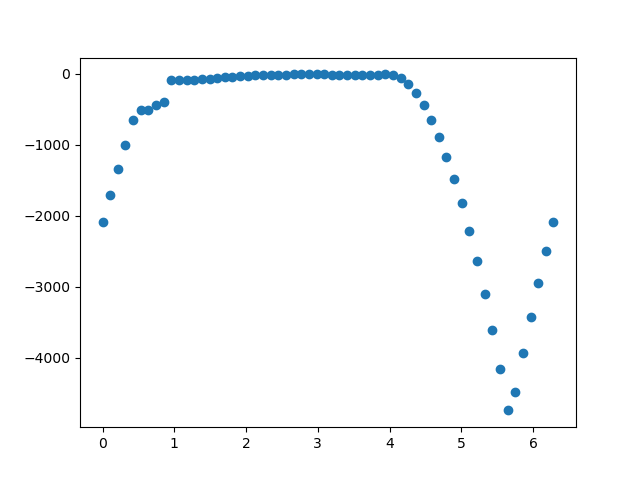
\includegraphics[width=0.7\textwidth]{pend-rand}
	\caption{(7/6/21) Zero-shot reward for PPO with known goal and a random curriculum. We note that $\pi$ is the easiest task, and $0$/$2\pi$ is the hardest, not including a few outliers.}
\end{figure}

\begin{hypothesis} (3.6.21)
	A schedule is relevant to task performance.
\end{hypothesis}
This seems to hold in practice - a constant schedule of the easiest task performs poorly, a constant schedule of a medium difficulty ($\frac{\pi}{2}$) converges faster (for PPO) but to a lower quality solution, and a constant hard schedule performs best (for PPO). A random schedule performed worse than both a hard schedule and a medium one.
Mixed schedules perform somewhere in the middle to no surprise.
We note that the worse performance of a medium schedule may be due to the pendulum environment: the ``hard'' task is symmetrical to both directions, whereas the medium schedule is not. 

\begin{figure}[h]
	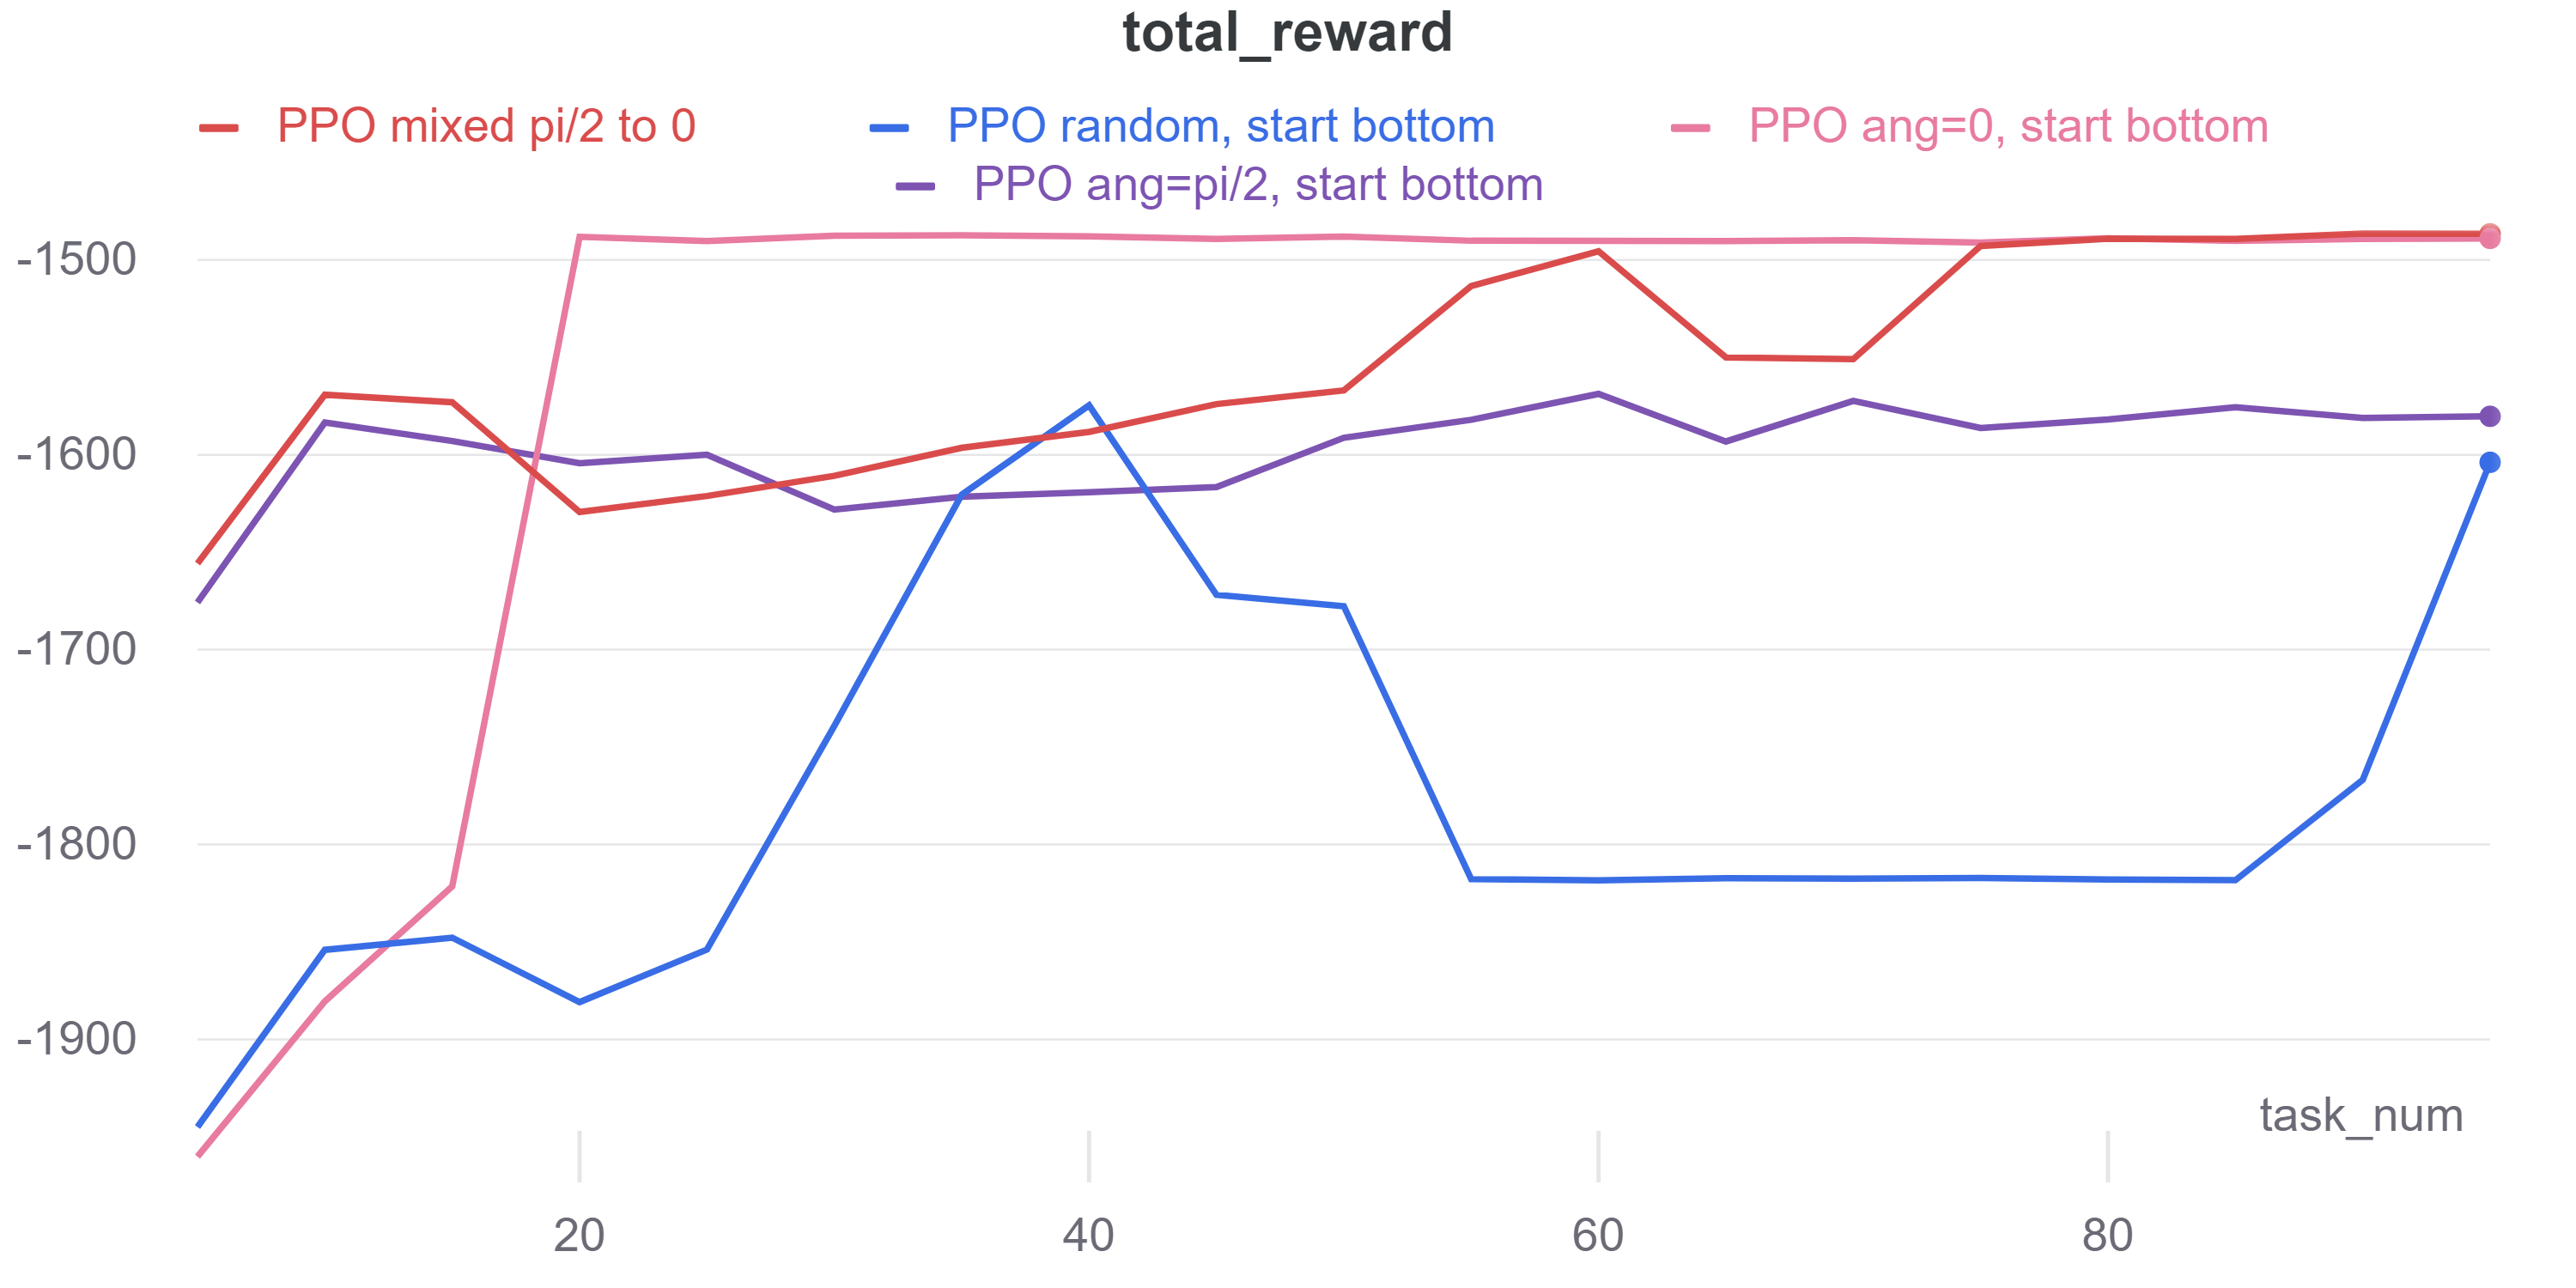
\includegraphics[width=0.7\textwidth]{pend-sched}
	\caption{(7/6/21) Zero-shot reward for PPO with several curricula.}
\end{figure}

\begin{hypothesis} (7.6.21)
	A gradual schedule is better than a random schedule.
\end{hypothesis}
To test this, we compared several simple gradual curricula. So far, this does not seem to hold when the agent is given the goal. As we see in figure \ref{figure:mixed-sched}, This hypothesis does NOT necessarily hold. We can see that the random schedule achieves the best asymptotic performance. We also see that for this student and this environment, a gradual but fast schedule is better than a more linear one, as well as a constant one, in both asymptotic and time-to-reward.


\begin{figure}[h] \label{figure:mixed-sched}
	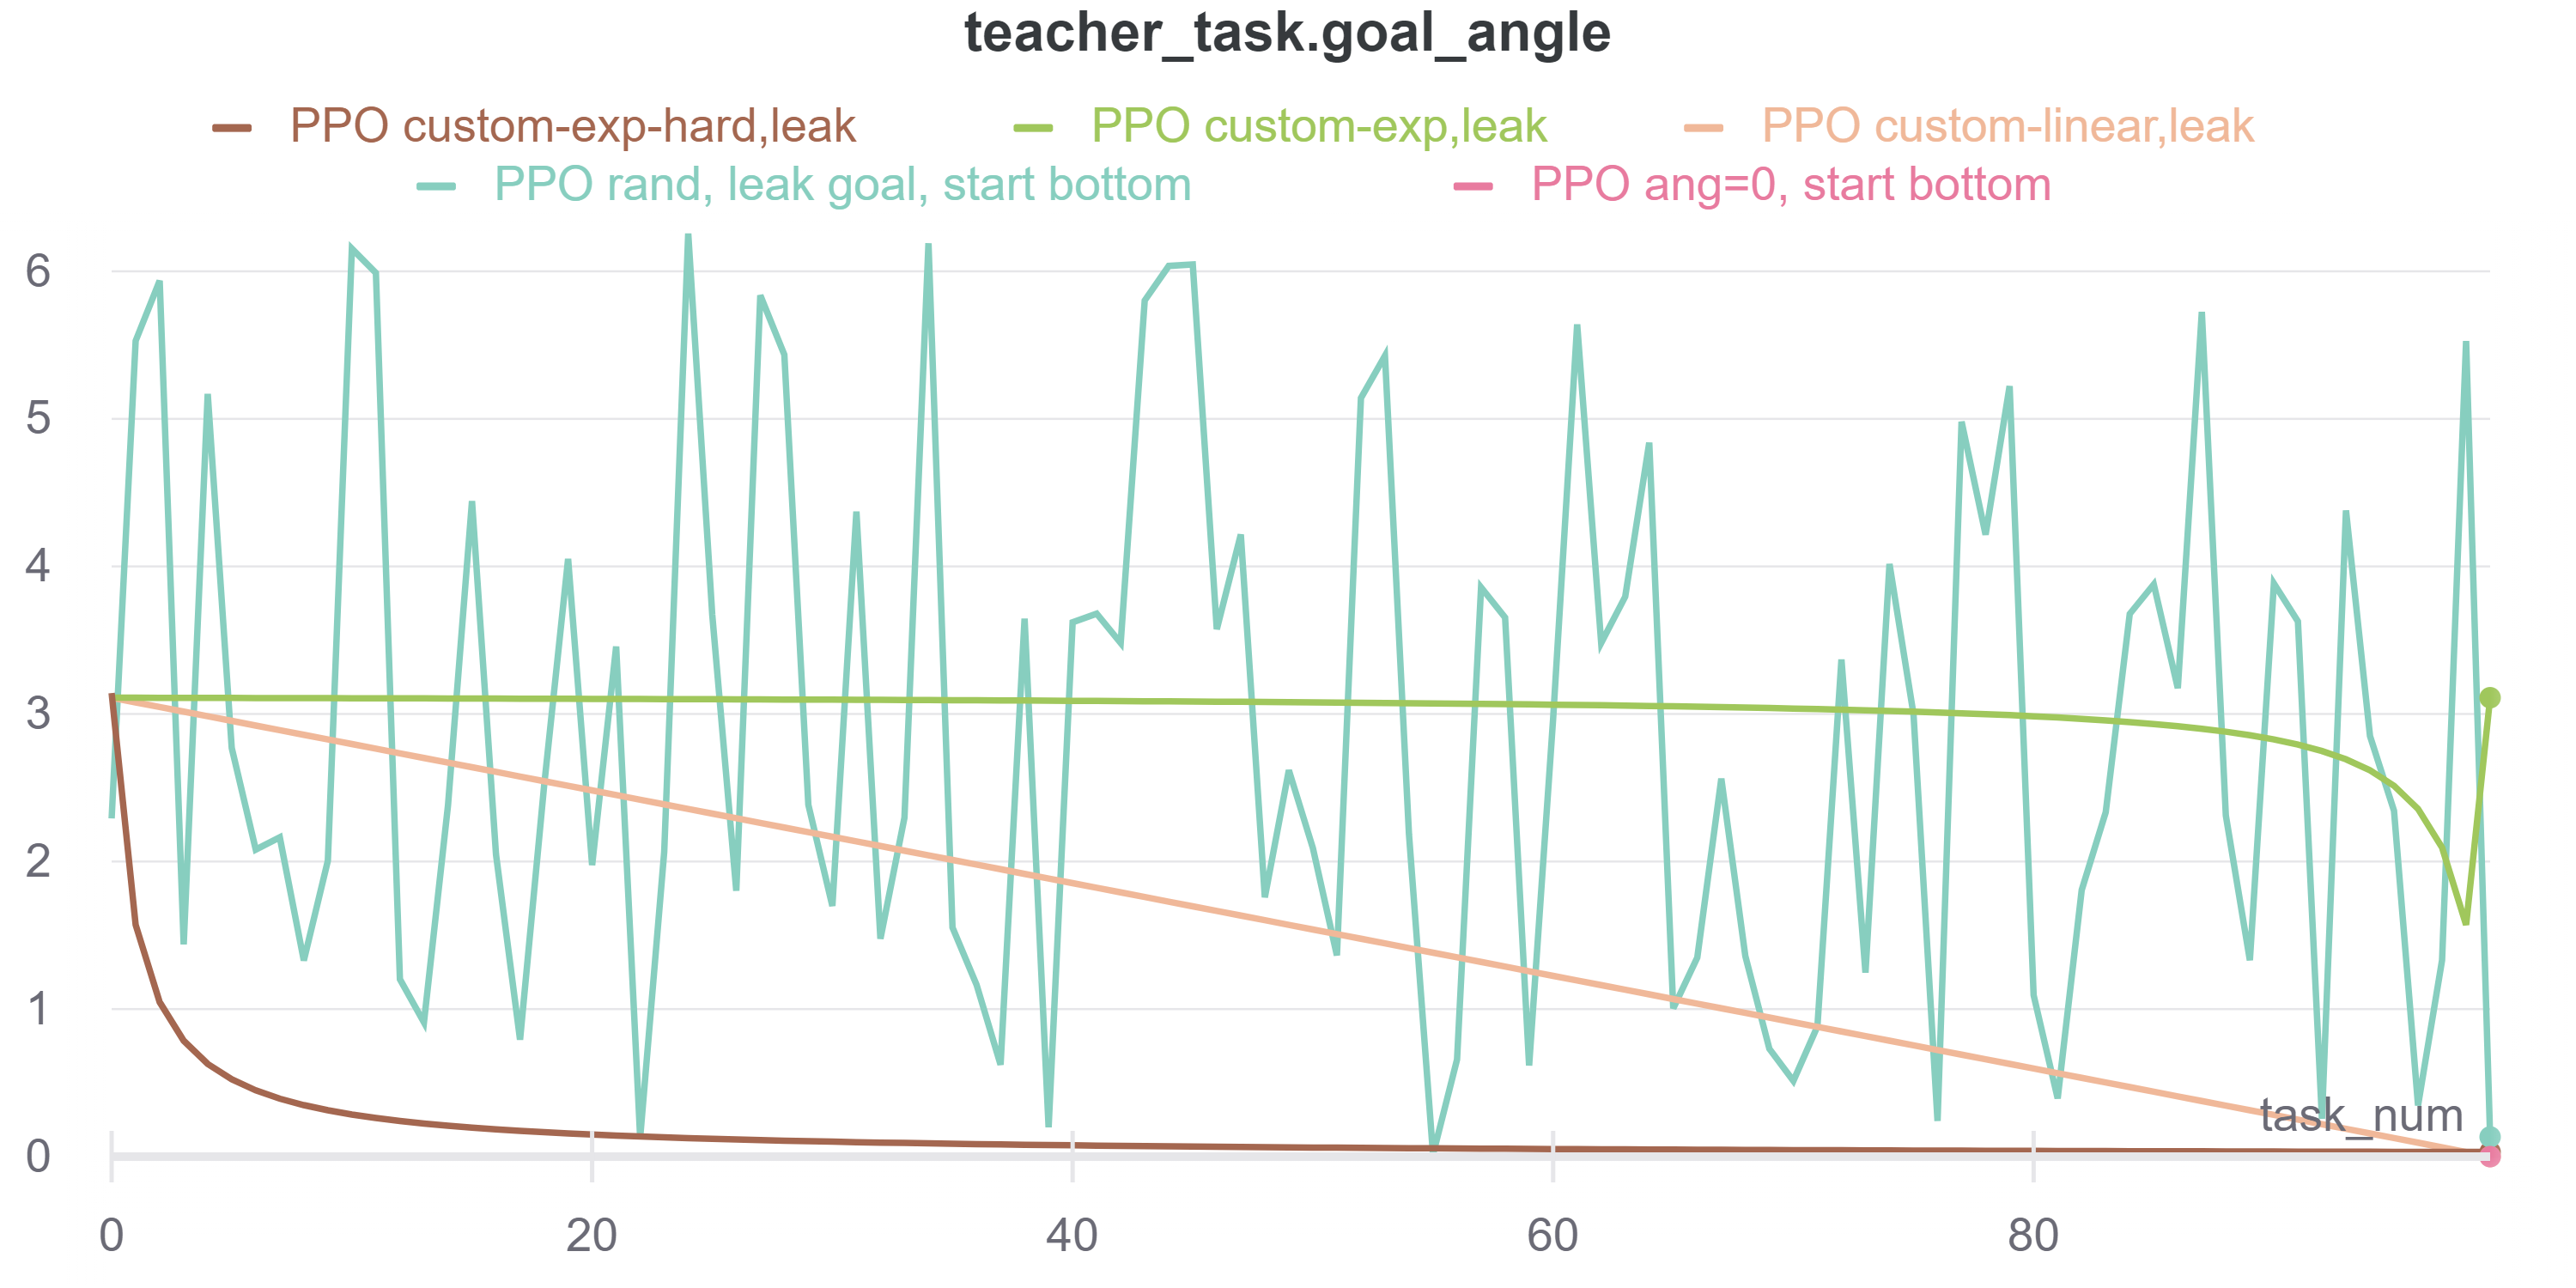
\includegraphics[width=0.5\textwidth]{mixed-sched-angles}
	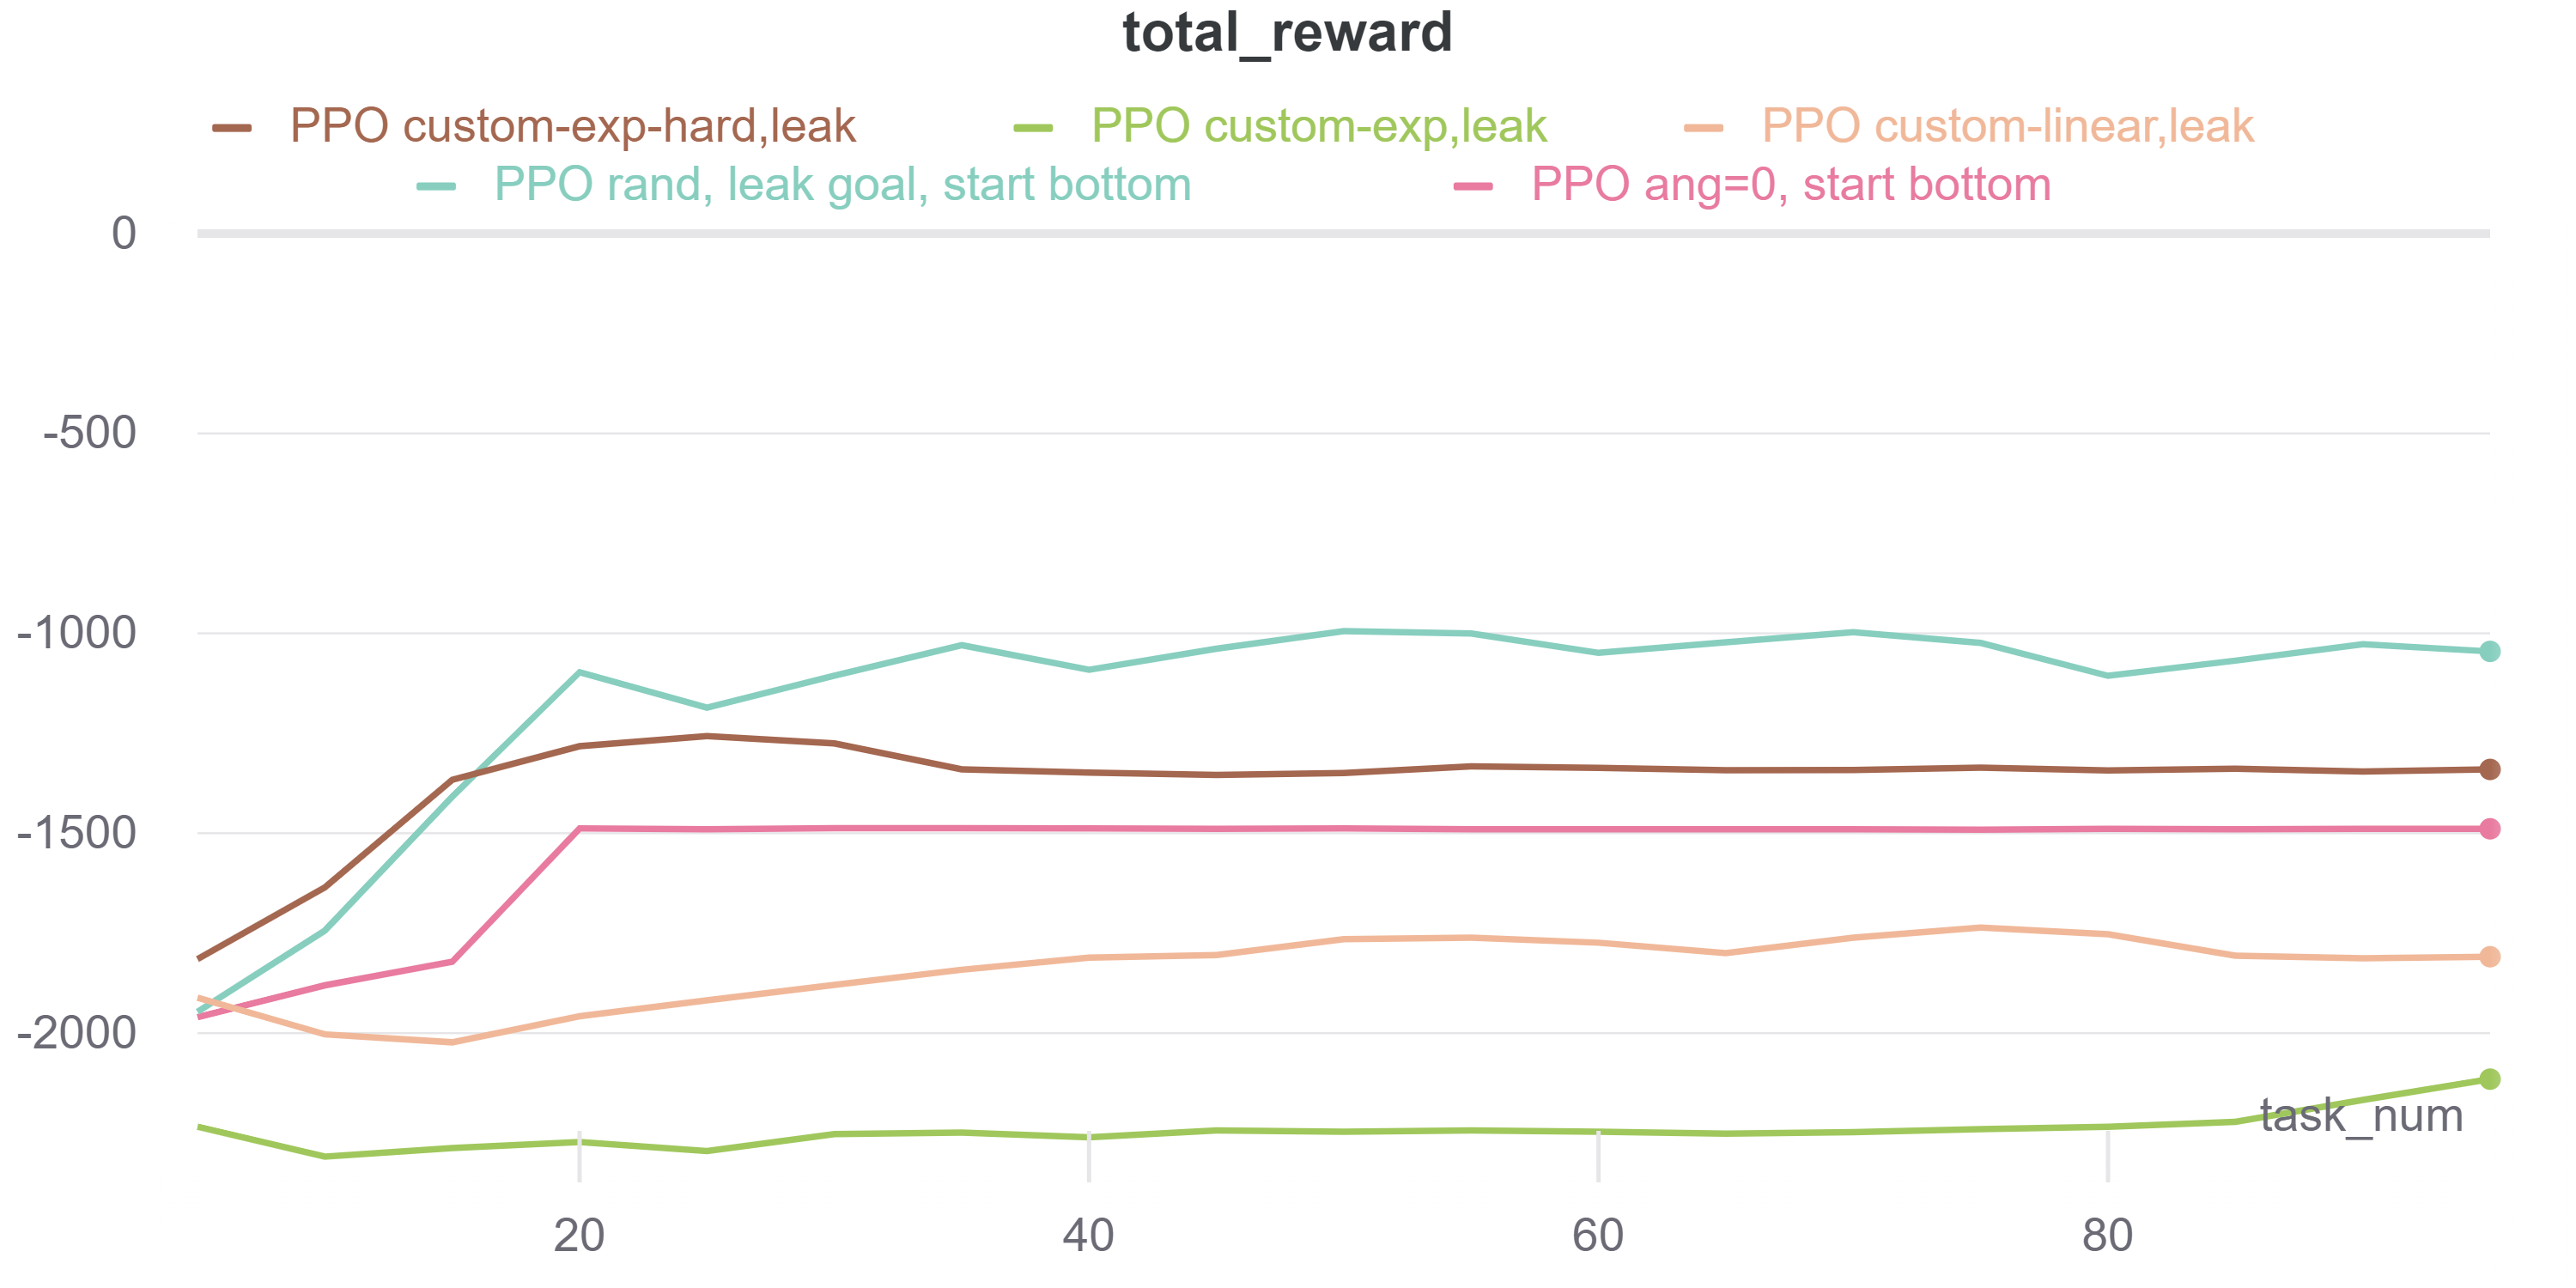
\includegraphics[width=0.5\textwidth]{mixed-sched-rewards}
	\caption{(8/6/21) Zero-shot reward for PPO, given a known goal state, with several curricula.
	The left side shows the curriculum over the training task, and the right side shows the test reward.}
\end{figure}



%%%%%%%%%%%%%%%%%%%%%%%%%%%%%%%%%%%%%%%%%%%%%%%%%%%%%%%%%%%%%%%%%%%%%%%%%%%%%%%%%%%%%%%%%%%%%%%%%
\section{*Ensemble agent ideas - 26.4.21} \label{sec:ensemble}
%%%%%%%%%%%%%%%%%%%%%%%%%%%%%%%%%%%%%%%%%%%%%%%%%%%%%%%%%%%%%%%%%%%%%%%%%%%%%%%%%%%%%%%%%%%%%%%%%

\begin{table}
	%\centering
	\caption{RL problem mapping with common solution methods. All solutions assume a dense reward function, since sparse rewards complicate all of them in similar methods.}
	\label{table-rl-problems}
	\begin{tabular}{|l | l |} 
		\hline
		\begin{tabular}{@{}c@{}}Static environment, Static dynamics \\ 
			Standard RL \\
			\end{tabular}
		 & \begin{tabular}{@{}c@{}}Static environment, Variable dynamics \\ 
		 	Meta-RL / Standard RL+Simple curricula\\
		 \end{tabular}    \\ \hline	
	 \begin{tabular}{@{}c@{}}Variable environment, Static dynamics \\ 
	 	Standard RL + curriculum  \\
	 \end{tabular}
		 & 
		 \begin{tabular}{@{}c@{}}Variable environment, Variable dynamics \\ 
		 	Unsolved \\
		 \end{tabular}  \\ \hline
	\end{tabular}
\end{table}

\begin{algorithm}[H]
	\caption{Basic curriculum-based agent}
	\label{pseudo-basic}
	\small
	\begin{algorithmic}
		\Function{Train}{$\mathcal{T}$, n, T, $\theta$}
		\State agent $\leftarrow$ \Call{Initialize}{$\theta$}
		\State teacher $\leftarrow$ \Call{Initialize}{$\theta$, $\mathcal{T}$}
		\State history $\leftarrow$ \{\}
		\For {task in n}
			\State $s_0, env$ $\leftarrow$ \Call{teacher.choose}{history, $\mathcal{T}$}
			\For {timestep in T}
				\State $a_t$ $\leftarrow$ \Call{agent.next}{$s_t$}
				\State $s_{t+1}, r_t$ $\leftarrow$ \Call{env.step}{$s_t$, $a_t$}
				\State \Call{agent.update}{$s_t$, $a_t$, $s{t+1}$, $r_t$}
			\EndFor
			\State history $\leftarrow$ history $\cup$ $\{(s_0, env, r_0, ..., r_T)\}$
		\EndFor
		\State \Return agent
		\EndFunction
	\end{algorithmic}
\end{algorithm}

Let us begin by ignoring the design of the teacher in algorithm \ref{pseudo-basic}, and assume a random curriculum for simplicity.
Looking at table \ref{table-rl-problems},  we can see that the main interesting case is a variable environment, meaning variations in start states, goals and environment elements such as obstacles.

\subsection{Action selection}

For an ensemble of model-free experts, the action selection is done with $\pi(s_t) = \sum_{i} g_i(s_t) \pi_i(s_t)$, and then actions are chosen by sampling or choosing the optimal action.

For an ensemble of model-based experts, this is done by running MPC and calculating the best action according to a (assumed known) reward model, so $a_t = argmax_a \sum_{i} g_i(s_t) \sum_{t'=0}^{H} R(M(s_{t'}, a_{t'}))$.
This can be calculated with some shooting method, using the same action sequence for each model.
It is also possible (and may be preferable for parallelization) to calculate the optimal action for each expert by itself and using $g_i$ as a weighted average by normalizing it to be a weight measure.

For both methods, we could do as previous papers did and pick only one expert (according to $g_i(s_t)$) instead.

\subsection{Agent update}

This section is fundamentally identical for model-free and model-based experts, with the only differences being how each expert uses points to update, and how experts may be unified if an adaptive number of experts is used.

The main design choice for updates is one of credit assignment - given a data point $(s_t, a_t, s_{t+1}, r_t)$, should it be applied to expert $i$ proportionally to $g_i(s_t)$ or without regarding it.
An additional minor concern is whether to apply updates immediately or aggregate in batches.

If the number of experts is not fixed, we must choose how to learn new experts and how to combine existing ones to avoid a state of adding poor new experts.
The simple approach would be to somehow choose (perhaps randomly) when to start collecting data to train a new expert. When we have gathered a large enough number of examples to train the expert, it can be evaluated alongside the others. 
In order to unify experts, it may be wise to act in a similar way to \cite{Xu2020a}, keeping a set of data points for each expert and adding the new points to an expert when unifying. This would require re-calculating $g_i(s_t)$, but that is not a high cost. 


\subsection{Choosing ensemble weights}

There is a rather large array of potential options here. It may be wise to test all of them and see what works.
These include:
\begin{itemize}
	\item A manual design, for example splitting the episode length to $k$ parts and having $g_i$ be proportional to the section in time, such that each expert has large weight in part of the episode.
	\item $g_i(s)  = entropy(s, i)$ - give high (or low) weight to experts with high action entropy in a given state. This may be a function of timestep as well.
	\item $g_i(s)  = V_i(s)$ - learn a value function for each expert (based on the return). This only really makes sense for the model-free case. 
	\item $g_i(s) = \sum_{t=0}^{h}\gamma^t V(s_t)$ - n-step version of the previous method. Relies on the reward model. Since we follow a policy for each agent, we can train a shared value function.
	\item $g_i(s) = \frac{P(s|i,s')}{\sum_j P(s|j, s')}$ - A simple likelihood estimate. Requires saving the last state and a bootstrap solution for $s_0$. We can also go farther back in time, but that seems superfluous.
	\item Learn $g_i$ with some loss function. 
	\begin{itemize}
	 	\item MSE loss (compared to $r$) with only the expert's data. This is basically the same as $g_i(s)  = V_i(s)$ but with some data selection and normalization since the expert action is different from the chosen action. Encourages convergence to a single expert.
	 	\item Some kind of discriminative loss between experts - train global $g$ as an embedding from state space to some small space (of size $k$) to maximally discriminate expert predictions, and weigh based on the most appropriate experts for a given state. It's not really clear how to achieve this. Using the predictions of other experts may be useful as a confidence measure here. Encourages very different experts.
	 	\item Some tradeoff of the above two - minimize MSE loss but penalize low KL divergence between experts, as a simple example.
	\end{itemize}
\end{itemize}

%%%%%%%%%%%%%%%%%%%%%%%%%%%%%%%%%%%%%%%%%%%%%%%%%%%%%%%%%%%%%%%%%%%%%%%%%%%%%%%%%%%%%%%%%%%%%%%%%
\clearpage
\bibliographystyle{plainnat}
\bibliography{library}

\end{document}